%%%%%%%%%%%%%%%%%%%%%%%%%%%%%%%%%%%%%%%%%%%%%%%%%%%%%%%%%%
% # Appendix: Self-Paced Reading Task Results
%%%%%%%%%%%%%%%%%%%%%%%%%%%%%%%%%%%%%%%%%%%%%%%%%%%%%%%%%%

\chapter{Self-Paced Reading Task Results}\label{app-results-spr}

%========================================================%
\section{Raw region-of-interest RTs}\label{app-spr-rt}
%========================================================%

% ORC Region 1 Means
% \DTLloaddb{dt-spr-rt}{../analysis/tables/spr_rt.csv}
% \ExplSyntaxOn
% \tl_clear:N \tblrbody
% \tl_build_begin:N \tblrbody
% \DTLforeach[\equal{\study}{ORC} \AND \equal{\region}{1}]{dt-spr-rt}{\study=study,\region=Region,\coli=Group,\colii=Environment,\coliii=Dependency,\coliv=Mean,\colv=$CI$}{\tl_build_put_right:Ne \tblrbody {\exp_not:V \coli & \exp_not:V \colii & \exp_not:V \coliii & \exp_not:V \coliv & \exp_not:V \colv\\}}
% \tl_build_end:N \tblrbody
% \ExplSyntaxOff
% \begin{longtblr}[caption={Mean raw region-of-interest RTs at Region 1 in the ORC self-paced reading task}, label={tblr:app-orc-spr-rt-r1}, expand=\tblrbody]{colspec={XXXX[r]X[r]}}\toprule
% Group & Environment & Dependency & Mean & 95\% \textit{CI}\\\midrule
% \tblrbody\bottomrule
% \end{longtblr}
% \vspace{-12pt}

% ORC Region 2 Means
% \ExplSyntaxOn
% \tl_clear:N \tblrbody
% \tl_build_begin:N \tblrbody
% \DTLforeach[\equal{\study}{ORC} \AND \equal{\region}{2}]{dt-spr-rt}{\study=study,\region=Region,\coli=Group,\colii=Environment,\coliii=Dependency,\coliv=Mean,\colv=$CI$}{\tl_build_put_right:Ne \tblrbody {\exp_not:V \coli & \exp_not:V \colii & \exp_not:V \coliii & \exp_not:V \coliv & \exp_not:V \colv\\}}
% \tl_build_end:N \tblrbody
% \ExplSyntaxOff
% \begin{longtblr}[caption={Mean raw region-of-interest RTs at Region 2 in the ORC self-paced reading task}, label={tblr:app-orc-spr-rt-r2}, expand=\tblrbody]{colspec={XXXX[r]X[r]}}\toprule
% Group & Environment & Dependency & Mean & 95\% \textit{CI}\\\midrule
% \tblrbody\bottomrule
% \end{longtblr}
% \vspace{-12pt}

% ORC Region 3 Means
% \ExplSyntaxOn
% \tl_clear:N \tblrbody
% \tl_build_begin:N \tblrbody
% \DTLforeach[\equal{\study}{ORC} \AND \equal{\region}{3}]{dt-spr-rt}{\study=study,\region=Region,\coli=Group,\colii=Environment,\coliii=Dependency,\coliv=Mean,\colv=$CI$}{\tl_build_put_right:Ne \tblrbody {\exp_not:V \coli & \exp_not:V \colii & \exp_not:V \coliii & \exp_not:V \coliv & \exp_not:V \colv\\}}
% \tl_build_end:N \tblrbody
% \ExplSyntaxOff
% \begin{longtblr}[caption={Mean raw region-of-interest RTs at Region 3 in the ORC self-paced reading task}, label={tblr:app-orc-spr-rt-r3}, expand=\tblrbody]{colspec={XXXX[r]X[r]}}\toprule
% Group & Environment & Dependency & Mean & 95\% \textit{CI}\\\midrule
% \tblrbody\bottomrule
% \end{longtblr}
% \vspace{-12pt}

% SRC Region 1 Means
% \ExplSyntaxOn
% \tl_clear:N \tblrbody
% \tl_build_begin:N \tblrbody
% \DTLforeach[\equal{\study}{SRC} \AND \equal{\region}{1}]{dt-spr-rt}{\study=study,\region=Region,\coli=Group,\colii=Environment,\coliii=Dependency,\coliv=Mean,\colv=$CI$}{\tl_build_put_right:Ne \tblrbody {\exp_not:V \coli & \exp_not:V \colii & \exp_not:V \coliii & \exp_not:V \coliv & \exp_not:V \colv\\}}
% \tl_build_end:N \tblrbody
% \ExplSyntaxOff
% \begin{longtblr}[caption={Mean raw region-of-interest RTs at Region 1 in the SRC self-paced reading task}, label={tblr:app-src-spr-rt-r1}, expand=\tblrbody]{colspec={XXXX[r]X[r]}}\toprule
% Group & Environment & Dependency & Mean & 95\% \textit{CI}\\\midrule
% \tblrbody\bottomrule
% \end{longtblr}
% \vspace{-12pt}

% SRC Region 2 Means
% \ExplSyntaxOn
% \tl_clear:N \tblrbody
% \tl_build_begin:N \tblrbody
% \DTLforeach[\equal{\study}{SRC} \AND \equal{\region}{2}]{dt-spr-rt}{\study=study,\region=Region,\coli=Group,\colii=Environment,\coliii=Dependency,\coliv=Mean,\colv=$CI$}{\tl_build_put_right:Ne \tblrbody {\exp_not:V \coli & \exp_not:V \colii & \exp_not:V \coliii & \exp_not:V \coliv & \exp_not:V \colv\\}}
% \tl_build_end:N \tblrbody
% \ExplSyntaxOff
% \begin{longtblr}[caption={Mean raw region-of-interest RTs at Region 2 in the SRC self-paced reading task}, label={tblr:app-src-spr-rt-r2}, expand=\tblrbody]{colspec={XXXX[r]X[r]}}\toprule
% Group & Environment & Dependency & Mean & 95\% \textit{CI}\\\midrule
% \tblrbody\bottomrule
% \end{longtblr}
% \vspace{-12pt}

% SRC Region 3 Means
% \ExplSyntaxOn
% \tl_clear:N \tblrbody
% \tl_build_begin:N \tblrbody
% \DTLforeach[\equal{\study}{SRC} \AND \equal{\region}{3}]{dt-spr-rt}{\study=study,\region=Region,\coli=Group,\colii=Environment,\coliii=Dependency,\coliv=Mean,\colv=$CI$}{\tl_build_put_right:Ne \tblrbody {\exp_not:V \coli & \exp_not:V \colii & \exp_not:V \coliii & \exp_not:V \coliv & \exp_not:V \colv\\}}
% \tl_build_end:N \tblrbody
% \ExplSyntaxOff
% \begin{longtblr}[caption={Mean raw region-of-interest RTs at Region 3 in the SRC self-paced reading task}, label={tblr:app-src-spr-rt-r3}, expand=\tblrbody]{colspec={XXXX[r]X[r]}}\toprule
% Group & Environment & Dependency & Mean & 95\% \textit{CI}\\\midrule
% \tblrbody\bottomrule
% \end{longtblr}
% \vspace{-12pt}

% ORC Figure
\begin{figure}
\caption{Mean raw region-of-interest RTs in the ORC self-paced reading task} \label{fig:app-orc-spr-rt}
\raggedright\setstretch{1}
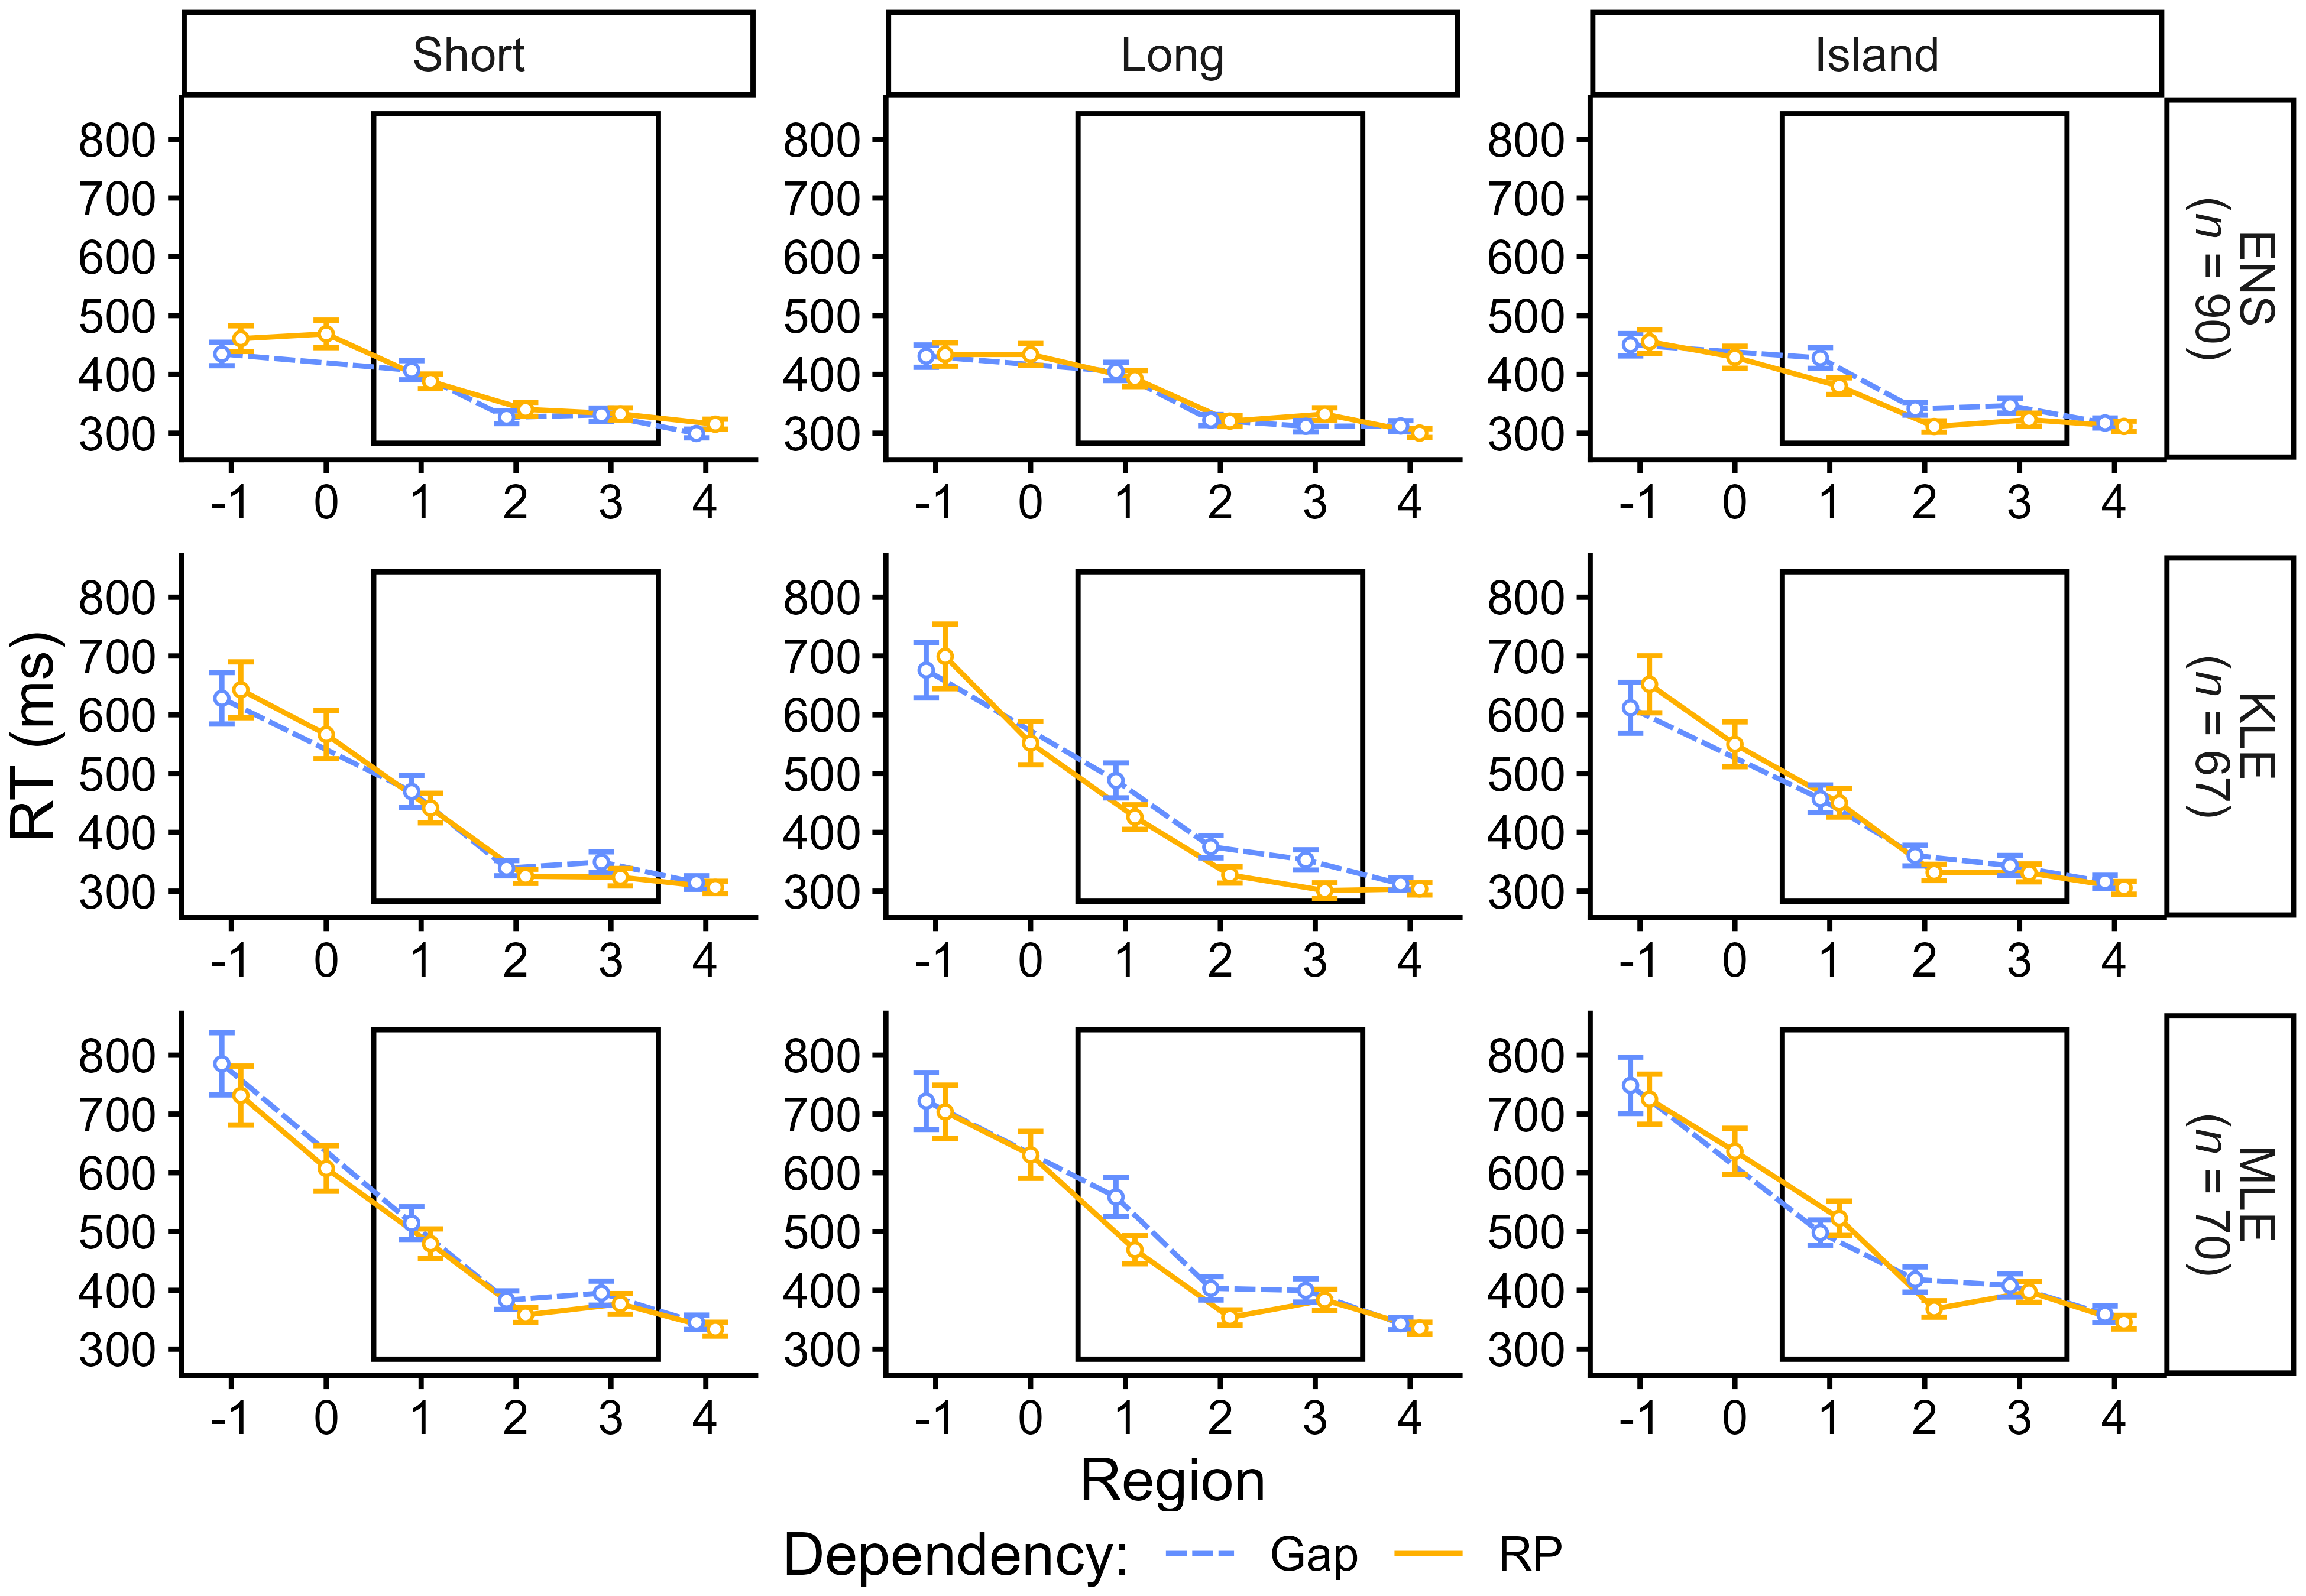
\includegraphics{../analysis/plots/orc_spr_rt.png}
\textit{Note}. Region 0 is the gap/RP; error bars are 95\% $CI$s; rectangle indicates regions of interest.
\vspace{-12pt}
\end{figure}

% SRC Figure
\begin{figure}
\caption{Mean raw region-of-interest RTs in the SRC self-paced reading task} \label{fig:app-src-spr-rt}
\raggedright\setstretch{1}
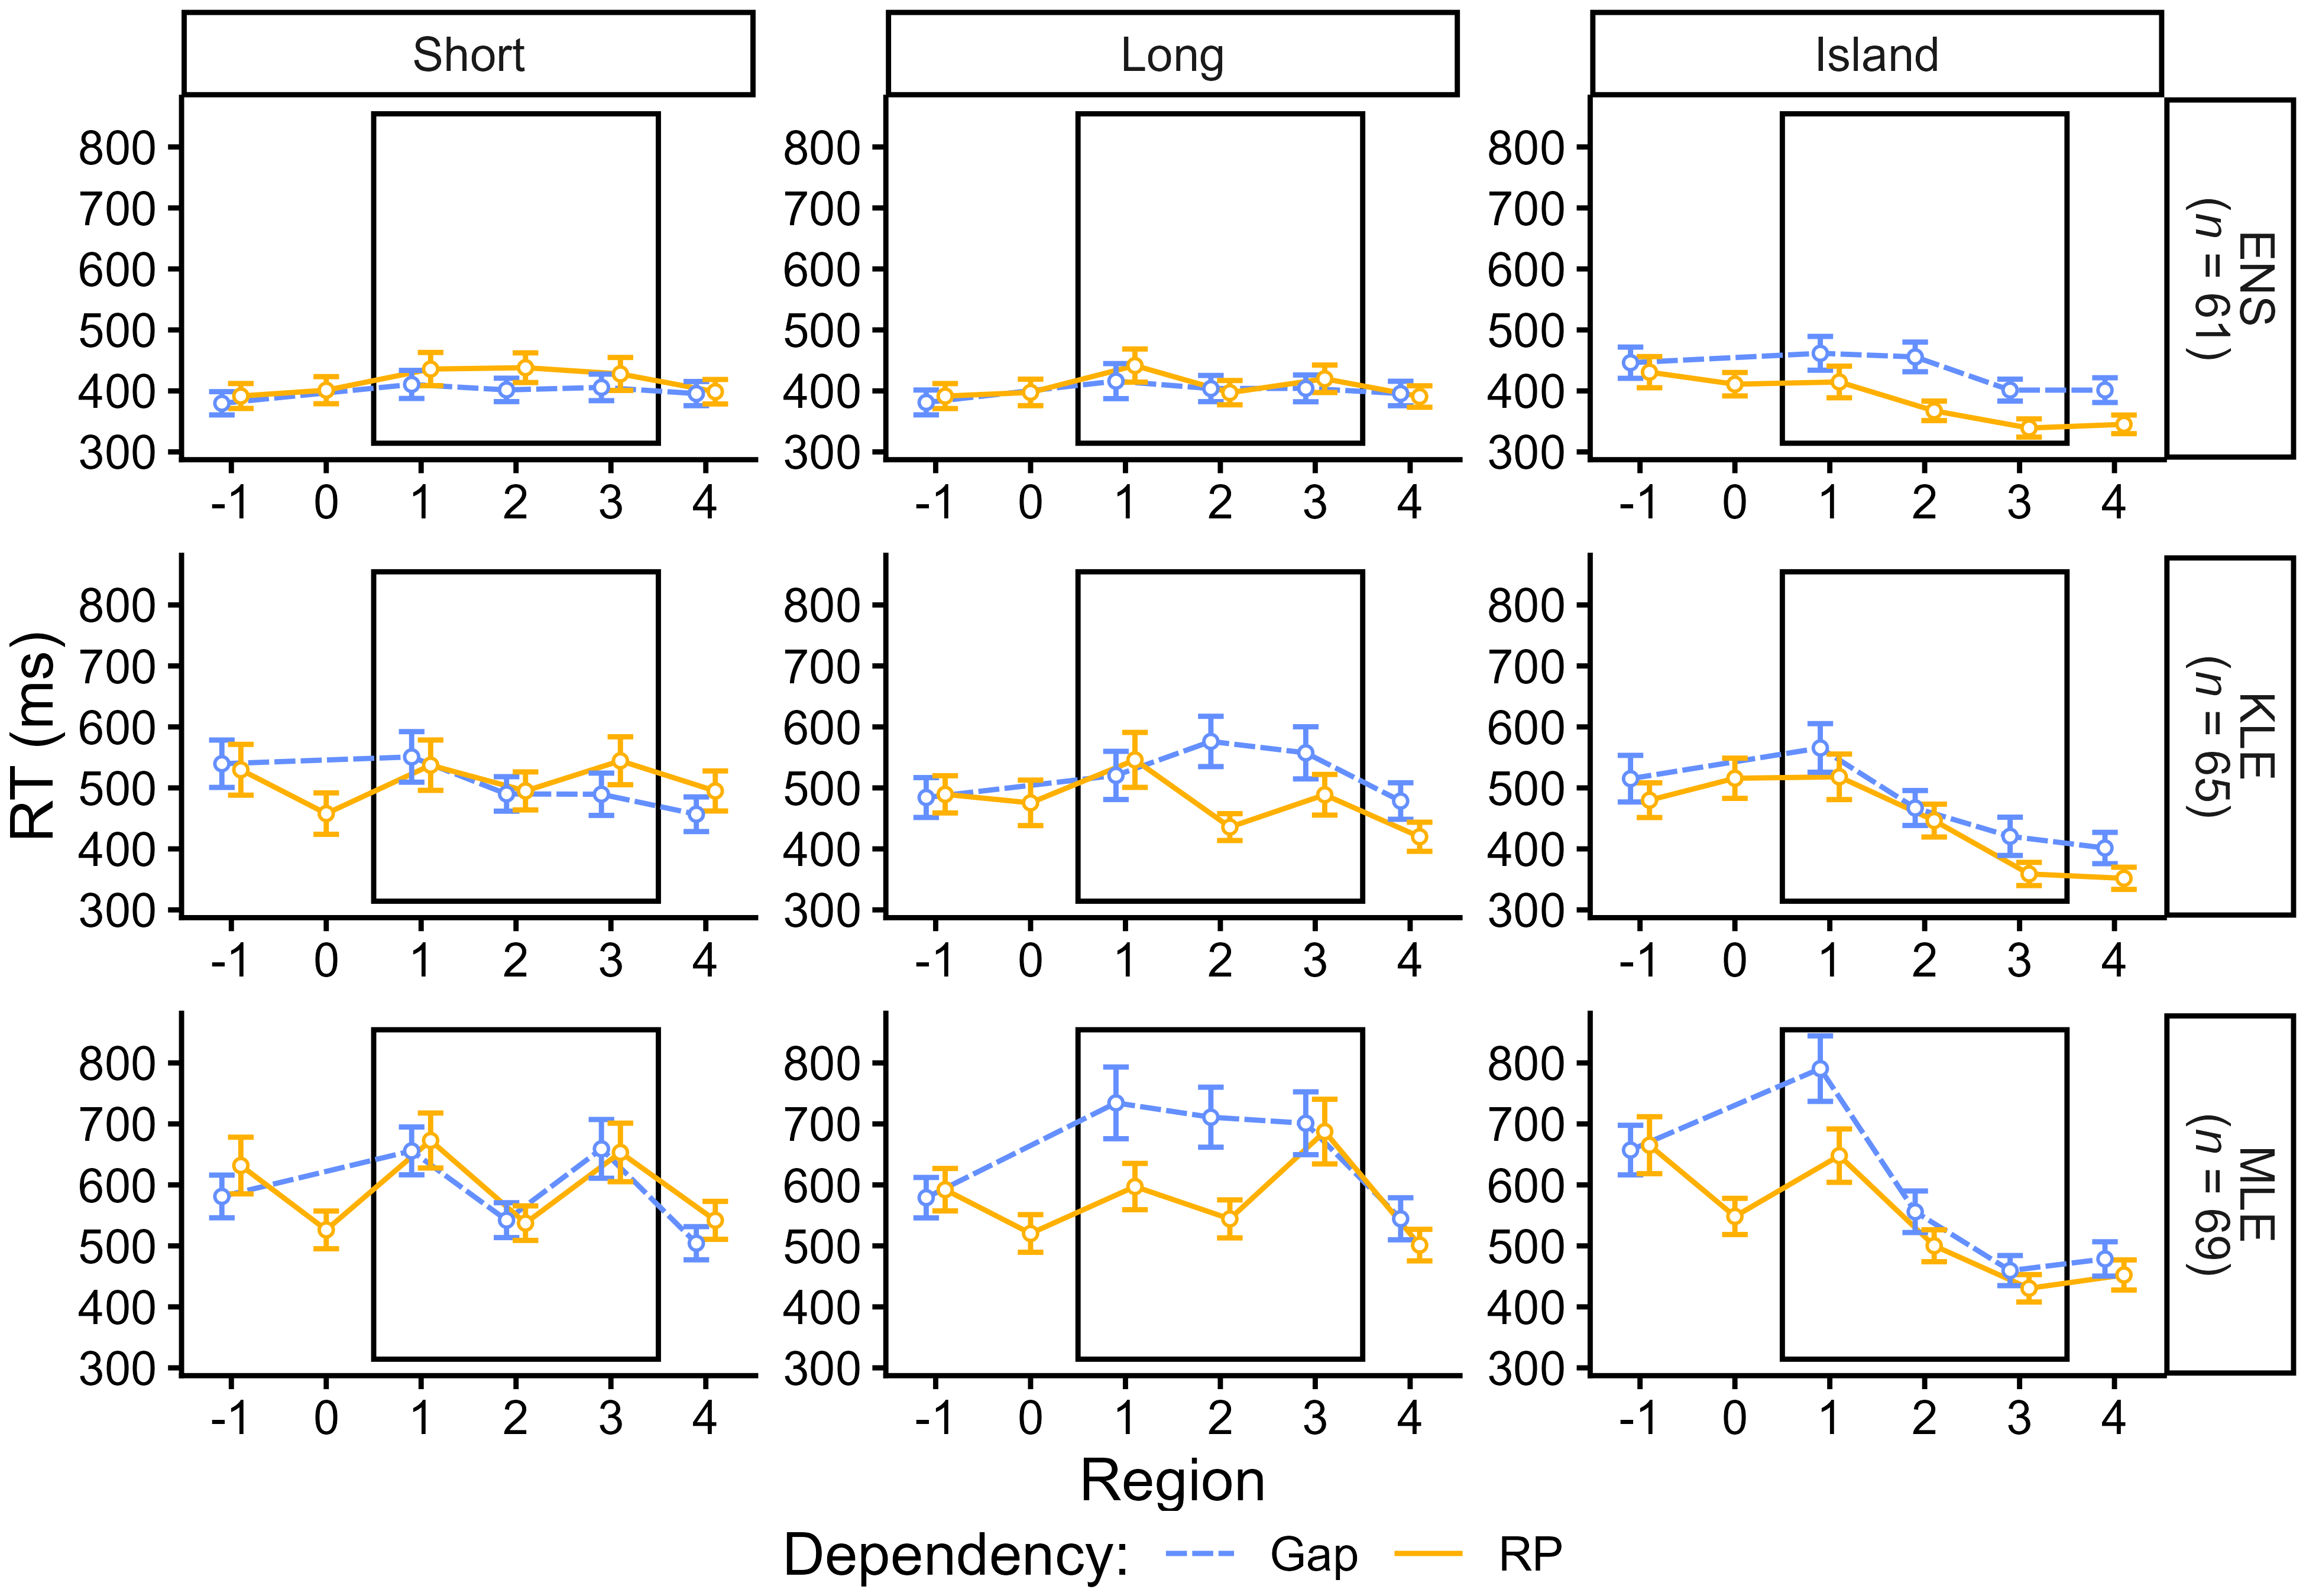
\includegraphics{../analysis/plots/src_spr_rt.png}
\textit{Note}. Region 0 is the gap/RP; error bars are 95\% $CI$s; rectangle indicates regions of interest.
\end{figure}

%========================================================%
\section{Log-transformed region-of-interest RTs}\label{app-spr-logrt}
%========================================================%

% ORC Region 1 Means
% \DTLloaddb{dt-spr-logrt}{../analysis/tables/spr_logrt.csv}
% \ExplSyntaxOn
% \tl_clear:N \tblrbody
% \tl_build_begin:N \tblrbody
% \DTLforeach[\equal{\study}{ORC} \AND \equal{\region}{1}]{dt-spr-logrt}{\study=study,\region=Region,\coli=Group,\colii=Environment,\coliii=Dependency,\coliv=Mean,\colv=$CI$}{\tl_build_put_right:Ne \tblrbody {\exp_not:V \coli & \exp_not:V \colii & \exp_not:V \coliii & \exp_not:V \coliv & \exp_not:V \colv\\}}
% \tl_build_end:N \tblrbody
% \ExplSyntaxOff
% \begin{longtblr}[caption={Mean region-of-interest log RTs at Region 1 in the ORC self-paced reading task}, label={tblr:app-orc-spr-logrt-r1}, expand=\tblrbody]{colspec={XXXX[r]X[r]}}\toprule
% Group & Environment & Dependency & Mean & 95\% \textit{CI}\\\midrule
% \tblrbody\bottomrule
% \end{longtblr}
% \vspace{-12pt}

% ORC Region 2 Means 
% \ExplSyntaxOn
% \tl_clear:N \tblrbody
% \tl_build_begin:N \tblrbody
% \DTLforeach[\equal{\study}{ORC} \AND \equal{\region}{2}]{dt-spr-logrt}{\study=study,\region=Region,\coli=Group,\colii=Environment,\coliii=Dependency,\coliv=Mean,\colv=$CI$}{\tl_build_put_right:Ne \tblrbody {\exp_not:V \coli & \exp_not:V \colii & \exp_not:V \coliii & \exp_not:V \coliv & \exp_not:V \colv\\}}
% \tl_build_end:N \tblrbody
% \ExplSyntaxOff
% \begin{longtblr}[caption={Mean region-of-interest log RTs at Region 2 in the ORC self-paced reading task}, label={tblr:app-orc-spr-logrt-r2}, expand=\tblrbody]{colspec={XXXX[r]X[r]}}\toprule
% Group & Environment & Dependency & Mean & 95\% \textit{CI}\\\midrule
% \tblrbody\bottomrule
% \end{longtblr}
% \vspace{-12pt}

% ORC Region 3 Means
% \ExplSyntaxOn
% \tl_clear:N \tblrbody
% \tl_build_begin:N \tblrbody
% \DTLforeach[\equal{\study}{ORC} \AND \equal{\region}{3}]{dt-spr-logrt}{\study=study,\region=Region,\coli=Group,\colii=Environment,\coliii=Dependency,\coliv=Mean,\colv=$CI$}{\tl_build_put_right:Ne \tblrbody {\exp_not:V \coli & \exp_not:V \colii & \exp_not:V \coliii & \exp_not:V \coliv & \exp_not:V \colv\\}}
% \tl_build_end:N \tblrbody
% \ExplSyntaxOff
% \begin{longtblr}[caption={Mean region-of-interest log RTs at Region 3 in the ORC self-paced reading task}, label={tblr:app-orc-spr-logrt-r3}, expand=\tblrbody]{colspec={XXXX[r]X[r]}}\toprule
% Group & Environment & Dependency & Mean & 95\% \textit{CI}\\\midrule
% \tblrbody\bottomrule
% \end{longtblr}
% \vspace{-12pt}

% SRC Region 1 Means
% \ExplSyntaxOn
% \tl_clear:N \tblrbody
% \tl_build_begin:N \tblrbody
% \DTLforeach[\equal{\study}{SRC} \AND \equal{\region}{1}]{dt-spr-logrt}{\study=study,\region=Region,\coli=Group,\colii=Environment,\coliii=Dependency,\coliv=Mean,\colv=$CI$}{\tl_build_put_right:Ne \tblrbody {\exp_not:V \coli & \exp_not:V \colii & \exp_not:V \coliii & \exp_not:V \coliv & \exp_not:V \colv\\}}
% \tl_build_end:N \tblrbody
% \ExplSyntaxOff
% \begin{longtblr}[caption={Mean region-of-interest log RTs at Region 1 in the SRC self-paced reading task}, label={tblr:app-src-spr-logrt-r1}, expand=\tblrbody]{colspec={XXXX[r]X[r]}}\toprule
% Group & Environment & Dependency & Mean & 95\% \textit{CI}\\\midrule
% \tblrbody\bottomrule
% \end{longtblr}
% \vspace{-12pt}

% SRC Region 2 Means
% \ExplSyntaxOn
% \tl_clear:N \tblrbody
% \tl_build_begin:N \tblrbody
% \DTLforeach[\equal{\study}{SRC} \AND \equal{\region}{2}]{dt-spr-logrt}{\study=study,\region=Region,\coli=Group,\colii=Environment,\coliii=Dependency,\coliv=Mean,\colv=$CI$}{\tl_build_put_right:Ne \tblrbody {\exp_not:V \coli & \exp_not:V \colii & \exp_not:V \coliii & \exp_not:V \coliv & \exp_not:V \colv\\}}
% \tl_build_end:N \tblrbody
% \ExplSyntaxOff
% \begin{longtblr}[caption={Mean region-of-interest log RTs at Region 2 in the SRC self-paced reading task}, label={tblr:app-src-spr-logrt-r2}, expand=\tblrbody]{colspec={XXXX[r]X[r]}}\toprule
% Group & Environment & Dependency & Mean & 95\% \textit{CI}\\\midrule
% \tblrbody\bottomrule
% \end{longtblr}
% \vspace{-12pt}

% SRC Region 3 Means
% \ExplSyntaxOn
% \tl_clear:N \tblrbody
% \tl_build_begin:N \tblrbody
% \DTLforeach[\equal{\study}{SRC} \AND \equal{\region}{3}]{dt-spr-logrt}{\study=study,\region=Region,\coli=Group,\colii=Environment,\coliii=Dependency,\coliv=Mean,\colv=$CI$}{\tl_build_put_right:Ne \tblrbody {\exp_not:V \coli & \exp_not:V \colii & \exp_not:V \coliii & \exp_not:V \coliv & \exp_not:V \colv\\}}
% \tl_build_end:N \tblrbody
% \ExplSyntaxOff
% \begin{longtblr}[caption={Mean region-of-interest log RTs at Region 3 in the SRC self-paced reading task}, label={tblr:app-src-spr-logrt-r3}, expand=\tblrbody]{colspec={XXXX[r]X[r]}}\toprule
% Group & Environment & Dependency & Mean & 95\% \textit{CI}\\\midrule
% \tblrbody\bottomrule
% \end{longtblr}
% \vspace{-12pt}

% ORC Figure
% \begin{figure}
% \caption[height=4in]{Mean region-of-interest log RTs in the ORC self-paced reading task} \label{fig:app-orc-spr-logrt}
% \raggedright\setstretch{1}
% 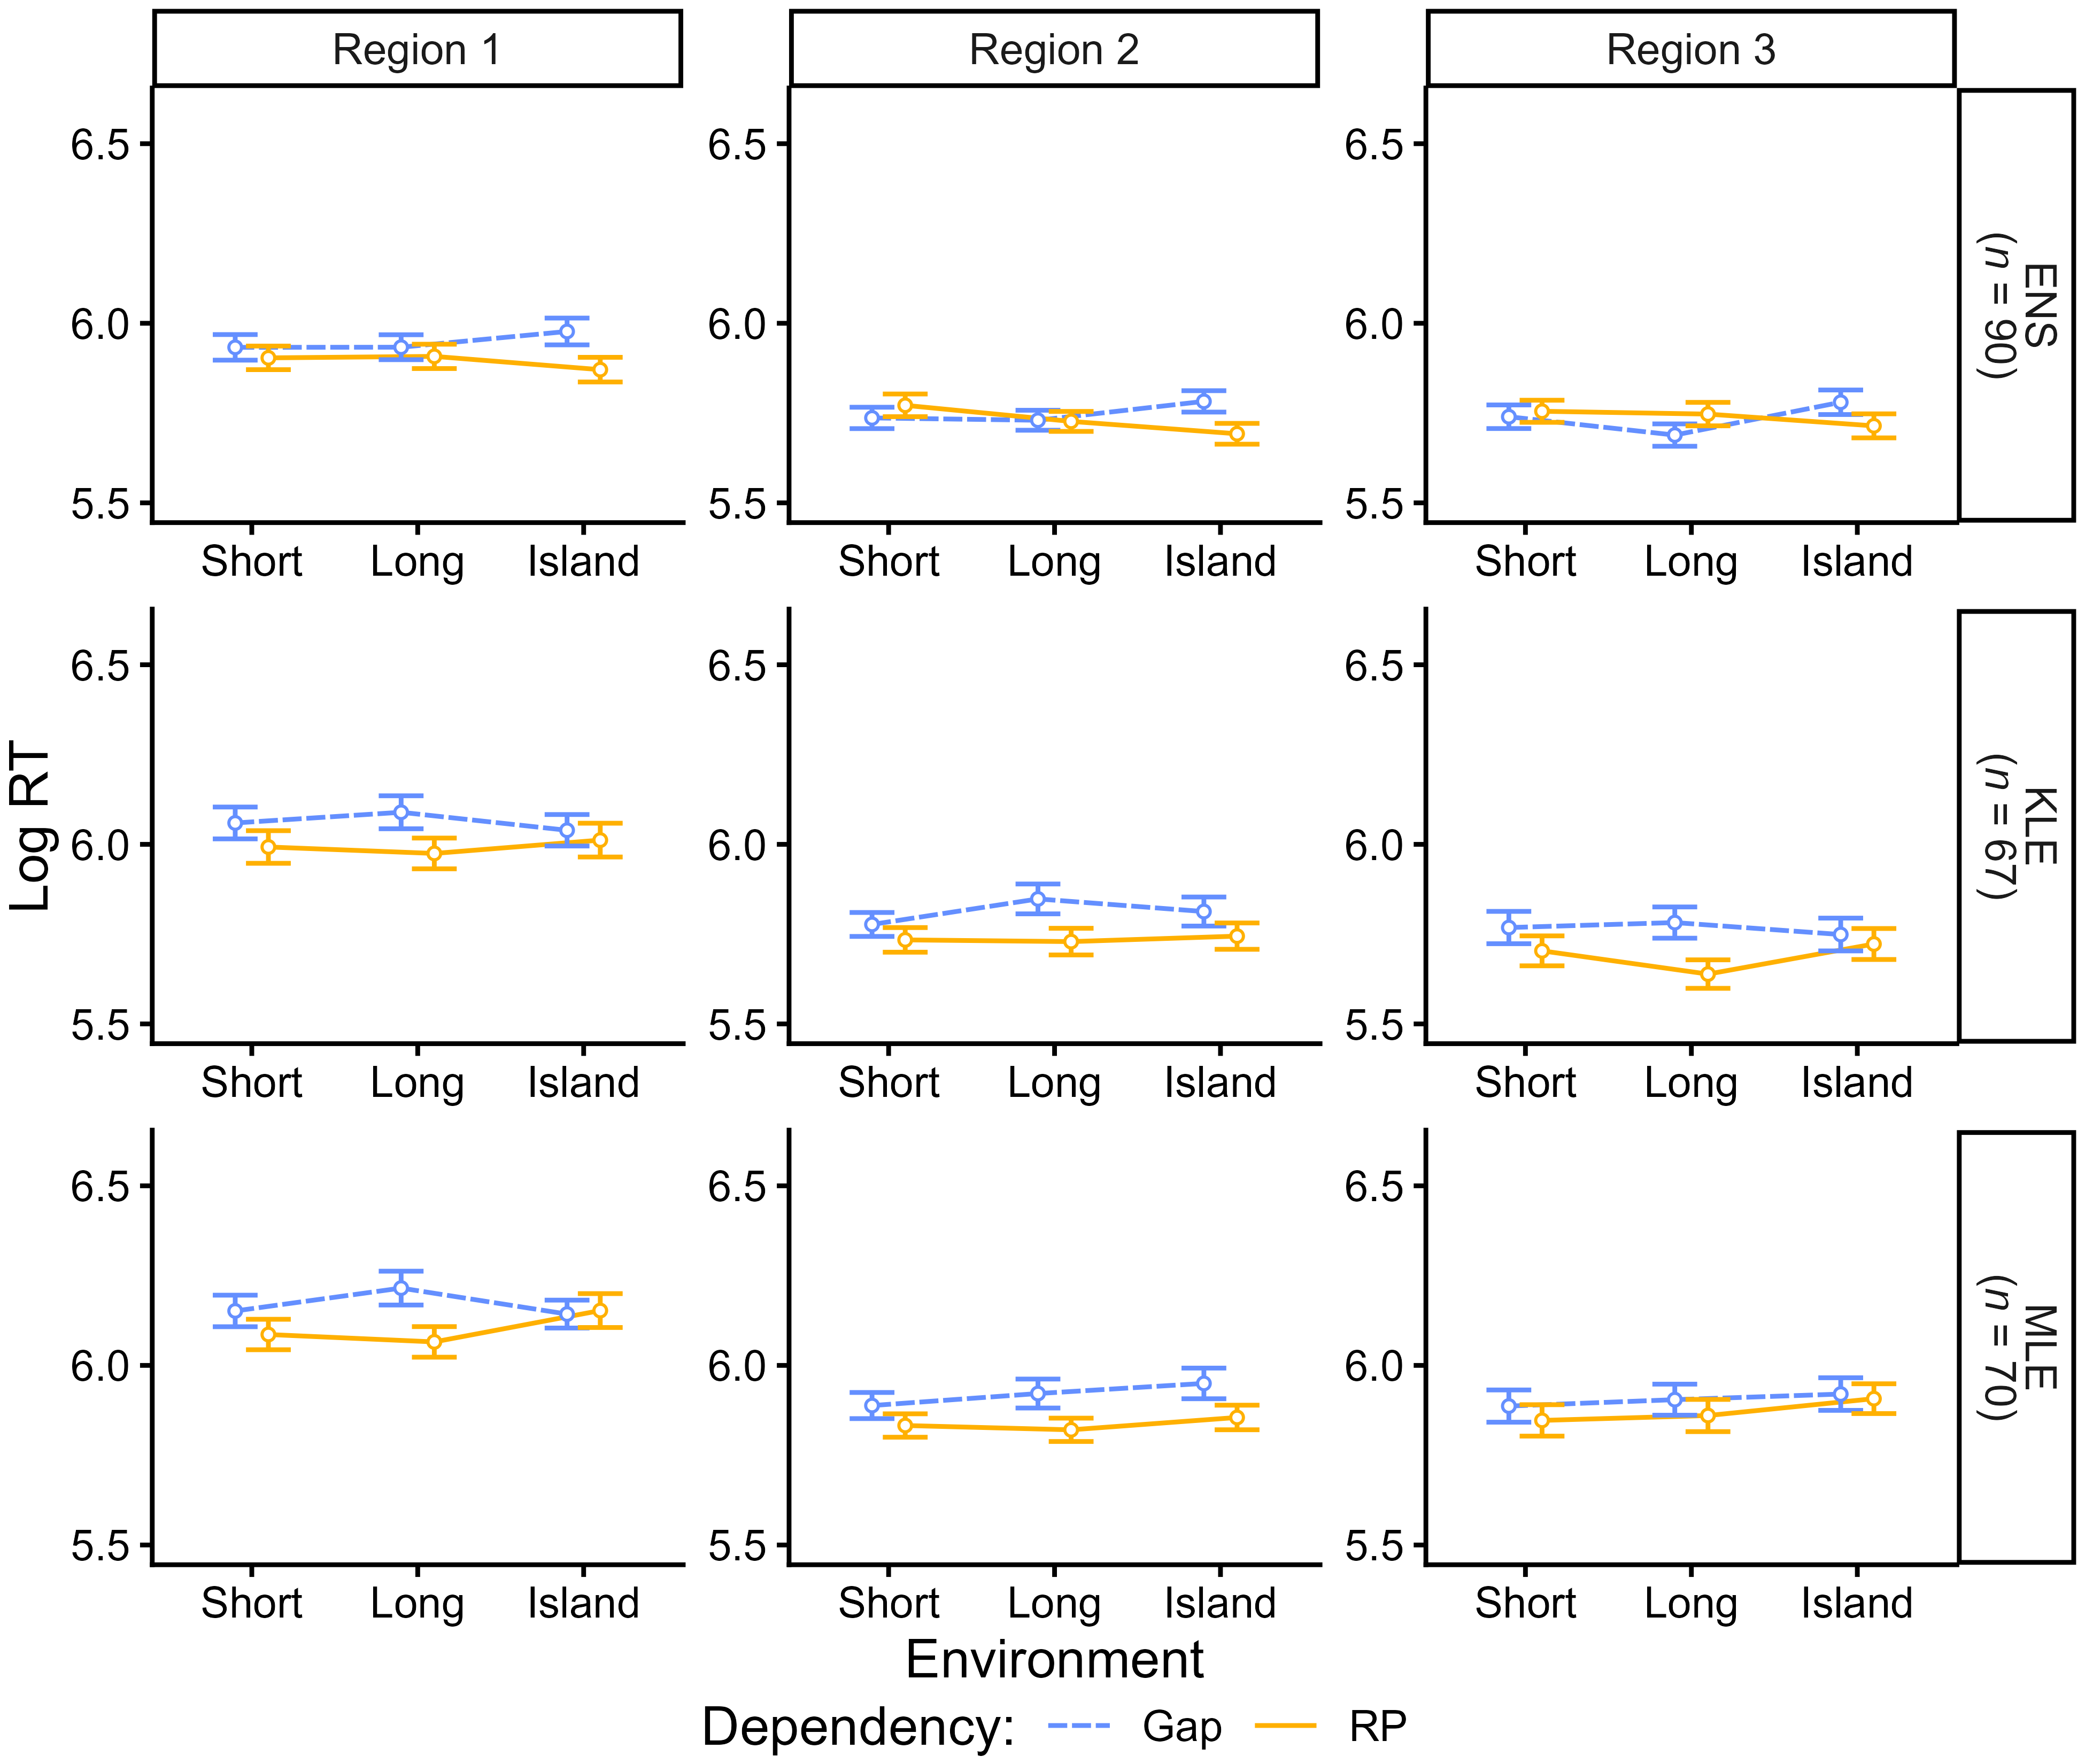
\includegraphics{../analysis/plots/orc_spr_logrt2.png}
% \textit{Note}. Error bars are 95\% $CI$s.
% \vspace{-12pt}
% \end{figure}

% SRC Figure
% \begin{figure}
% \caption[height=4in]{Mean region-of-interest log RTs in the SRC self-paced reading task} \label{fig:app-src-spr-logrt}
% \raggedright\setstretch{1}
% 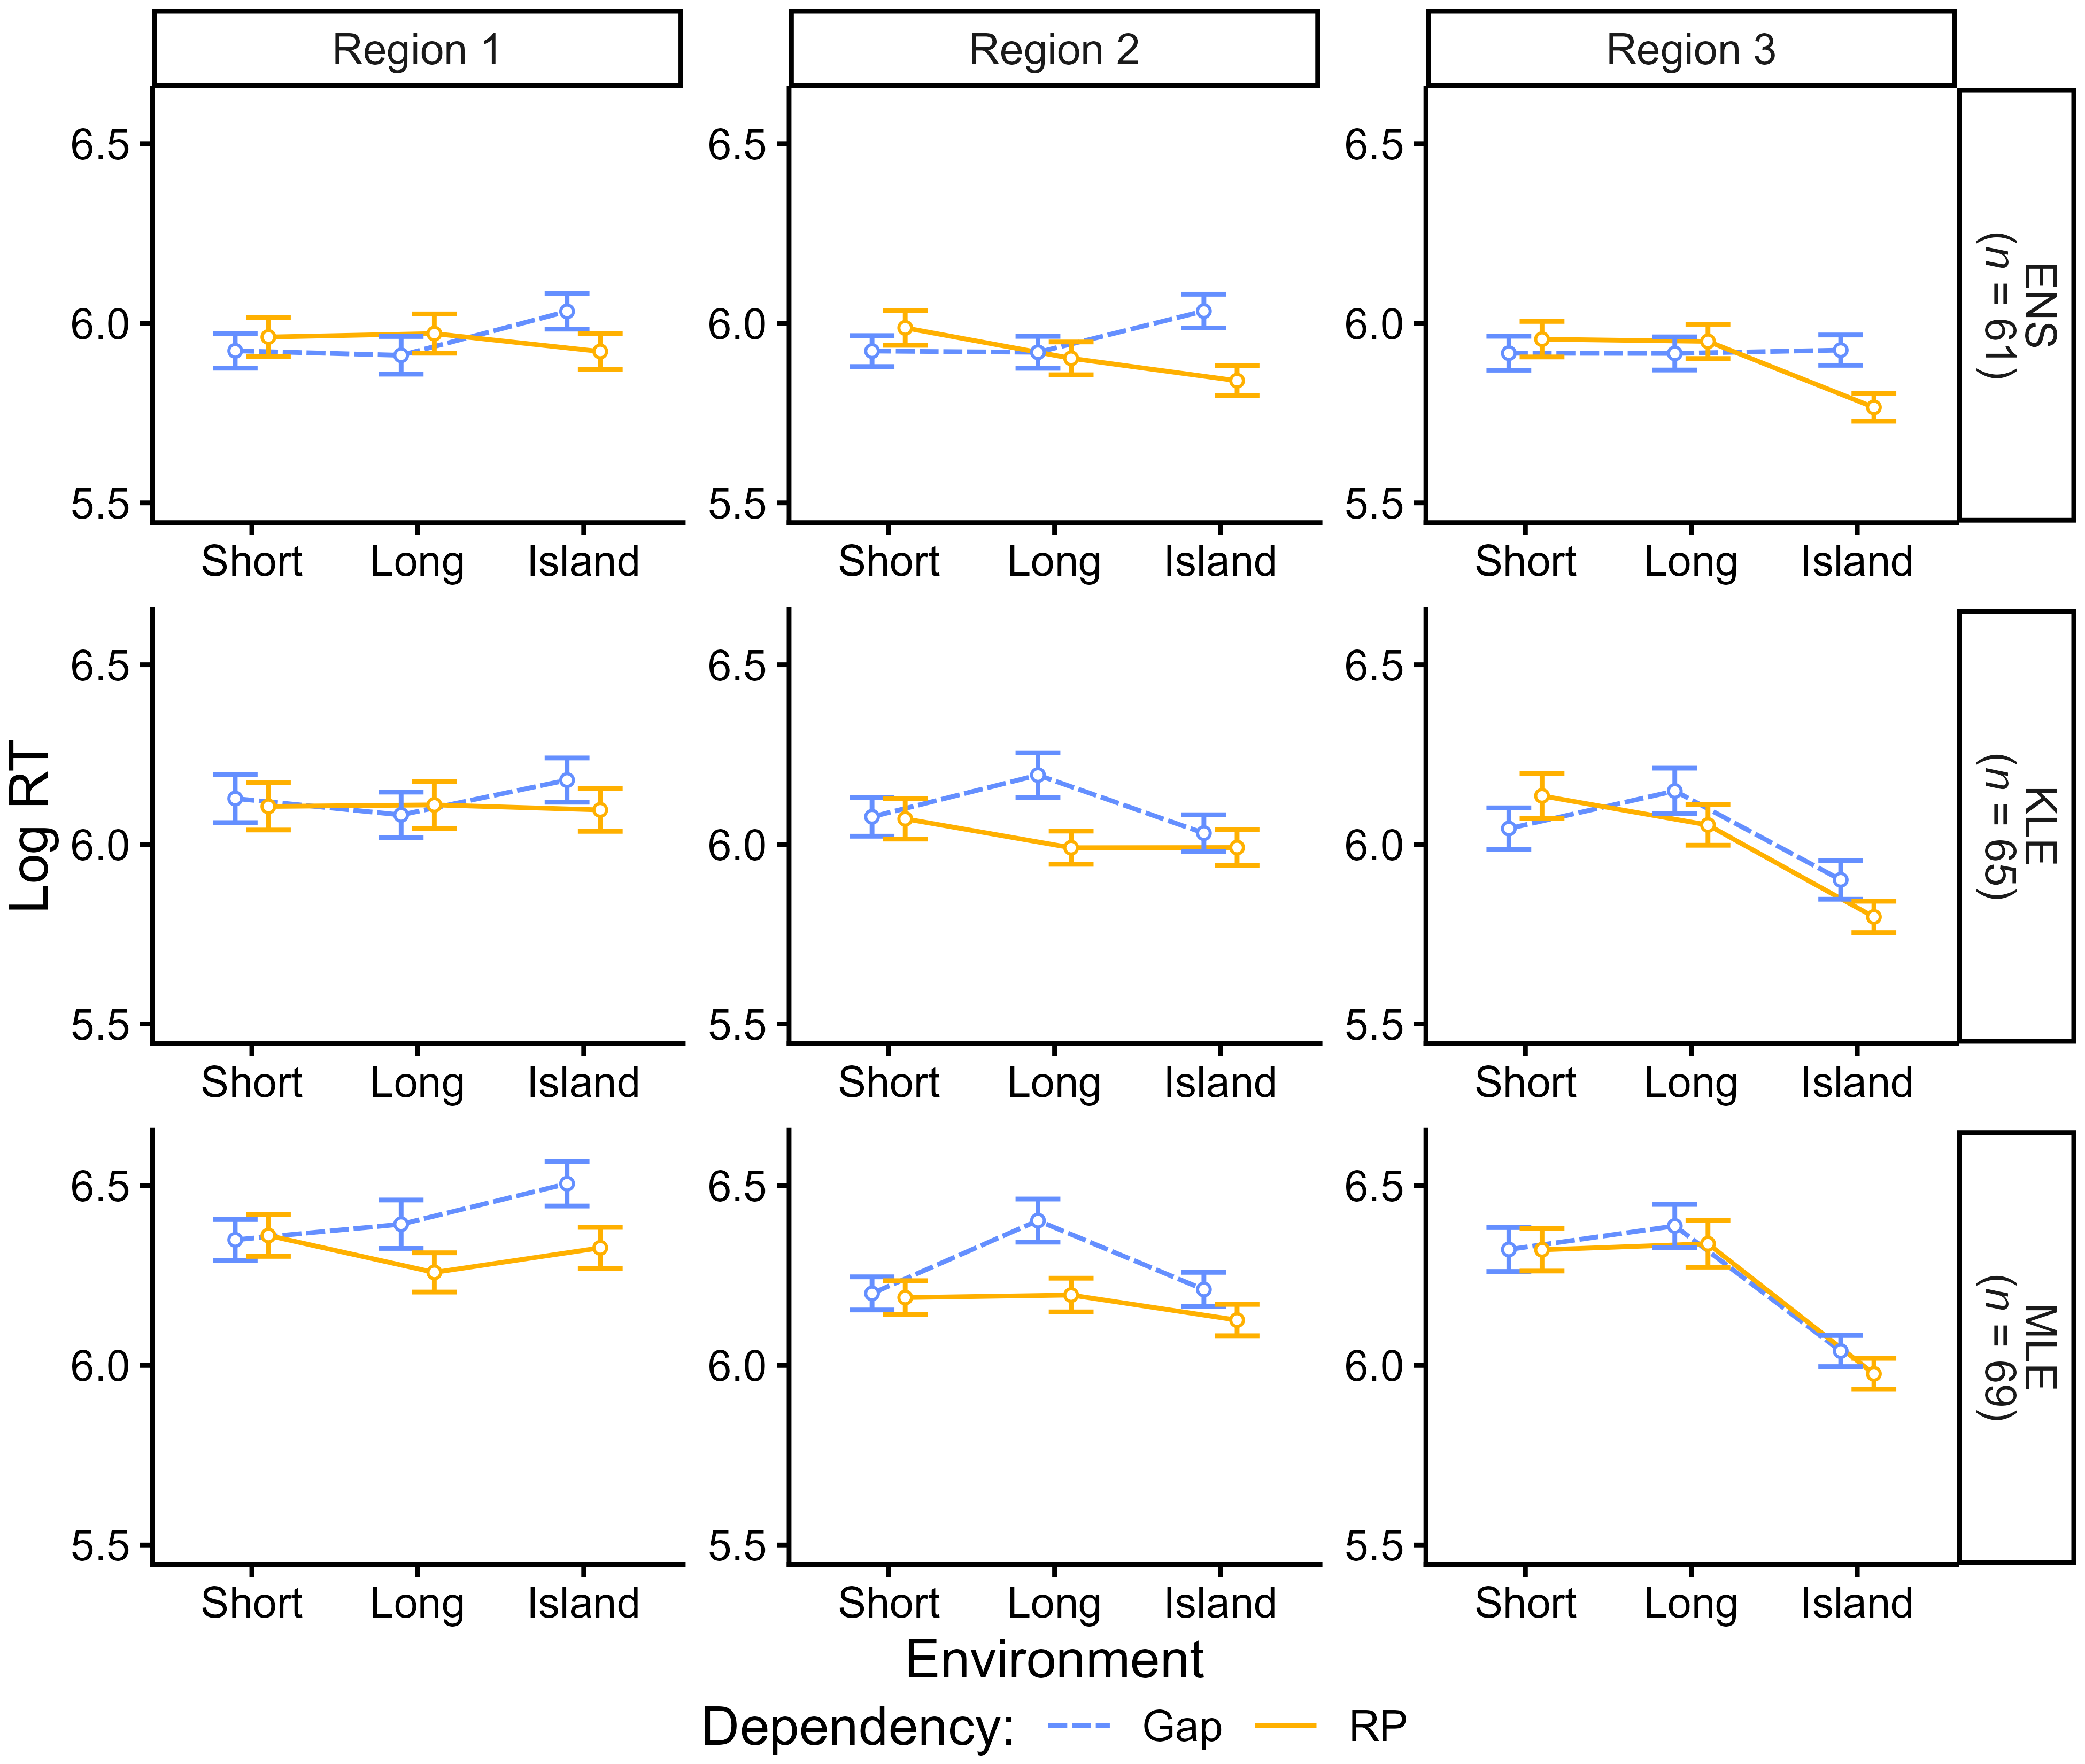
\includegraphics{../analysis/plots/src_spr_logrt2.png}
% \textit{Note}. Error bars are 95\% $CI$s.
% \vspace{-12pt}
% \end{figure}

% ORC Region 1 Model
\begin{table}
\caption{Summary of linear mixed-effects regression model on Region 1 log RTs in the ORC self-paced reading task}\label{tab:app-orc-spr-logrt-r1-model}
\raggedright\setstretch{1}
\begin{tabularx}{\textwidth}{lYYYY}\toprule
Parameter & Estimate~($\hat{\beta}$) & \textit{SE} & $t$ & $p$ \\\midrule
\csvreader[late after line=\\,late after last line=\\\bottomrule]
{../analysis/tables/orc_spr_logrt_region1_model.csv}{}{\csvcoli & \csvcolii & \csvcoliii & \csvcoliv & \csvcolv}
\end{tabularx}
\textit{Note}. Model formula: Log RT \~{} Dependency * Environment * Group + (1 + Dependency + Environment | Participant) + (1 + Dependency + Environment + Group | Item); reference level: Gap + Short + ENS; estimate unit: log-transformed millisecond; intercept: grand mean.
\vspace{-12pt}
\end{table}

% ORC Region 1 Posthoc
\begin{table}
\caption{Post-hoc tests for Region 1 log RTs in the ORC self-paced reading task}\label{tab:app-orc-spr-logrt-r1-posthoc}
\raggedright\setstretch{1}
\begin{tabularx}{\textwidth}{lXXYYYY}\toprule
Group & Environment & Contrast & Estimate~($\hat{\beta}$) & \textit{SE} & $z$ & $p$ \\\midrule
\csvreader[late after line=\\,late after last line=\\\bottomrule]
{../analysis/tables/orc_spr_logrt_region1_posthoc.csv}{}{\csvcoli & \csvcolii & \csvcoliii & \csvcoliv & \csvcolv & \csvcolvi & \csvcolvii}
\end{tabularx}
\textit{Note}. Adjustment to $p$-values done via multiple $t$ method for 9 tests.
\vspace{-12pt}
\end{table}

% ORC REgion 2 Model
\begin{table}
\caption{Summary of linear mixed-effects regression model on Region 2 log RTs in the ORC self-paced reading task}\label{tab:app-orc-spr-logrt-r2-model}
\raggedright\setstretch{1}
\begin{tabularx}{\textwidth}{lYYYY}\toprule
Parameter & Estimate~($\hat{\beta}$) & \textit{SE} & $t$ & $p$ \\\midrule
\csvreader[late after line=\\,late after last line=\\\bottomrule]
{../analysis/tables/orc_spr_logrt_region2_model.csv}{}{\csvcoli & \csvcolii & \csvcoliii & \csvcoliv & \csvcolv}
\end{tabularx}
\textit{Note}. Model formula: Log RT \~{} Dependency * Environment * Group + (1 + Dependency * Environment | Participant) + (1 + Dependency + Environment | Item); reference level: Gap + Short + ENS; estimate unit: log-transformed millisecond; intercept: grand mean.
\vspace{-12pt}
\end{table}

% ORC Region 2 Posthoc
\begin{table}
\caption{Post-hoc tests for Region 2 log RTs in the ORC self-paced reading task}\label{tab:app-orc-spr-logrt-r2-posthoc}
\raggedright\setstretch{1}
\begin{tabularx}{\textwidth}{lXXYYYY}\toprule
Group & Environment & Contrast & Estimate~($\hat{\beta}$) & \textit{SE} & $z$ & $p$ \\\midrule
\csvreader[late after line=\\,late after last line=\\\bottomrule]
{../analysis/tables/orc_spr_logrt_region2_posthoc.csv}{}{\csvcoli & \csvcolii & \csvcoliii & \csvcoliv & \csvcolv & \csvcolvi & \csvcolvii}
\end{tabularx}
\textit{Note}. Adjustment to $p$-values done via multiple $t$ method for 9 tests.
\vspace{-12pt}
\end{table}

% ORC Region 3 Model
\begin{table}
\caption{Summary of linear mixed-effects regression model on Region 3 log RTs in the ORC self-paced reading task}\label{tab:app-orc-spr-logrt-r3-model}
\raggedright\setstretch{1}
\begin{tabularx}{\textwidth}{lYYYY}\toprule
Parameter & Estimate~($\hat{\beta}$) & \textit{SE} & $t$ & $p$ \\\midrule
\csvreader[late after line=\\,late after last line=\\\bottomrule]
{../analysis/tables/orc_spr_logrt_region3_model.csv}{}{\csvcoli & \csvcolii & \csvcoliii & \csvcoliv & \csvcolv}
\end{tabularx}
\textit{Note}. Model formula: Log RT \~{} Dependency * Environment * Group + (1 + Dependency * Environment | Participant) + (1 + Dependency + Environment + Group | Item); reference level: Gap + Short + ENS; estimate unit: log-transformed millisecond; intercept: grand mean.
\vspace{-12pt}
\end{table}

% ORC Region 3 Posthoc
\begin{table}
\caption{Post-hoc tests for Region 3 log RTs in the ORC self-paced reading task}\label{tab:app-orc-spr-logrt-r3-posthoc}
\raggedright\setstretch{1}
\begin{tabularx}{\textwidth}{lXXYYYY}\toprule
Group & Environment & Contrast & Estimate~($\hat{\beta}$) & \textit{SE} & $z$ & $p$ \\\midrule
\csvreader[late after line=\\,late after last line=\\\bottomrule]
{../analysis/tables/orc_spr_logrt_region3_posthoc.csv}{}{\csvcoli & \csvcolii & \csvcoliii & \csvcoliv & \csvcolv & \csvcolvi & \csvcolvii}
\end{tabularx}
\textit{Note}. Adjustment to $p$-values done via multiple $t$ method for 9 tests.
\vspace{-12pt}
\end{table}

% SRC Region 1 Model
\begin{table}
\caption{Summary of linear mixed-effects regression model on Region 1 log RTs in the SRC self-paced reading task}\label{tab:app-src-spr-logrt-r1-model}
\raggedright\setstretch{1}
\begin{tabularx}{\textwidth}{lYYYY}\toprule
Parameter & Estimate~($\hat{\beta}$) & \textit{SE} & $t$ & $p$ \\\midrule
\csvreader[late after line=\\,late after last line=\\\bottomrule]
{../analysis/tables/src_spr_logrt_region1_model.csv}{}{\csvcoli & \csvcolii & \csvcoliii & \csvcoliv & \csvcolv}
\end{tabularx}
\textit{Note}. Model formula: Log RT \~{} Dependency * Environment * Group + (1 | Participant) + (1 + Dependency + Environment + Group | Item); reference level: Gap + Short + ENS; estimate unit: log-transformed millisecond; intercept: grand mean.
\vspace{-12pt}
\end{table}

% SRC Region 1 Posthoc
\begin{table}
\caption{Post-hoc tests for Region 1 log RTs in the SRC self-paced reading task}\label{tab:app-src-spr-logrt-r1-posthoc}
\raggedright\setstretch{1}
\begin{tabularx}{\textwidth}{lXXYYYY}\toprule
Group & Environment & Contrast & Estimate~($\hat{\beta}$) & \textit{SE} & $z$ & $p$ \\\midrule
\csvreader[late after line=\\,late after last line=\\\bottomrule]
{../analysis/tables/src_spr_logrt_region1_posthoc.csv}{}{\csvcoli & \csvcolii & \csvcoliii & \csvcoliv & \csvcolv & \csvcolvi & \csvcolvii}
\end{tabularx}
\textit{Note}. Adjustment to $p$-values done via multiple $t$ method for 9 tests.
\vspace{-12pt}
\end{table}

% SRC Region 2 Model
\begin{table}
\caption{Summary of linear mixed-effects regression model on Region 2 log RTs in the SRC self-paced reading task}\label{tab:app-src-spr-logrt-r2-model}
\raggedright\setstretch{1}
\begin{tabularx}{\textwidth}{lYYYY}\toprule
Parameter & Estimate~($\hat{\beta}$) & \textit{SE} & $t$ & $p$ \\\midrule
\csvreader[late after line=\\,late after last line=\\\bottomrule]
{../analysis/tables/src_spr_logrt_region2_model.csv}{}{\csvcoli & \csvcolii & \csvcoliii & \csvcoliv & \csvcolv}
\end{tabularx}
\textit{Note}. Model formula: Log RT \~{} Dependency * Environment * Group + (1 + Dependency * Environment | Participant) + (1 + Dependency + Environment + Group | Item); reference level: Gap + Short + ENS; estimate unit: log-transformed millisecond; intercept: grand mean.
\vspace{-12pt}
\end{table}

% SRC Region 2 Posthoc
\begin{table}
\caption{Post-hoc tests for Region 2 log RTs in the SRC self-paced reading task}\label{tab:app-src-spr-logrt-r2-posthoc}
\raggedright\setstretch{1}
\begin{tabularx}{\textwidth}{lXXYYYY}\toprule
Group & Environment & Contrast & Estimate~($\hat{\beta}$) & \textit{SE} & $z$ & $p$ \\\midrule
\csvreader[late after line=\\,late after last line=\\\bottomrule]
{../analysis/tables/src_spr_logrt_region2_posthoc.csv}{}{\csvcoli & \csvcolii & \csvcoliii & \csvcoliv & \csvcolv & \csvcolvi & \csvcolvii}
\end{tabularx}
\textit{Note}. Adjustment to $p$-values done via multiple $t$ method for 9 tests.
\vspace{-12pt}
\end{table}

% SRC Region 3 Model
\begin{table}
\caption{Summary of linear mixed-effects regression model on Region 3 log RTs in the SRC self-paced reading task}\label{tab:app-src-spr-logrt-r3-model}
\raggedright\setstretch{1}
\begin{tabularx}{\textwidth}{lYYYY}\toprule
Parameter & Estimate~($\hat{\beta}$) & \textit{SE} & $t$ & $p$ \\\midrule
\csvreader[late after line=\\,late after last line=\\\bottomrule]
{../analysis/tables/src_spr_logrt_region3_model.csv}{}{\csvcoli & \csvcolii & \csvcoliii & \csvcoliv & \csvcolv}
\end{tabularx}
\textit{Note}. Model formula: Log RT \~{} Dependency * Environment * Group + (1 + Dependency * Environment | Participant) + (1 + Dependency + Environment + Group | Item); reference level: Gap + Short + ENS; estimate unit: log-transformed millisecond; intercept: grand mean.
\vspace{-12pt}
\end{table}

% SRC Region 3 Posthoc
\begin{table}
\caption{Post-hoc tests for Region 3 log RTs in the SRC self-paced reading task}\label{tab:app-src-spr-logrt-r3-posthoc}
\raggedright\setstretch{1}
\begin{tabularx}{\textwidth}{lXXYYYY}\toprule
Group & Environment & Contrast & Estimate~($\hat{\beta}$) & \textit{SE} & $z$ & $p$ \\\midrule
\csvreader[late after line=\\,late after last line=\\\bottomrule]
{../analysis/tables/src_spr_logrt_region3_posthoc.csv}{}{\csvcoli & \csvcolii & \csvcoliii & \csvcoliv & \csvcolv & \csvcolvi & \csvcolvii}
\end{tabularx}
\textit{Note}. Adjustment to $p$-values done via multiple $t$ method for 9 tests.
\end{table}

%========================================================%
\section{L2 proficiency effects for RTs at the regions of interest}\label{app-spr-logrt-proficiency}
%========================================================%

% ORC and SRC D-scores
\begin{table}
\caption{Difference scores for the [RP~−~Gap] log RT contrast in the ORC and SRC datasets}\label{tab:app-spr-dscore}
\raggedright\setstretch{1}
\begin{tabularx}{\linewidth}{lYYY}\toprule
Study & Region 1 & Region 2 & Region 3 \\\midrule
ORC & −0.063 & −0.055 & −0.032 \\
SRC & −0.044 & −0.078 & −0.034 \\\bottomrule
\end{tabularx}
\vspace{-12pt}
\end{table}

% ORC Figure
% \begin{figure}
% \caption{Relationship between L2 proficiency and log RTs in the ORC self-paced reading task} \label{fig:app-orc-spr-rt-proficiency}
% \raggedright\setstretch{1}
% 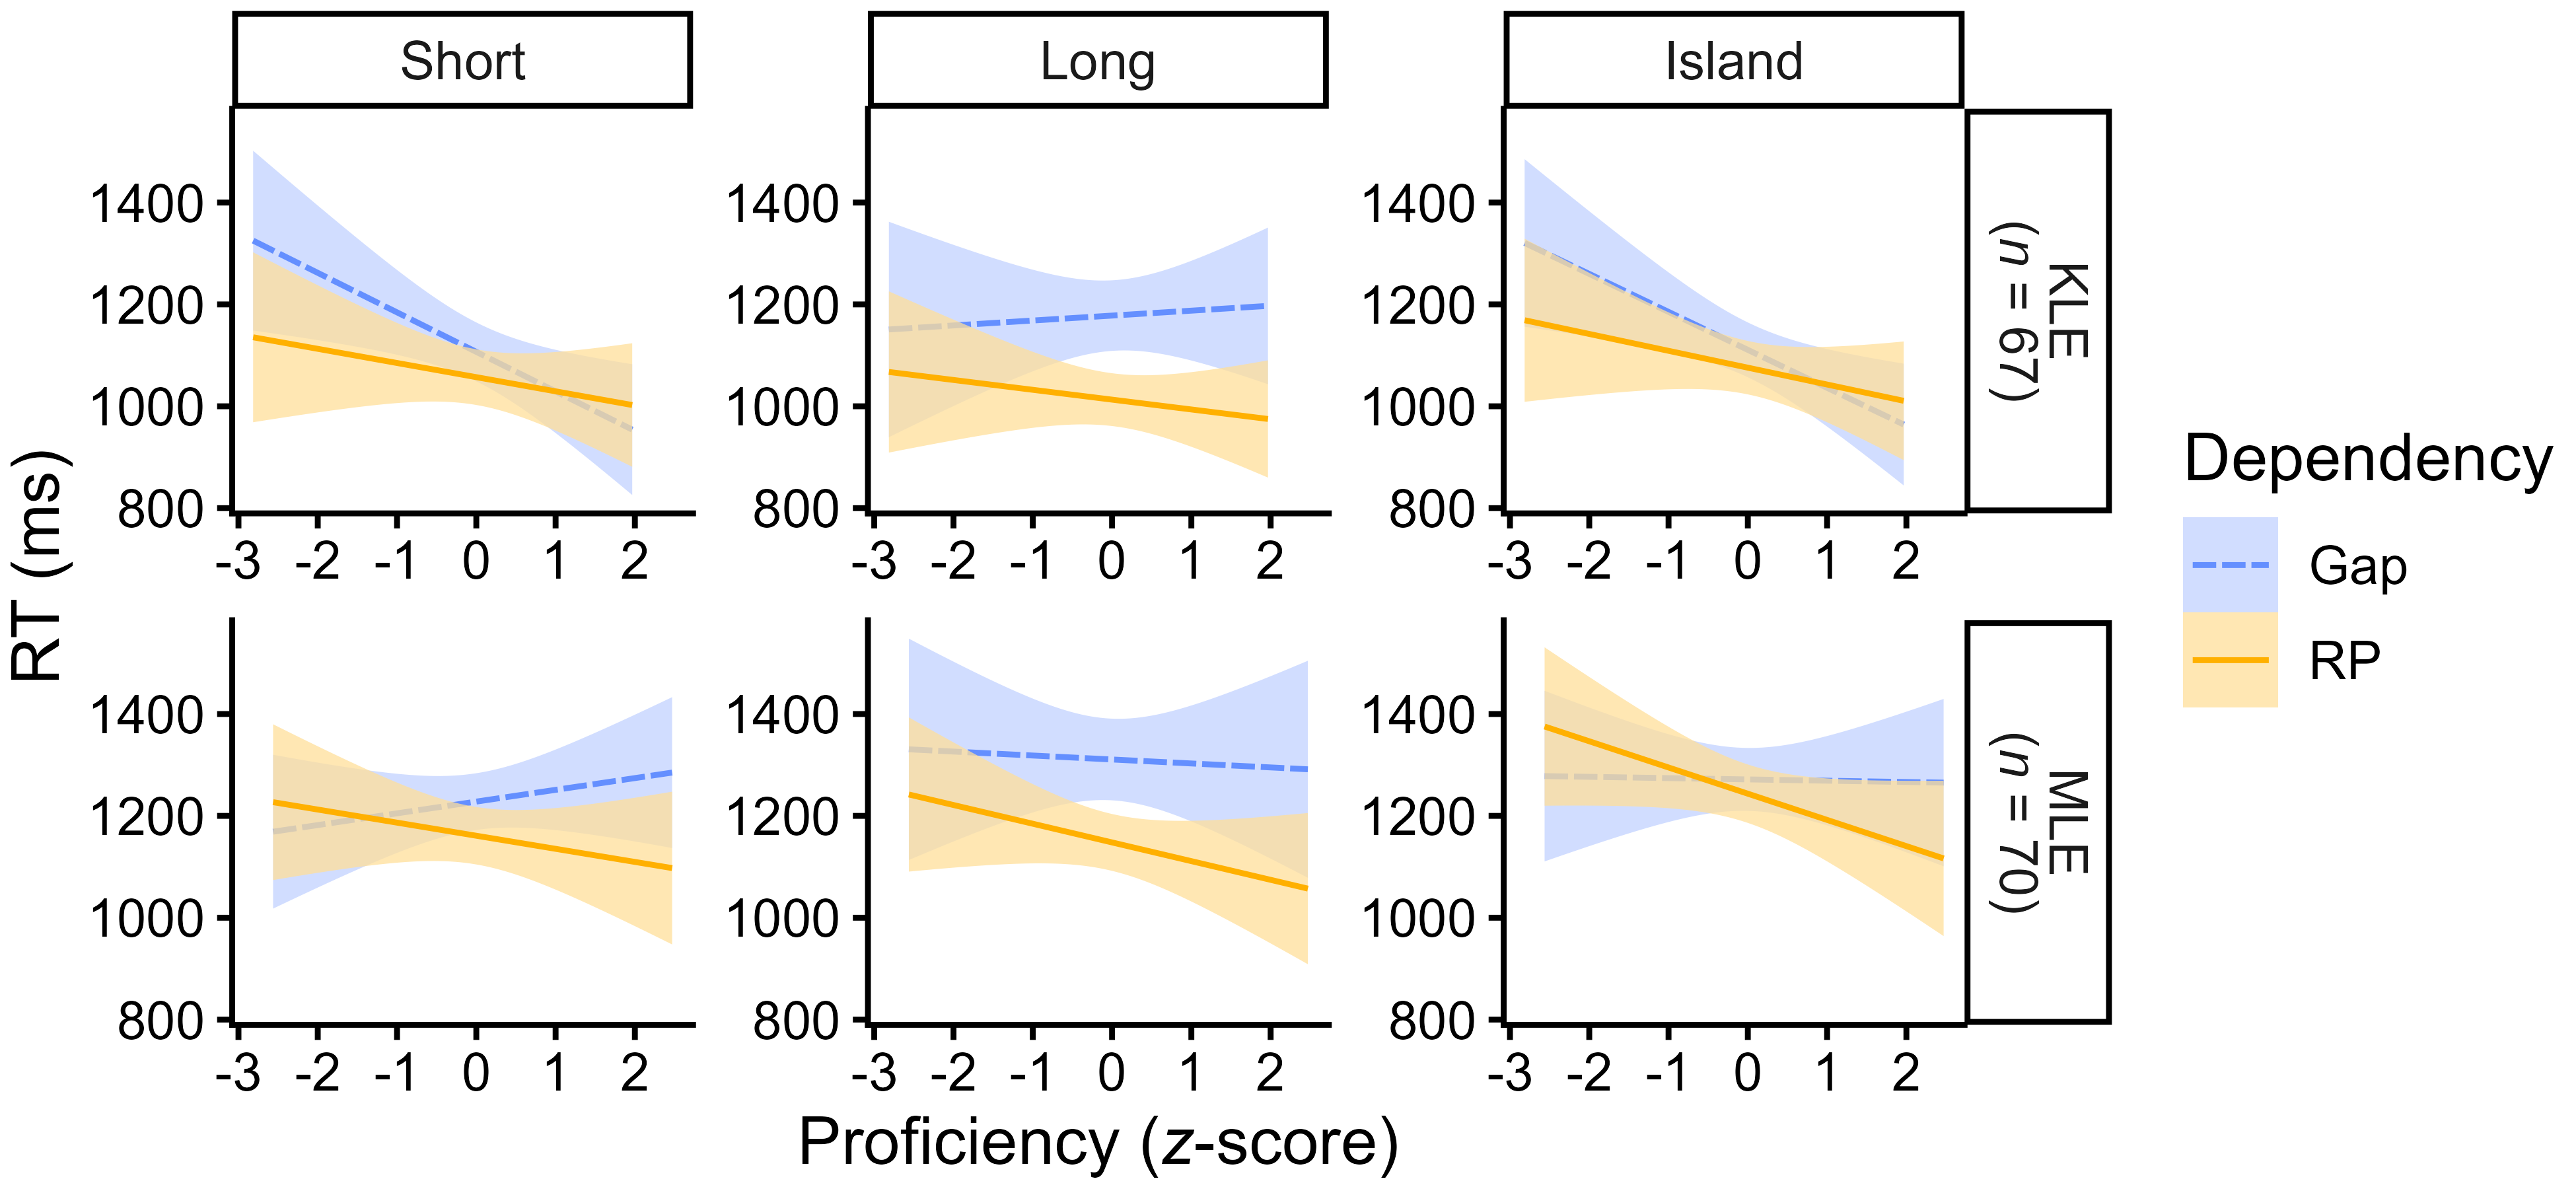
\includegraphics{../analysis/plots/orc_spr_rt_proficiency.png}
% \textit{Note}. Shading indicates 95\% $CI$s.
% \vspace{-12pt}
% \end{figure}

% SRC Figure
% \begin{figure}
% \caption{Relationship between L2 proficiency and log RTs in the SRC self-paced reading task} \label{fig:app-src-spr-rt-proficiency}
% \raggedright\setstretch{1}
% 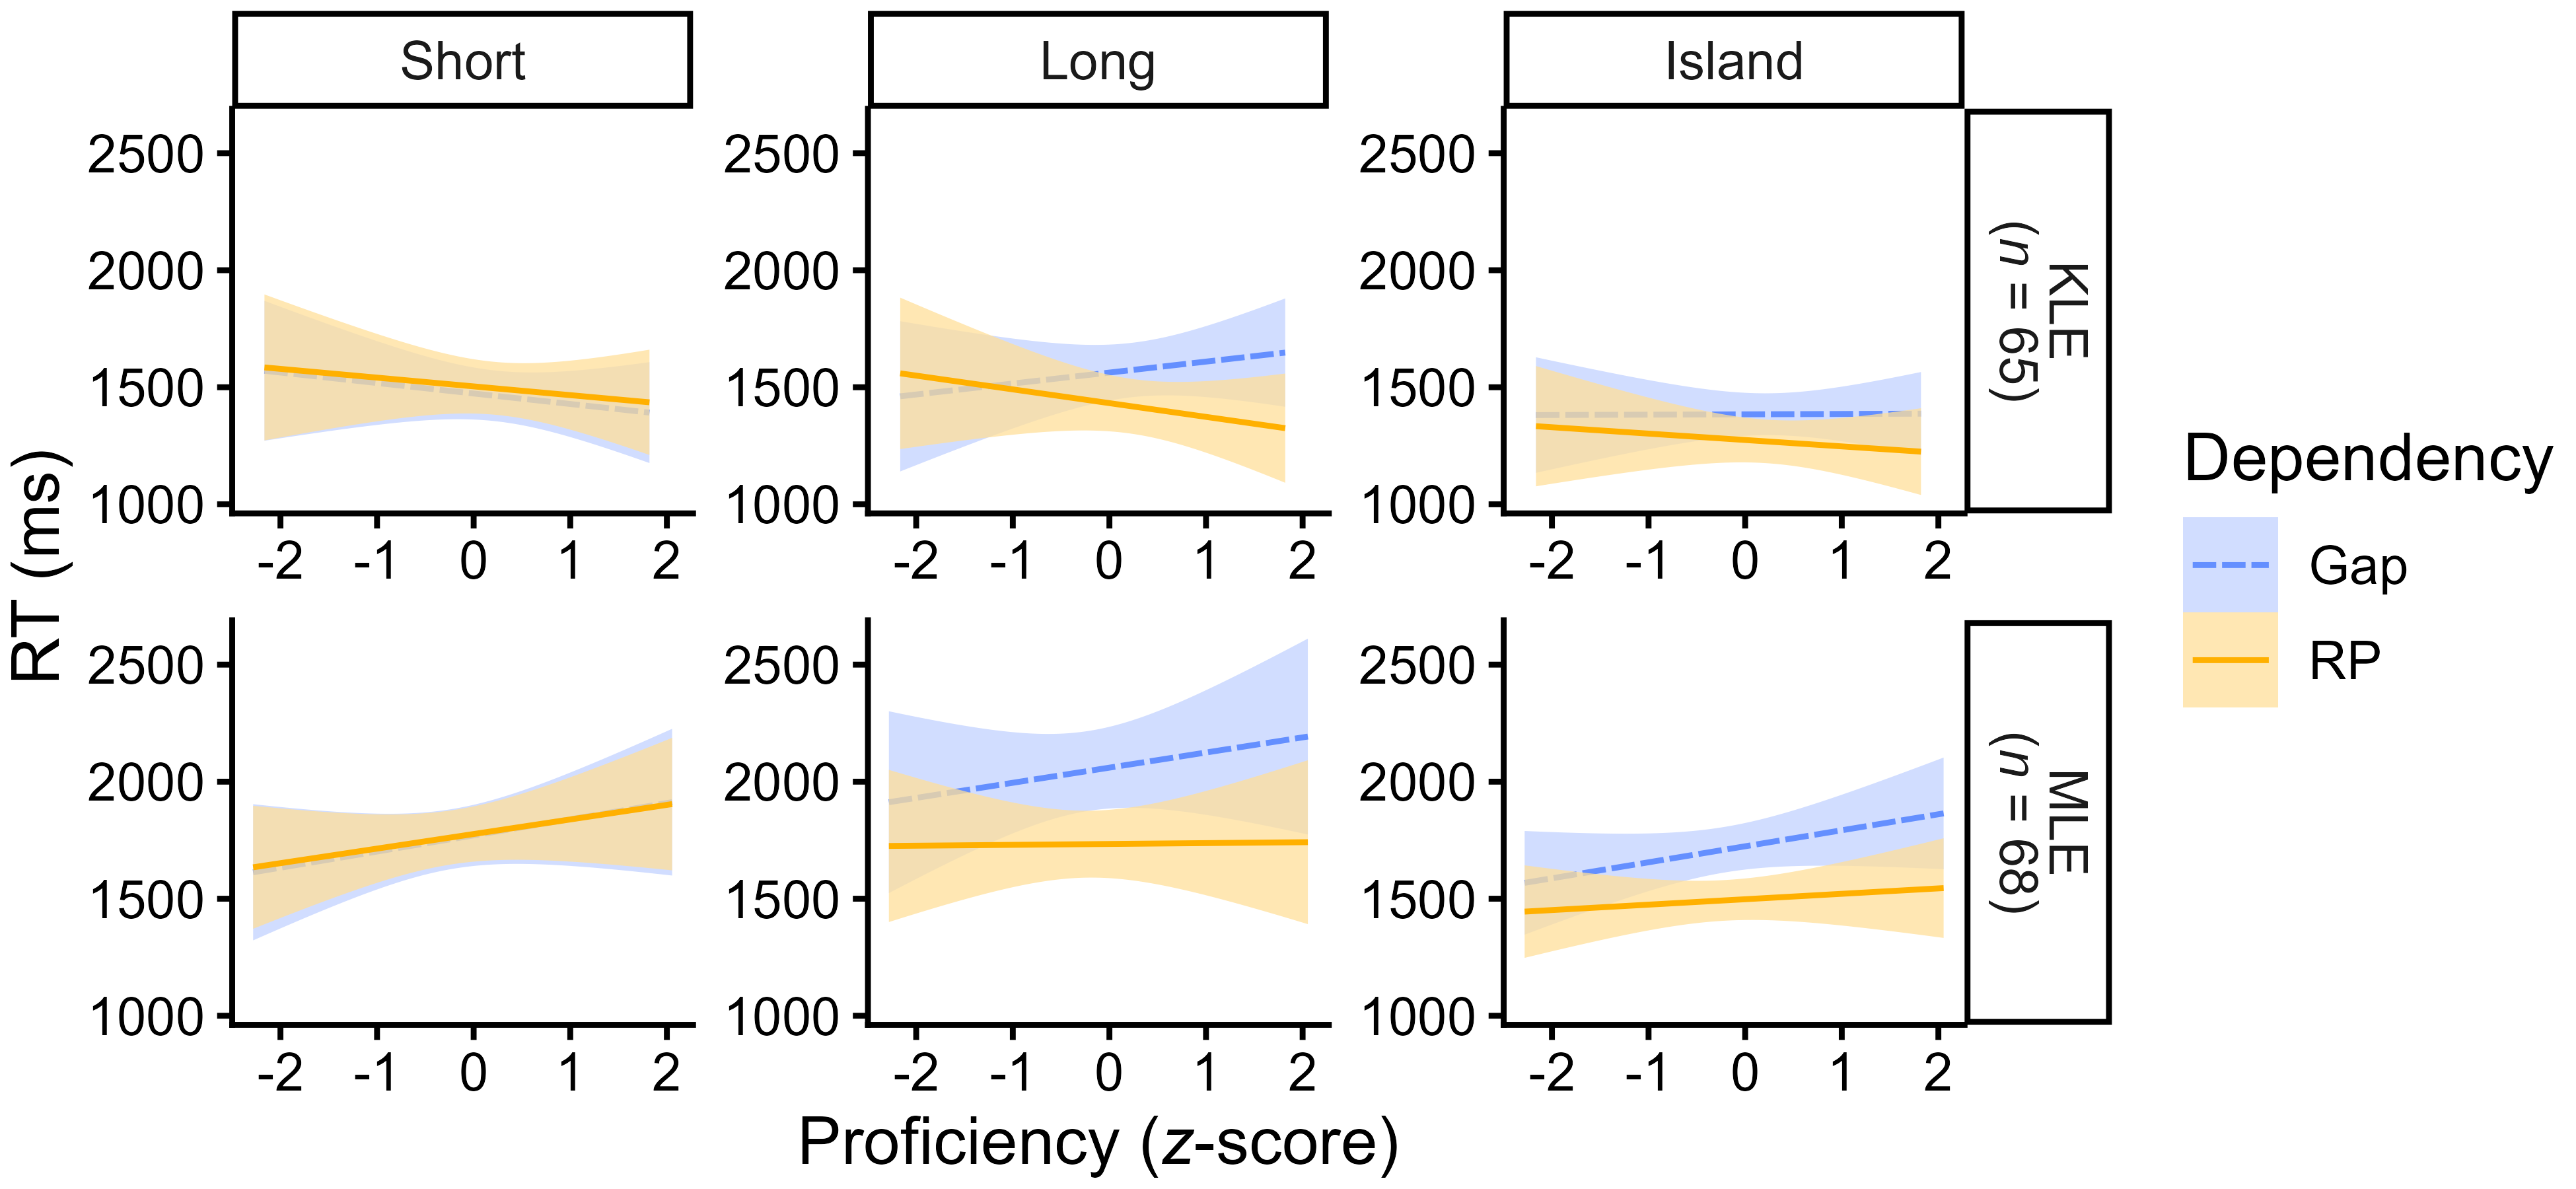
\includegraphics{../analysis/plots/src_spr_rt_proficiency.png}
% \textit{Note}. Shading indicates 95\% $CI$s.
% \vspace{-12pt}
% \end{figure}

% ORC Model
\begin{table}
\caption{Summary of linear mixed-effects regression model for L2 proficiency effects on Region~1 log RTs in the ORC self-paced reading task}\label{tab:app-orc-spr-logrt-proficiency-model}
\raggedright\setstretch{1}
\begin{tabularx}{\textwidth}{lrYYY}\toprule
Parameter & Estimate~($\hat{\beta}$) & \textit{SE} & $z$ & $p$ \\\midrule
\csvreader[late after line=\\,late after last line=\\\bottomrule]
{../analysis/tables/orc_spr_logrt_proficiency_model.csv}{}{\csvcoli & \csvcolii & \csvcoliii & \csvcoliv & \csvcolv}
\end{tabularx}
\textit{Note}. Model formula: Log RT \~{} Dependency * Environment * Group * Proficiency + (1 + Dependency * Environment | Participant) + (1 + Dependency + Environment + Group | Item); reference level: Gap + Short + KLE; estimate unit: log-transformed millisecond; intercept: grand mean.
\vspace{-12pt}
\end{table}

% ORC Posthoc
\begin{table}
\caption{Post-hoc tests for L2 proficiency effects on Region~1 log RTs in the ORC self-paced reading task}\label{tab:app-orc-spr-logrt-proficiency-posthoc}
\raggedright\setstretch{1}
\begin{tabularx}{\textwidth}{lXXYYYY}\toprule
Group & Environment & Contrast & Estimate~($\hat{\beta}$) & \textit{SE} & $z$ & $p$ \\\midrule
\csvreader[late after line=\\,late after last line=\\\bottomrule]
{../analysis/tables/orc_spr_logrt_proficiency_posthoc.csv}{}{\csvcoli & \csvcolii & \csvcoliii & \csvcoliv & \csvcolv & \csvcolvi & \csvcolvii}
\end{tabularx}
\textit{Note}. Adjustment to $p$-values done via multiple $t$ method for 6 tests.
\vspace{-12pt}
\end{table}

% SRC Model
\begin{table}
\caption{Summary of linear mixed-effects regression model for L2 proficiency effects on Region~2 log RTs in the SRC self-paced reading task}\label{tab:app-src-spr-logrt-proficiency-model}
\raggedright\setstretch{1}
\begin{tabularx}{\textwidth}{lrYYY}\toprule
Parameter & Estimate~($\hat{\beta}$) & \textit{SE} & $z$ & $p$ \\\midrule
\csvreader[late after line=\\,late after last line=\\\bottomrule]
{../analysis/tables/src_spr_logrt_proficiency_model.csv}{}{\csvcoli & \csvcolii & \csvcoliii & \csvcoliv & \csvcolv}
\end{tabularx}
\textit{Note}. Model formula: Log RT \~{} Dependency * Environment * Group * Proficiency + (1 + Dependency + Environment | Participant) + (1 + Dependency + Environment + Group | Item); reference level: Gap + Short + KLE; estimate unit: log-transformed millisecond; intercept: grand mean.
\vspace{-12pt}
\end{table}

% SRC Posthoc
\begin{table}
\caption{Post-hoc tests for L2 proficiency effects on Region~2 log RTs in the SRC self-paced reading task}\label{tab:app-src-spr-logrt-proficiency-posthoc}
\raggedright\setstretch{1}
\begin{tabularx}{\textwidth}{lXXYYYY}\toprule
Group & Environment & Contrast & Estimate~($\hat{\beta}$) & \textit{SE} & $z$ & $p$ \\\midrule
\csvreader[late after line=\\,late after last line=\\\bottomrule]
{../analysis/tables/src_spr_logrt_proficiency_posthoc.csv}{}{\csvcoli & \csvcolii & \csvcoliii & \csvcoliv & \csvcolv & \csvcolvi & \csvcolvii}
\end{tabularx}
\textit{Note}. Adjustment to $p$-values done via multiple $t$ method for 6 tests.
\end{table}

%========================================================%
\section{Comprehension-question accuracy}\label{app-spr-accuracy}
%========================================================%

% ORC Means
% \DTLloaddb{dt-spr-accuracy}{../analysis/tables/spr_accuracy.csv}
% \ExplSyntaxOn
% \tl_clear:N \tblrbody
% \tl_build_begin:N \tblrbody
% \DTLforeach[\equal{\study}{ORC}]{dt-spr-accuracy}{\study=study,\coli=Group,\colii=Environment,\coliii=Dependency,\coliv=Mean,\colv=$CI$}{\tl_build_put_right:Ne \tblrbody {\exp_not:V \coli & \exp_not:V \colii & \exp_not:V \coliii & \exp_not:V \coliv & \exp_not:V \colv\\}}
% \tl_build_end:N \tblrbody
% \ExplSyntaxOff
% \begin{longtblr}[caption={Mean comprehension-question accuracy in the ORC self-paced reading task}, label={tblr:app-orc-spr-accuracy}, expand=\tblrbody]{colspec={XXXX[r]X[r]}}\toprule
% Group & Environment & Dependency & Mean & 95\% \textit{CI}\\\midrule
% \tblrbody\bottomrule
% \end{longtblr}
% \vspace{-12pt}

% SRC Means
% \ExplSyntaxOn
% \tl_clear:N \tblrbody
% \tl_build_begin:N \tblrbody
% \DTLforeach[\equal{\study}{SRC}]{dt-spr-accuracy}{\study=study,\coli=Group,\colii=Environment,\coliii=Dependency,\coliv=Mean,\colv=$CI$}{\tl_build_put_right:Ne \tblrbody {\exp_not:V \coli & \exp_not:V \colii & \exp_not:V \coliii & \exp_not:V \coliv & \exp_not:V \colv\\}}
% \tl_build_end:N \tblrbody
% \ExplSyntaxOff
% \begin{longtblr}[caption={Mean comprehension-question accuracy in the SRC self-paced reading task}, label={tblr:app-src-spr-accuracy}, expand=\tblrbody]{colspec={XXXX[r]X[r]}}\toprule
% Group & Environment & Dependency & Mean & 95\% \textit{CI}\\\midrule
% \tblrbody\bottomrule
% \end{longtblr}
% \vspace{-12pt}

% ORC Figure
% \begin{figure}
% \caption{Mean comprehension-question accuracy in the ORC self-paced reading task} \label{fig:app-orc-spr-accuracy}
% \raggedright\setstretch{1}
% 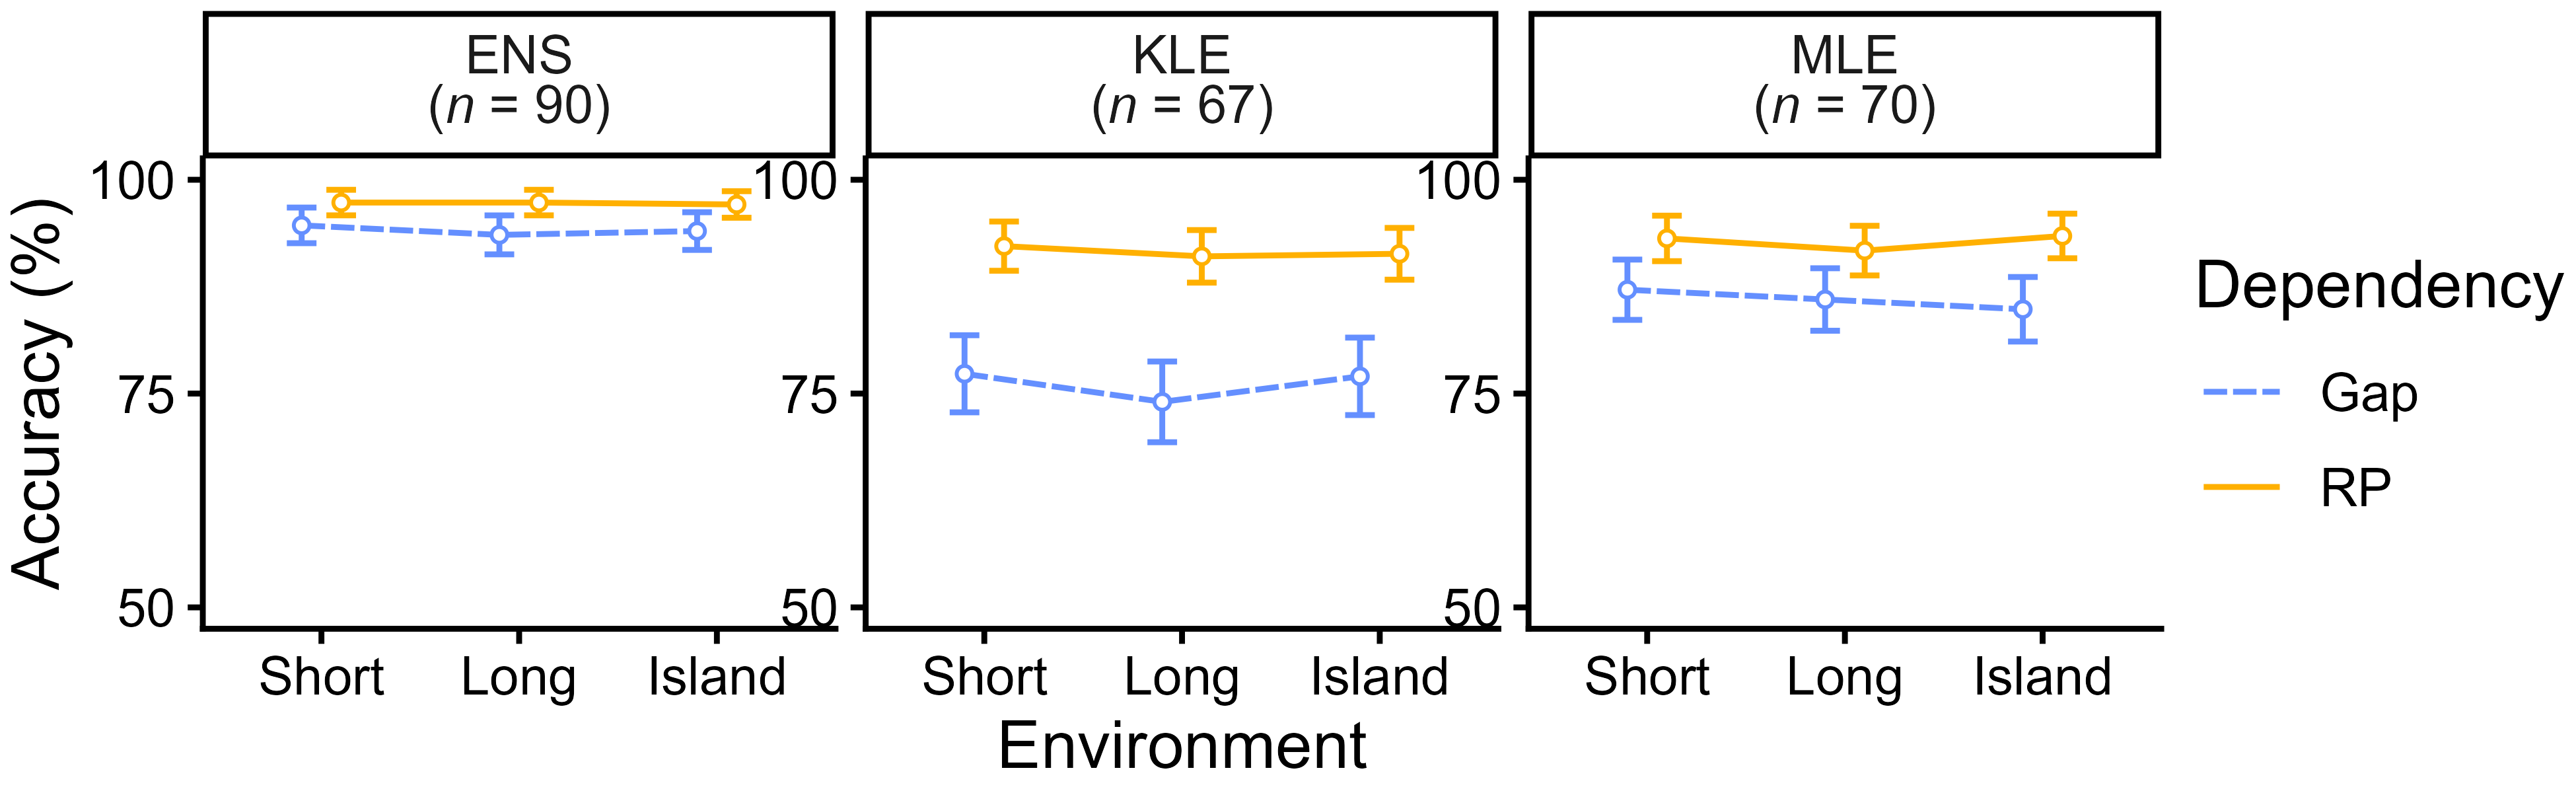
\includegraphics{../analysis/plots/orc_spr_accuracy.png}
% \textit{Note}. Error bars are 95\% $CI$s.
% \vspace{-12pt}
% \end{figure}

% SRC Figure
% \begin{figure}
% \caption{Mean comprehension-question accuracy in the SRC self-paced reading task} \label{fig:app-src-spr-accuracy}
% \raggedright\setstretch{1}
% 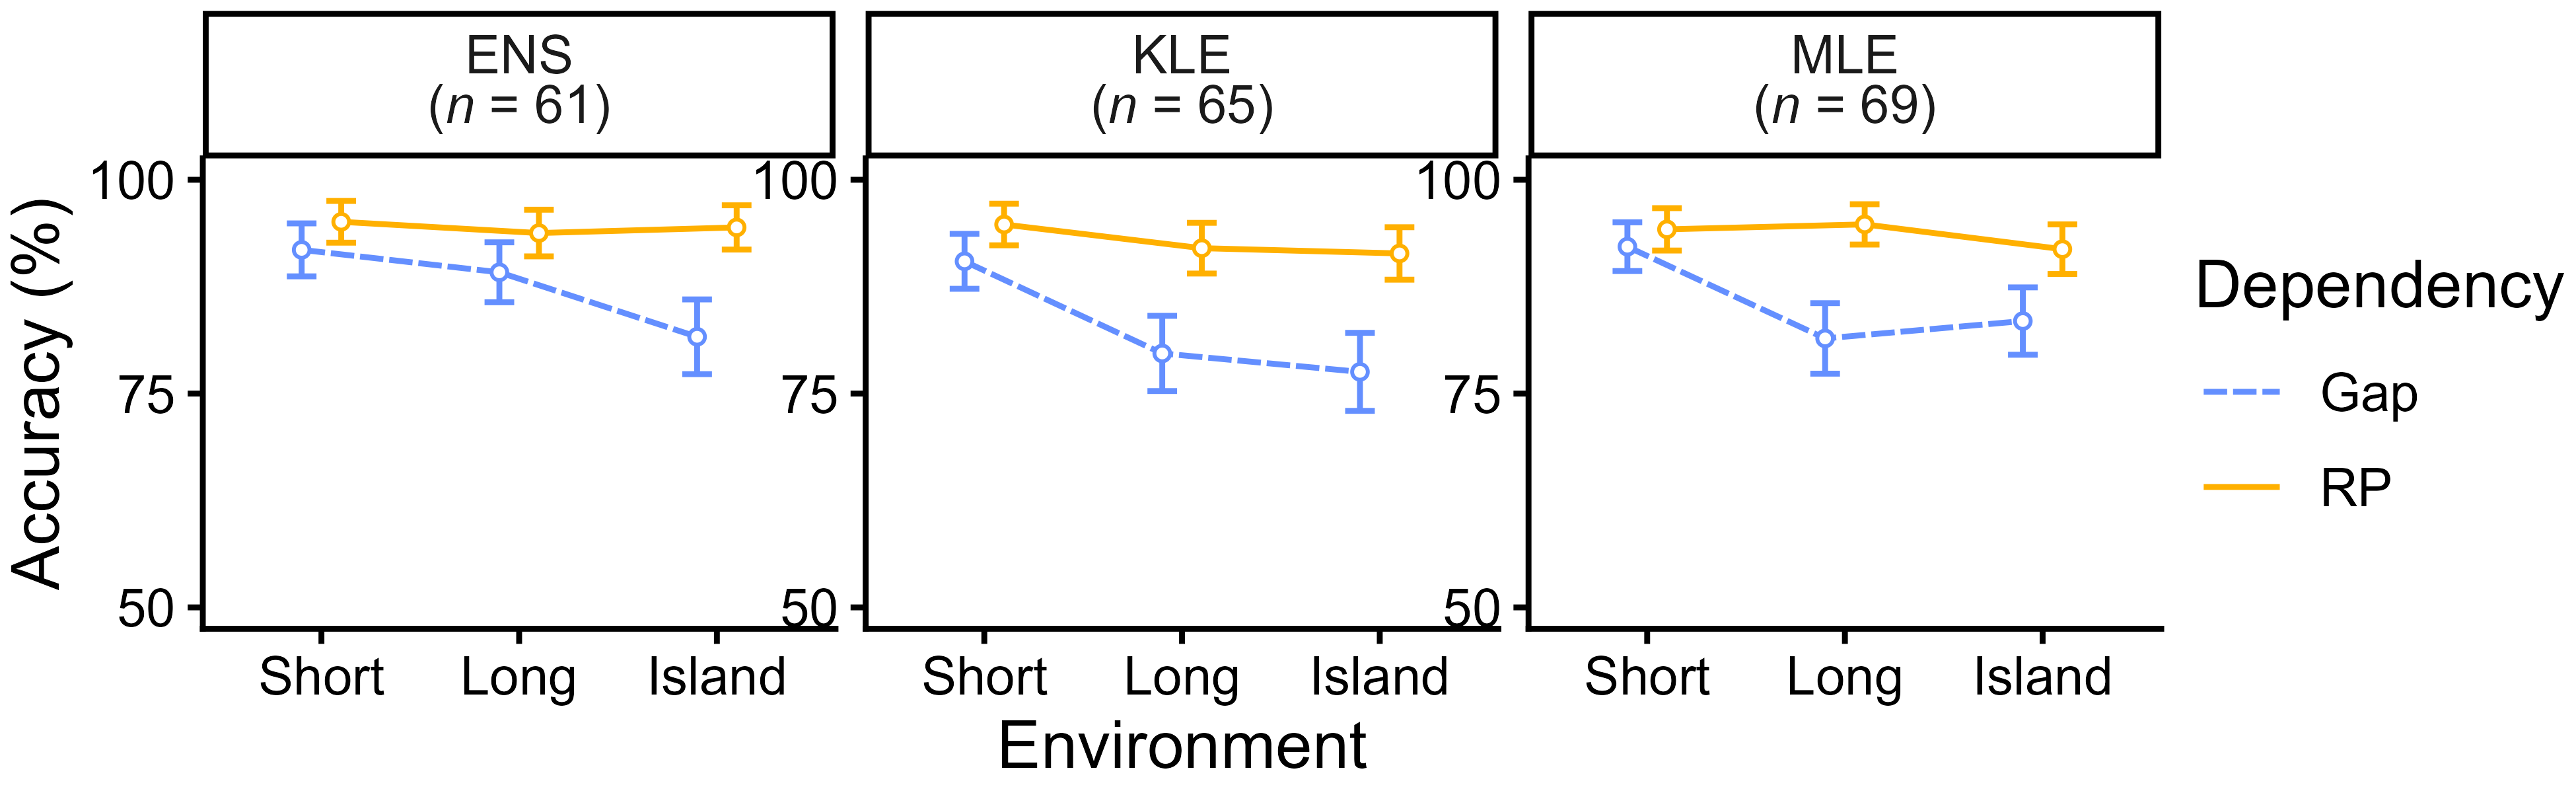
\includegraphics{../analysis/plots/src_spr_accuracy.png}
% \textit{Note}. Error bars are 95\% $CI$s.
% \vspace{-12pt}
% \end{figure}

% ORC Model
\begin{table}
\caption{Summary of mixed-effects logistic regression model on comprehension-question accuracy in the ORC self-paced reading task}\label{tab:app-orc-spr-accuracy-model}
\raggedright\setstretch{1}
\begin{tabularx}{\textwidth}{lrYYY}\toprule
Parameter & Estimate~($\hat{\beta}$) & \textit{SE} & $z$ & $p$ \\\midrule
\csvreader[late after line=\\,late after last line=\\\bottomrule]
{../analysis/tables/orc_spr_accuracy_model.csv}{}{\csvcoli & \csvcolii & \csvcoliii & \csvcoliv & \csvcolv}
\end{tabularx}
\textit{Note}. Model formula: Accuracy \~{} Dependency * Environment * Group + (1 + Dependency + Environment | Participant) + (1 + Dependency + Environment + Group | Item); reference level: Gap + Short + ENS; estimate unit: logit; intercept: grand mean.
\vspace{-12pt}
\end{table}

% ORC Posthoc
\begin{table}
\caption{Post-hoc tests for comprehension-question accuracy in the ORC self-paced reading task}\label{tab:app-orc-spr-accuracy-posthoc}
\raggedright\setstretch{1}
\begin{tabularx}{\textwidth}{lXXYYYY}\toprule
Group & Environment & Contrast & Estimate~($\hat{\beta}$) & \textit{SE} & $z$ & $p$ \\\midrule
\csvreader[late after line=\\,late after last line=\\\bottomrule]
{../analysis/tables/orc_spr_accuracy_posthoc.csv}{}{\csvcoli & \csvcolii & \csvcoliii & \csvcoliv & \csvcolv & \csvcolvi & \csvcolvii}
\end{tabularx}
\textit{Note}. Adjustment to $p$-values done via multiple $t$ method for 9 tests.
\vspace{-12pt}
\end{table}

% SRC Model
\begin{table}
\caption{Summary of mixed-effects logistic regression model on comprehension-question accuracy in the SRC self-paced reading task}\label{tab:app-src-spr-accuracy-model}
\raggedright\setstretch{1}
\begin{tabularx}{\textwidth}{lrYYY}\toprule
Parameter & Estimate~($\hat{\beta}$) & \textit{SE} & $z$ & $p$ \\\midrule
\csvreader[late after line=\\,late after last line=\\\bottomrule]
{../analysis/tables/src_spr_accuracy_model.csv}{}{\csvcoli & \csvcolii & \csvcoliii & \csvcoliv & \csvcolv}
\end{tabularx}
\textit{Note}. Model formula: Accuracy \~{} Dependency * Environment * Group + (1 + Dependency + Environment | Participant) + (1 + Dependency + Environment + Group | Item); reference level: Gap + Short + ENS; estimate unit: logit; intercept: grand mean.
\vspace{-12pt}
\end{table}

% SRC Posthoc
\begin{table}
\caption{Post-hoc tests for comprehension-question accuracy in the SRC self-paced reading task}\label{tab:app-src-spr-accuracy-posthoc}
\raggedright\setstretch{1}
\begin{tabularx}{\textwidth}{lXXYYYY}\toprule
Group & Environment & Contrast & Estimate~($\hat{\beta}$) & \textit{SE} & $z$ & $p$ \\\midrule
\csvreader[late after line=\\,late after last line=\\\bottomrule]
{../analysis/tables/src_spr_accuracy_posthoc.csv}{}{\csvcoli & \csvcolii & \csvcoliii & \csvcoliv & \csvcolv & \csvcolvi & \csvcolvii}
\end{tabularx}
\textit{Note}. Adjustment to $p$-values done via multiple $t$ method for 9 tests.
\end{table}

%========================================================%
\section{L2 proficiency effects for comprehension-question accuracy}\label{app-spr-accuracy-proficiency}
%========================================================%

% ORC Figure
% \begin{figure}
% \caption{Relationship between L2 proficiency and comprehension-question accuracy in the ORC self-paced reading task} \label{fig:app-orc-spr-accuracy-proficiency}
% \raggedright\setstretch{1}
% 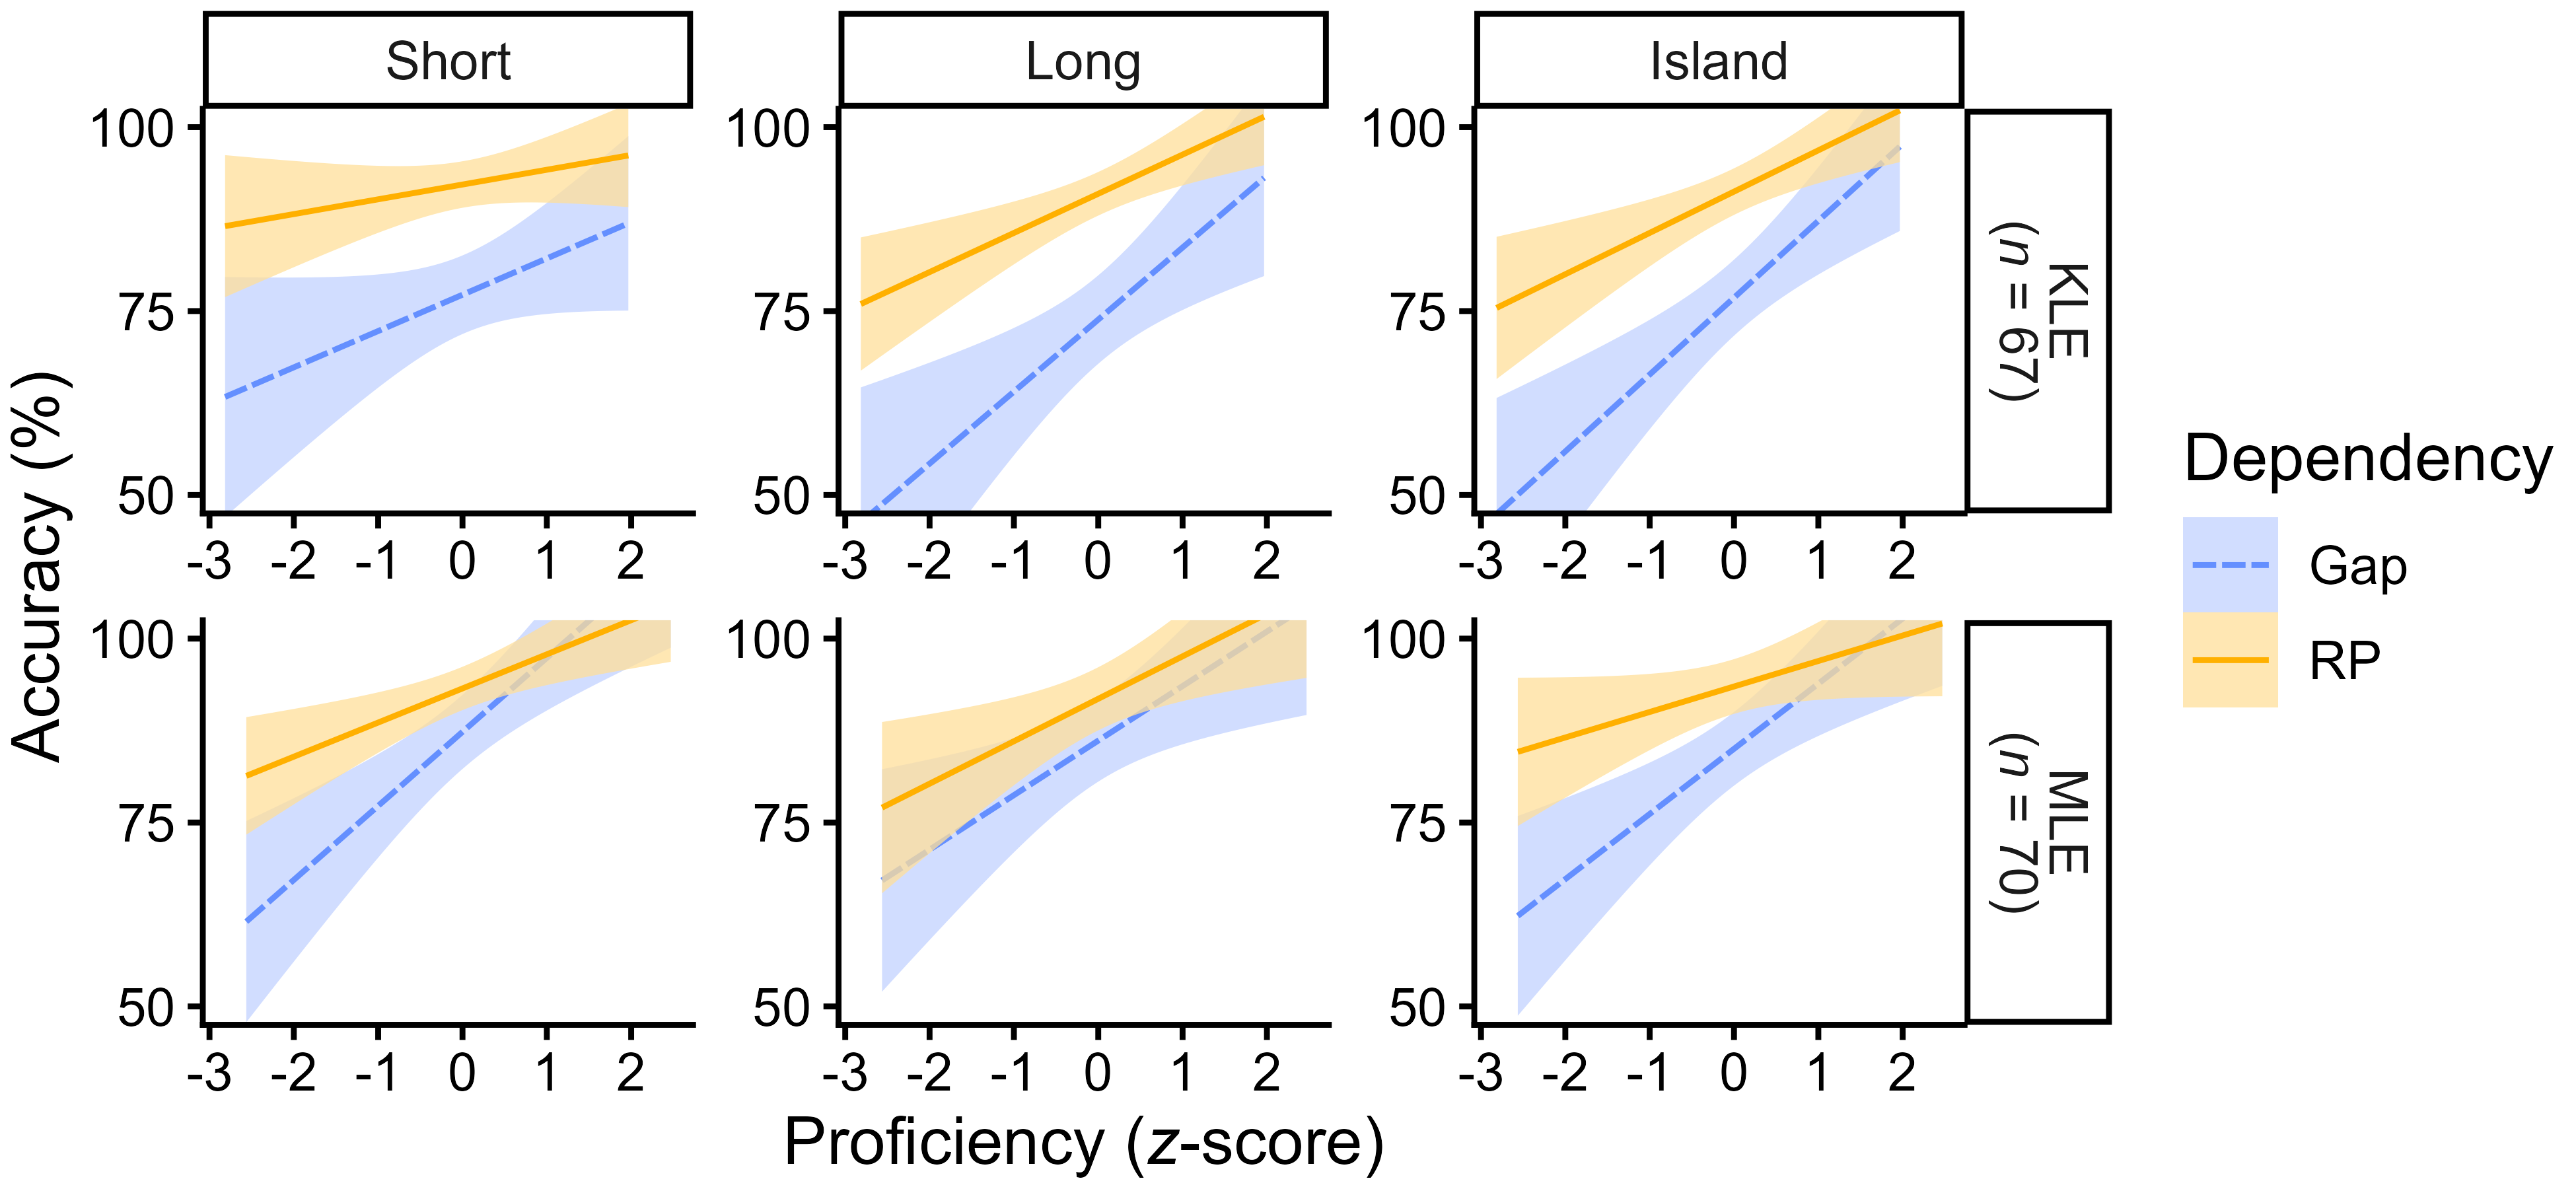
\includegraphics{../analysis/plots/orc_spr_accuracy_proficiency.png}
% \textit{Note}. Shading indicates 95\% $CI$s.
% \vspace{-12pt}
% \end{figure}

% SRC Figure
% \begin{figure}
% \caption{Relationship between L2 proficiency and comprehension-question accuracy in the SRC self-paced reading task} \label{fig:app-src-spr-accuracy-proficiency}
% \raggedright\setstretch{1}
% 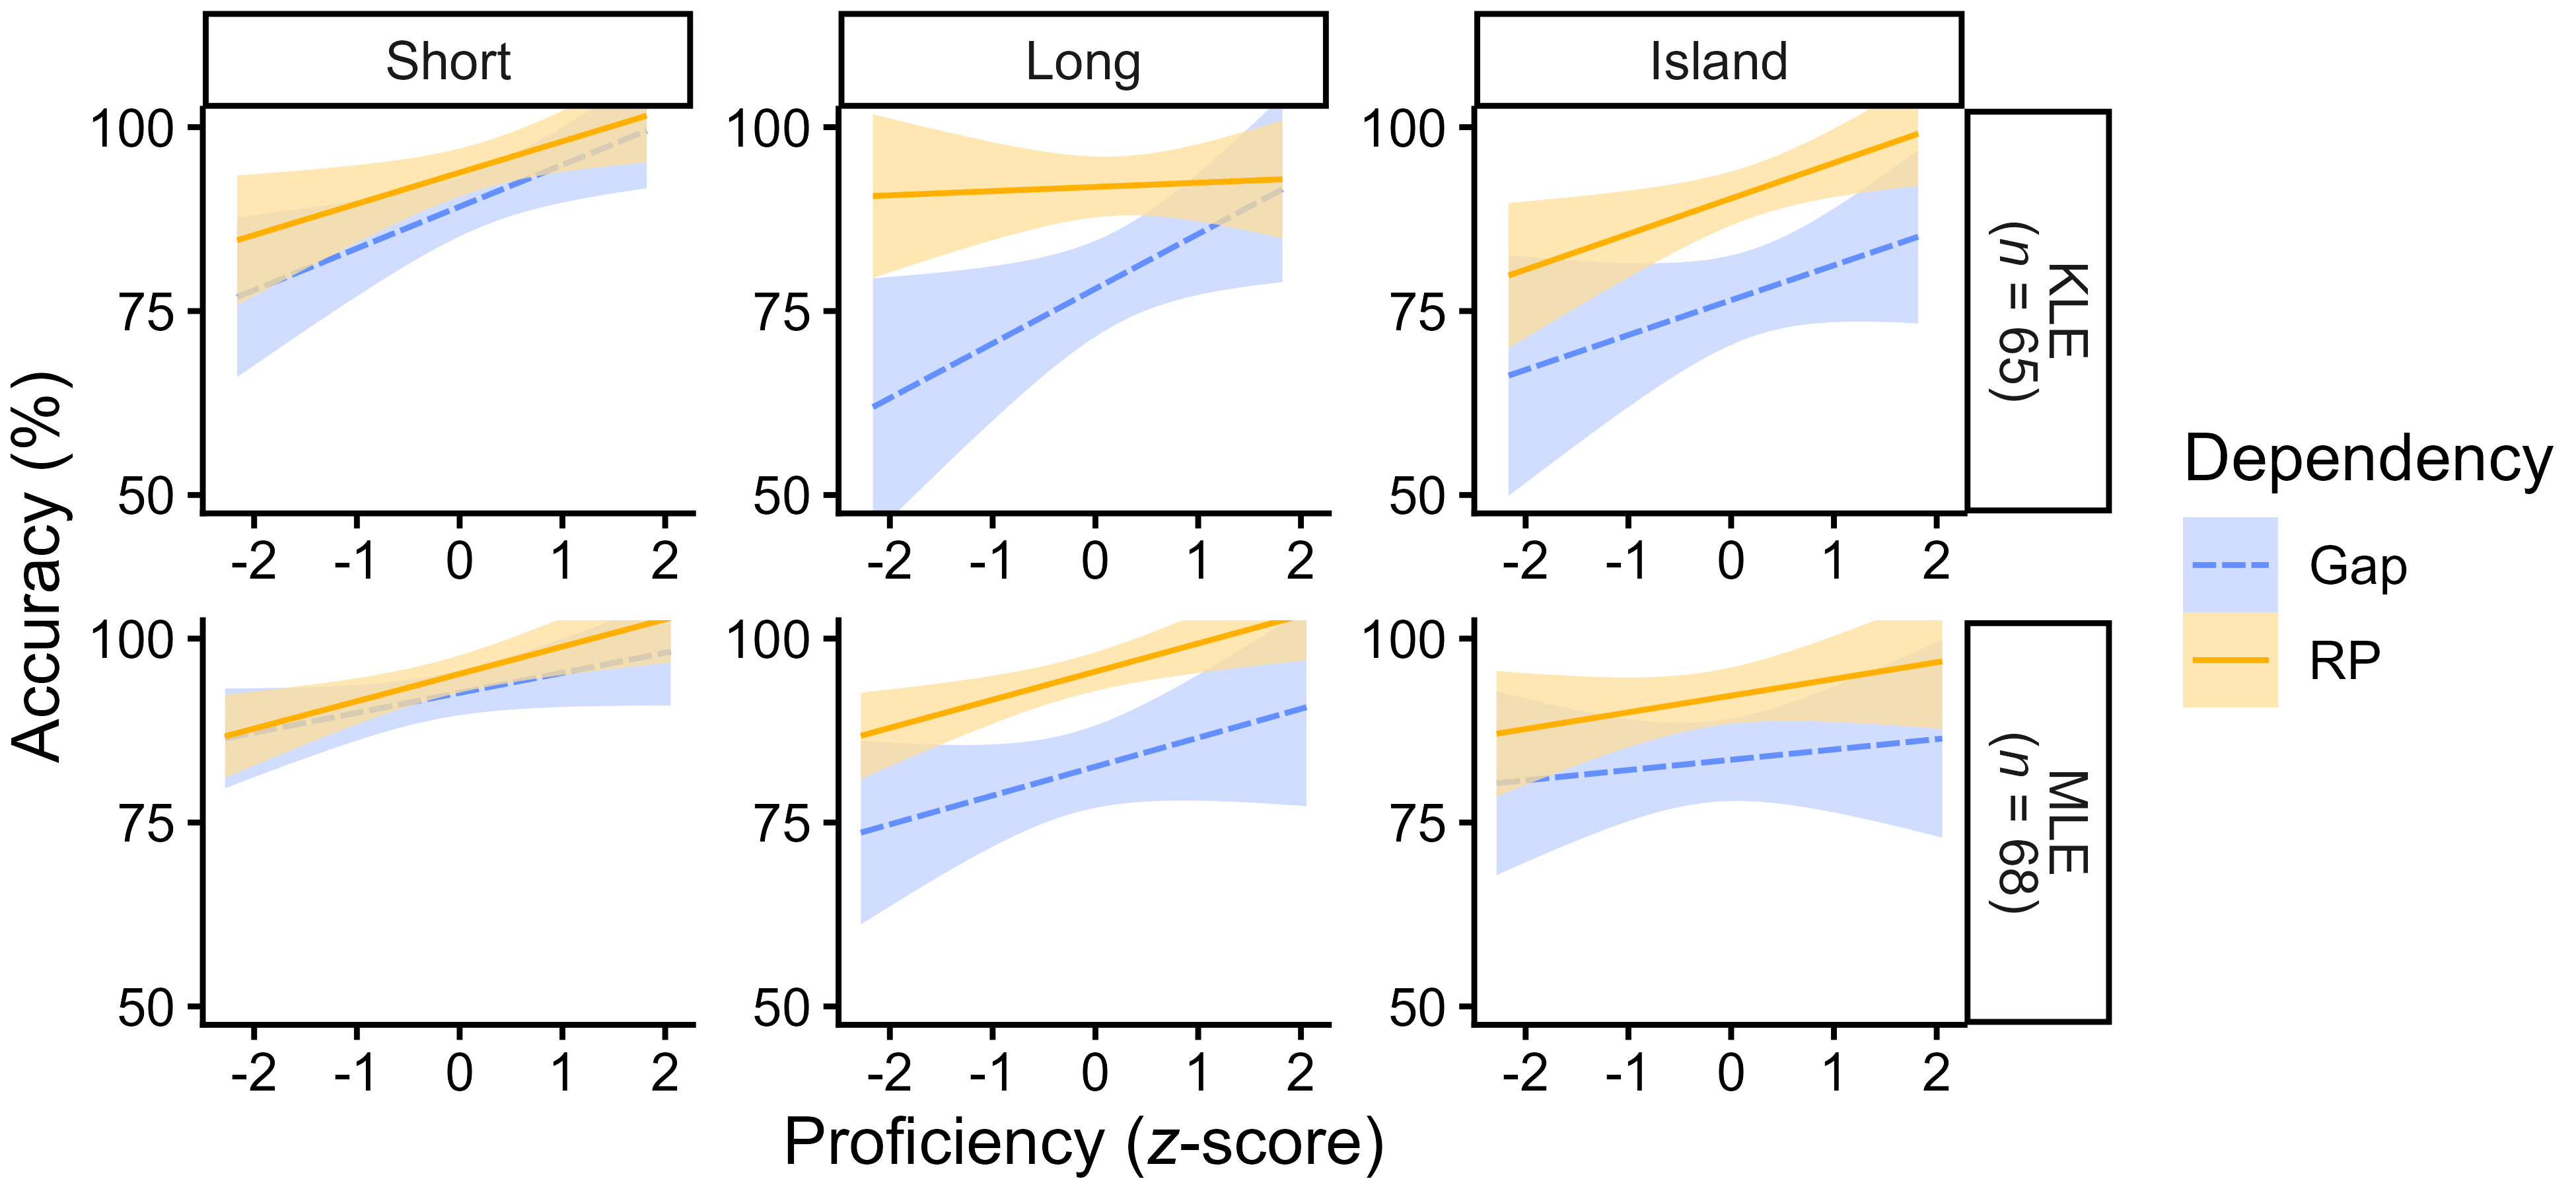
\includegraphics{../analysis/plots/src_spr_accuracy_proficiency.png}
% \textit{Note}. Shading indicates 95\% $CI$s.
% \vspace{-12pt}
% \end{figure}

% ORC Model
\begin{table}
\caption{Summary of mixed-effects logistic regression model for L2 proficiency effects on comprehension-question accuracy in the ORC self-paced reading task}\label{tab:app-orc-spr-accuracy-proficiency-model}
\raggedright\setstretch{1}
\begin{tabularx}{\textwidth}{lrYYY}\toprule
Parameter & Estimate~($\hat{\beta}$) & \textit{SE} & $z$ & $p$ \\\midrule
\csvreader[late after line=\\,late after last line=\\\bottomrule]
{../analysis/tables/orc_spr_accuracy_proficiency_model.csv}{}{\csvcoli & \csvcolii & \csvcoliii & \csvcoliv & \csvcolv}
\end{tabularx}
\textit{Note}. Model formula: Model formula: Accuracy \~{} Dependency * Environment * Group * Proficiency + (1 + Dependency + Environment | Participant) + (1 + Dependency + Environment + Group | Item); reference level: Gap + Short + KLE; estimate unit: logit; intercept: grand mean.
\end{table}

% ORC Posthoc
\begin{table}
\caption{Post-hoc tests for L2 proficiency effects on comprehension-question accuracy in the ORC self-paced reading task}\label{tab:app-orc-spr-accuracy-proficiency-posthoc}
\raggedright\setstretch{1}
\begin{tabularx}{\textwidth}{lXXYYYY}\toprule
Group & Environment & Contrast & Estimate~($\hat{\beta}$) & \textit{SE} & $z$ & $p$ \\\midrule
\csvreader[late after line=\\,late after last line=\\\bottomrule]
{../analysis/tables/orc_spr_accuracy_proficiency_posthoc.csv}{}{\csvcoli & \csvcolii & \csvcoliii & \csvcoliv & \csvcolv & \csvcolvi & \csvcolvii}
\end{tabularx}
\textit{Note}. Adjustment to $p$-values done via multiple $t$ method for 6 tests.
\vspace{-12pt}
\end{table}

% SRC Model
\begin{table}
\caption{Summary of mixed-effects logistic regression model for L2 proficiency effects on comprehension-question accuracy in the SRC self-paced reading task}\label{tab:app-src-spr-accuracy-proficiency-model}
\raggedright\setstretch{1}
\begin{tabularx}{\textwidth}{lrYYY}\toprule
Parameter & Estimate~($\hat{\beta}$) & \textit{SE} & $z$ & $p$ \\\midrule
\csvreader[late after line=\\,late after last line=\\\bottomrule]
{../analysis/tables/src_spr_accuracy_proficiency_model.csv}{}{\csvcoli & \csvcolii & \csvcoliii & \csvcoliv & \csvcolv}
\end{tabularx}
\textit{Note}. Model formula: Model formula: Accuracy \~{} Dependency * Environment * Group * Proficiency + (1 + Dependency | Participant) + (1 + Dependency + Group | Item); reference level: Gap + Short + KLE; estimate unit: logit; intercept: grand mean.
\end{table}

% SRC Posthoc
\begin{table}
\caption{Post-hoc tests for L2 proficiency effects on comprehension-question accuracy in the SRC self-paced reading task}\label{tab:app-src-spr-accuracy-proficiency-posthoc}
\raggedright\setstretch{1}
\begin{tabularx}{\textwidth}{lXXYYYY}\toprule
Group & Environment & Contrast & Estimate~($\hat{\beta}$) & \textit{SE} & $z$ & $p$ \\\midrule
\csvreader[late after line=\\,late after last line=\\\bottomrule]
{../analysis/tables/src_spr_accuracy_proficiency_posthoc.csv}{}{\csvcoli & \csvcolii & \csvcoliii & \csvcoliv & \csvcolv & \csvcolvi & \csvcolvii}
\end{tabularx}
\textit{Note}. Adjustment to $p$-values done via multiple $t$ method for 6 tests.
\end{table}

%========================================================%
\section{Comprehension-question RTs}\label{app-spr-qrt}
%========================================================%

% ORC Raw RT Table
% \DTLloaddb{dt-spr-question-rt}{../analysis/tables/spr_question_rt.csv}
% \ExplSyntaxOn
% \tl_clear:N \tblrbody
% \tl_build_begin:N \tblrbody
% \DTLforeach[\equal{\study}{ORC}]{dt-spr-question-rt}{\study=study,\coli=Group,\colii=Dependency,\coliii=Environment,\coliv=Mean,\colv=$CI$}{\tl_build_put_right:Ne \tblrbody {\exp_not:V \coli & \exp_not:V \colii & \exp_not:V \coliii & \exp_not:V \coliv & \exp_not:V \colv\\}}
% \tl_build_end:N \tblrbody
% \ExplSyntaxOff
% \begin{longtblr}[caption={Mean raw RTs for comprehension questions in the ORC self-paced reading task}, label={tblr:app-orc-spr-question-rt}, expand=\tblrbody]{colspec={lXXX[r]X[r]}}\toprule
% Group~~~~~ & Dependency & Environment & Mean & 95\%~\textit{CI}\\\midrule
% \tblrbody\bottomrule
% \end{longtblr}
% \vspace{-12pt}

% SRC Raw RT Table
% \ExplSyntaxOn
% \tl_clear:N \tblrbody
% \tl_build_begin:N \tblrbody
% \DTLforeach[\equal{\study}{SRC}]{dt-spr-question-rt}{\study=study,\coli=Group,\colii=Dependency,\coliii=Environment,\coliv=Mean,\colv=$CI$}{\tl_build_put_right:Ne \tblrbody {\exp_not:V \coli & \exp_not:V \colii & \exp_not:V \coliii & \exp_not:V \coliv & \exp_not:V \colv\\}}
% \tl_build_end:N \tblrbody
% \ExplSyntaxOff
% \begin{longtblr}[caption={Mean raw RTs for comprehension questions in the SRC self-paced reading task}, label={tblr:src-spr-question-rt}, expand=\tblrbody]{colspec={lXXX[r]X[r]}}\toprule
% Group~~~~~ & Dependency & Environment & Mean & 95\%~\textit{CI}\\\midrule
% \tblrbody\bottomrule
% \end{longtblr}
% \vspace{-12pt}

% ORC Raw RT Figure
\begin{figure}
\caption{Mean raw RTs for comprehension questions in the ORC self-paced reading task} \label{fig:app-orc-spr-question-rt}
\raggedright\setstretch{1}
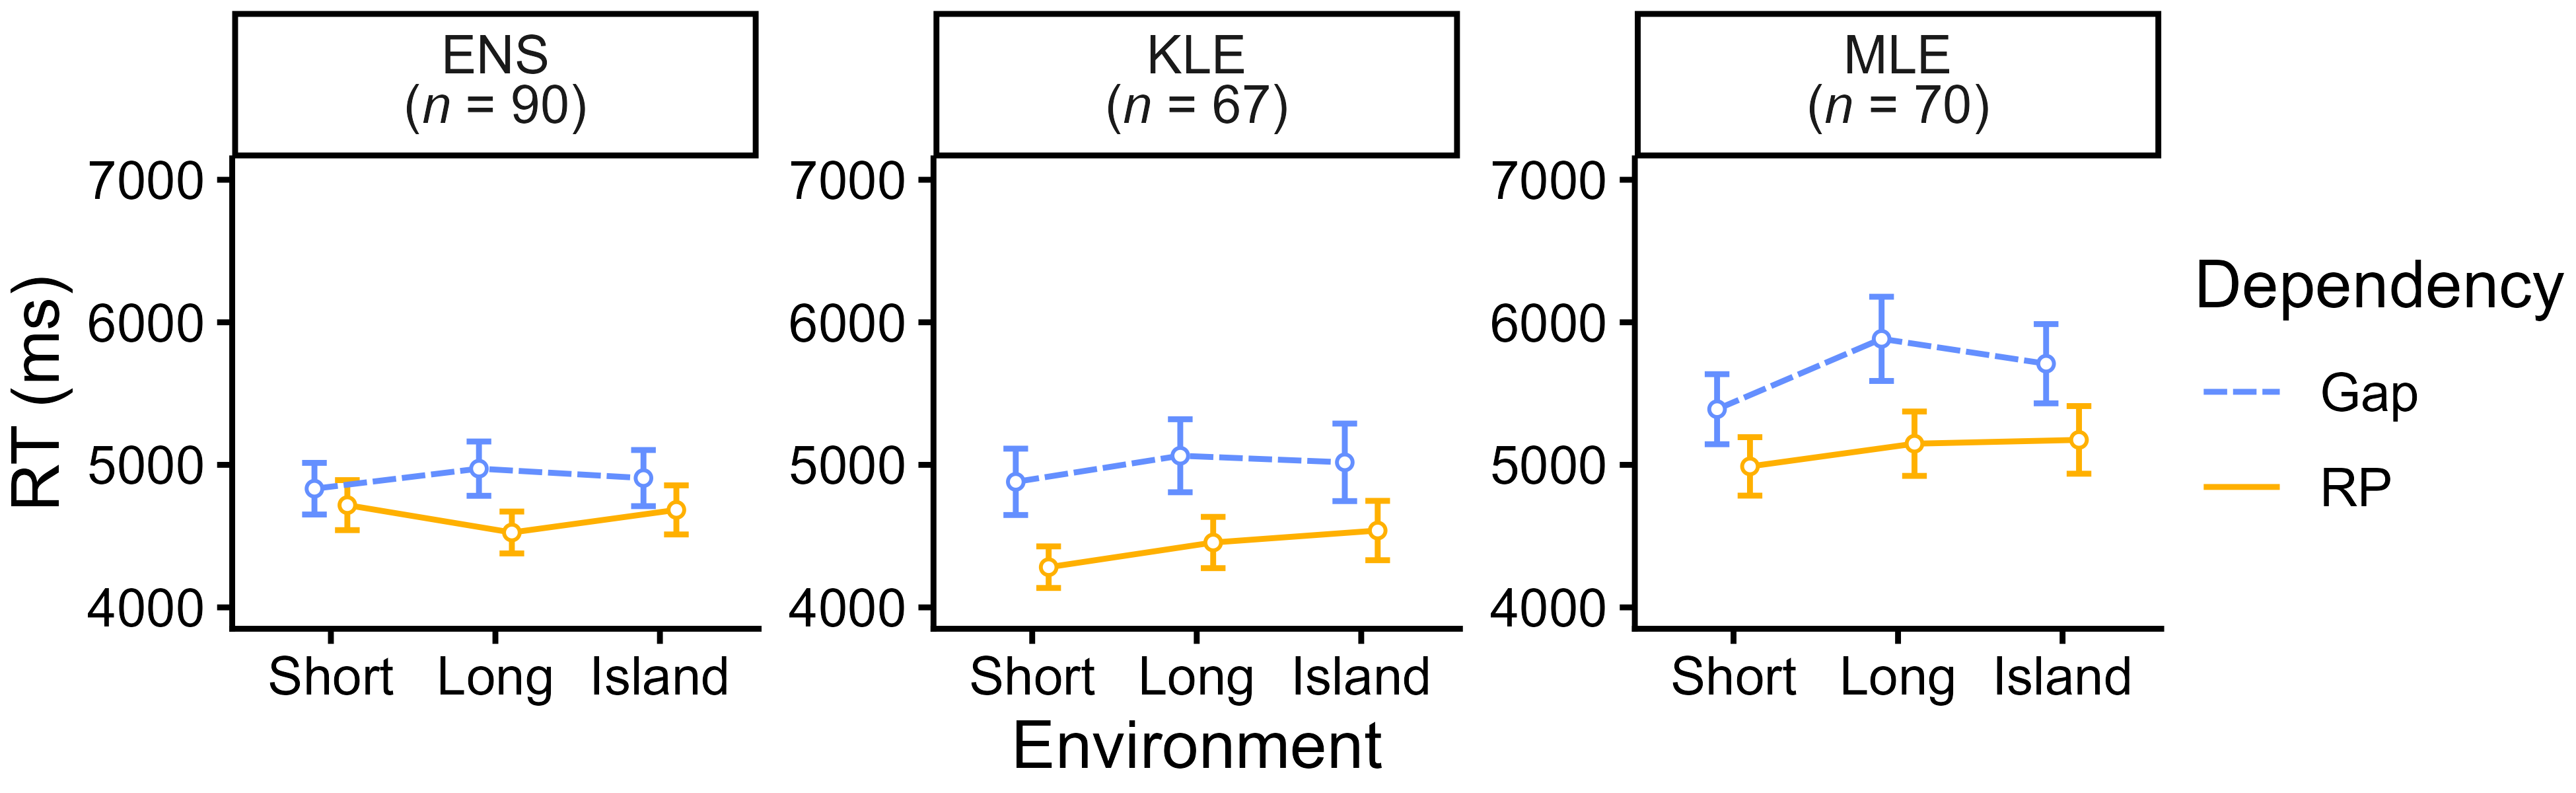
\includegraphics[width=\textwidth]{../analysis/plots/orc_spr_question_rt_overall.png}
\textit{Note}. Error bars are 95\% \textit{CI}s.
\vspace{-12pt}
\end{figure}

% SRC Raw RT Figure
\begin{figure}
\caption{Mean raw RTs for comprehension questions in the SRC self-paced reading task} \label{fig:app-src-spr-question-rt}
\raggedright\setstretch{1}
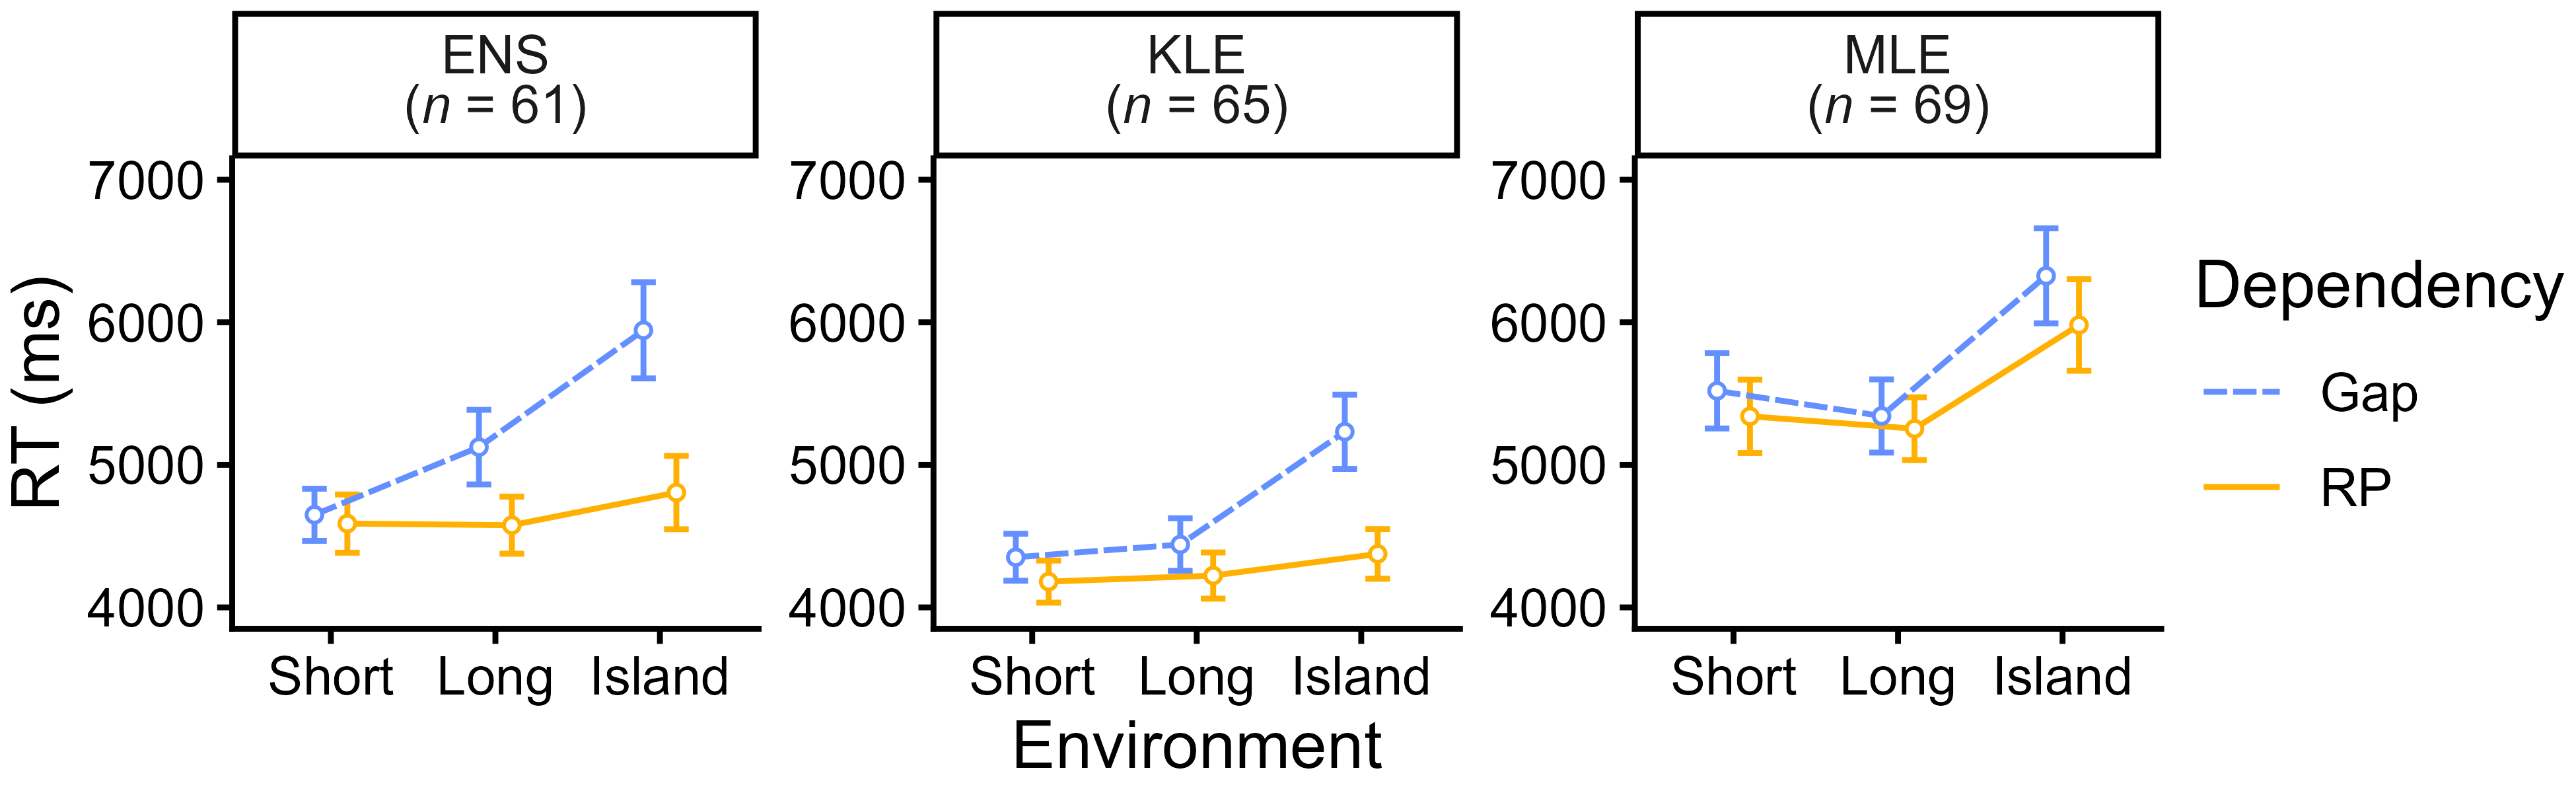
\includegraphics[width=\textwidth]{../analysis/plots/src_spr_question_rt_overall.png}
\textit{Note}. Error bars are 95\% \textit{CI}s.
\vspace{-12pt}
\end{figure}

% ORC Log RT Table
% \DTLloaddb{dt-spr-question-logrt}{../analysis/tables/spr_question_logrt.csv}
% \ExplSyntaxOn
% \tl_clear:N \tblrbody
% \tl_build_begin:N \tblrbody
% \DTLforeach[\equal{\study}{ORC}]{dt-spr-question-logrt}{\study=study,\coli=Group,\colii=Dependency,\coliii=Environment,\coliv=Mean,\colv=$CI$}{\tl_build_put_right:Ne \tblrbody {\exp_not:V \coli & \exp_not:V \colii & \exp_not:V \coliii & \exp_not:V \coliv & \exp_not:V \colv\\}}
% \tl_build_end:N \tblrbody
% \ExplSyntaxOff
% \begin{longtblr}[caption={Mean log RTs for comprehension questions in the ORC self-paced reading task}, label={tblr:app-orc-spr-question-logrt}, expand=\tblrbody]{colspec={lXXX[r]X[r]}}\toprule
% Group~~~~~ & Dependency & Environment & Mean & 95\%~\textit{CI}\\\midrule
% \tblrbody\bottomrule
% \end{longtblr}
% \vspace{-12pt}

% SRC Log RT Table
% \ExplSyntaxOn
% \tl_clear:N \tblrbody
% \tl_build_begin:N \tblrbody
% \DTLforeach[\equal{\study}{SRC}]{dt-spr-question-logrt}{\study=study,\coli=Group,\colii=Dependency,\coliii=Environment,\coliv=Mean,\colv=$CI$}{\tl_build_put_right:Ne \tblrbody {\exp_not:V \coli & \exp_not:V \colii & \exp_not:V \coliii & \exp_not:V \coliv & \exp_not:V \colv\\}}
% \tl_build_end:N \tblrbody
% \ExplSyntaxOff
% \begin{longtblr}[caption={Mean log RTs for comprehension questions in the SRC self-paced reading task}, label={tblr:src-spr-question-logrt}, expand=\tblrbody]{colspec={lXXX[r]X[r]}}\toprule
% Group~~~~~ & Dependency & Environment & Mean & 95\%~\textit{CI}\\\midrule
% \tblrbody\bottomrule
% \end{longtblr}
% \vspace{-12pt}

% ORC Log RT Figure
% \begin{figure}
% \caption{Mean comprehension-question log RTs in the ORC self-paced reading task} \label{fig:app-orc-spr-question-logrt}
% \raggedright\setstretch{1}
% 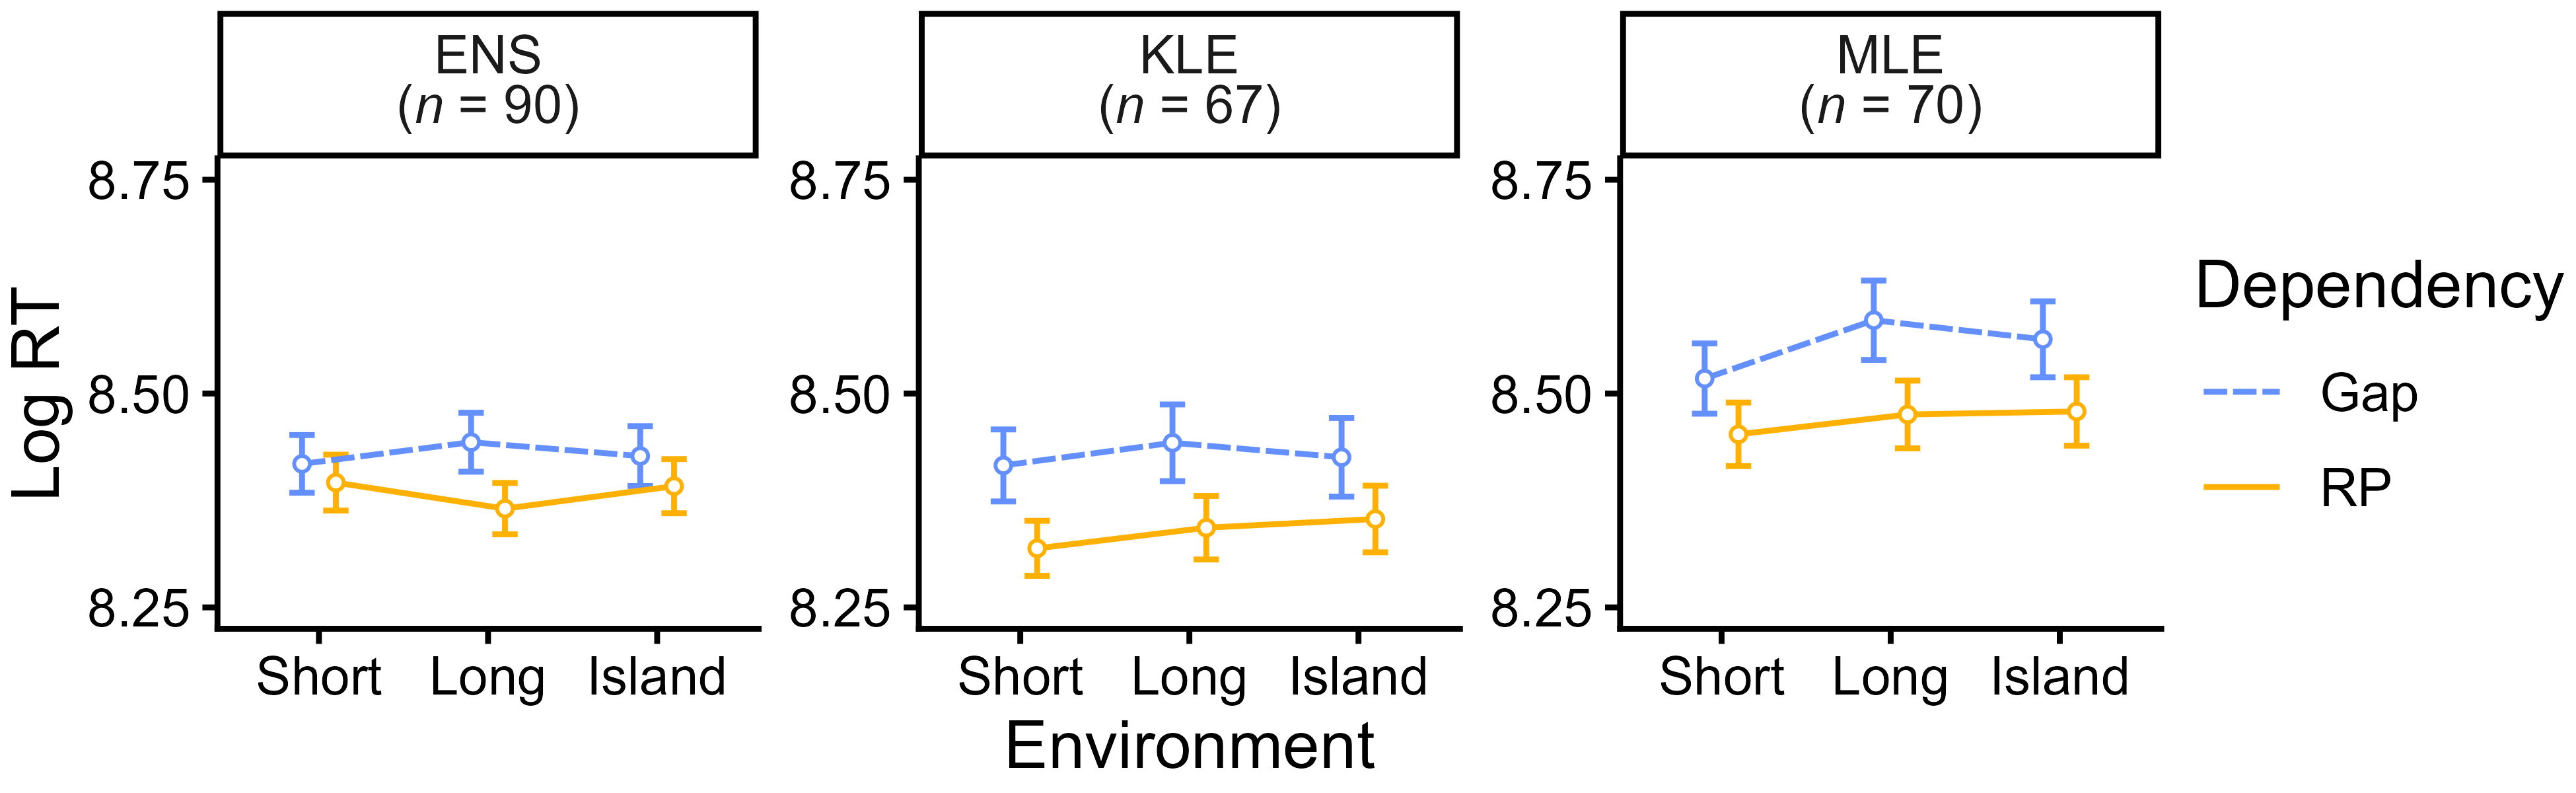
\includegraphics[width=\textwidth]{../analysis/plots/orc_spr_question_logrt_overall.png}
% \textit{Note}. Error bars are 95\% \textit{CI}s.
% \vspace{-12pt}
% \end{figure}

% SRC Log RT Figure
% \begin{figure}
% \caption{Mean comprehension-question log RTs in the SRC self-paced reading task} \label{fig:app-src-spr-question-logrt}
% \raggedright\setstretch{1}
% 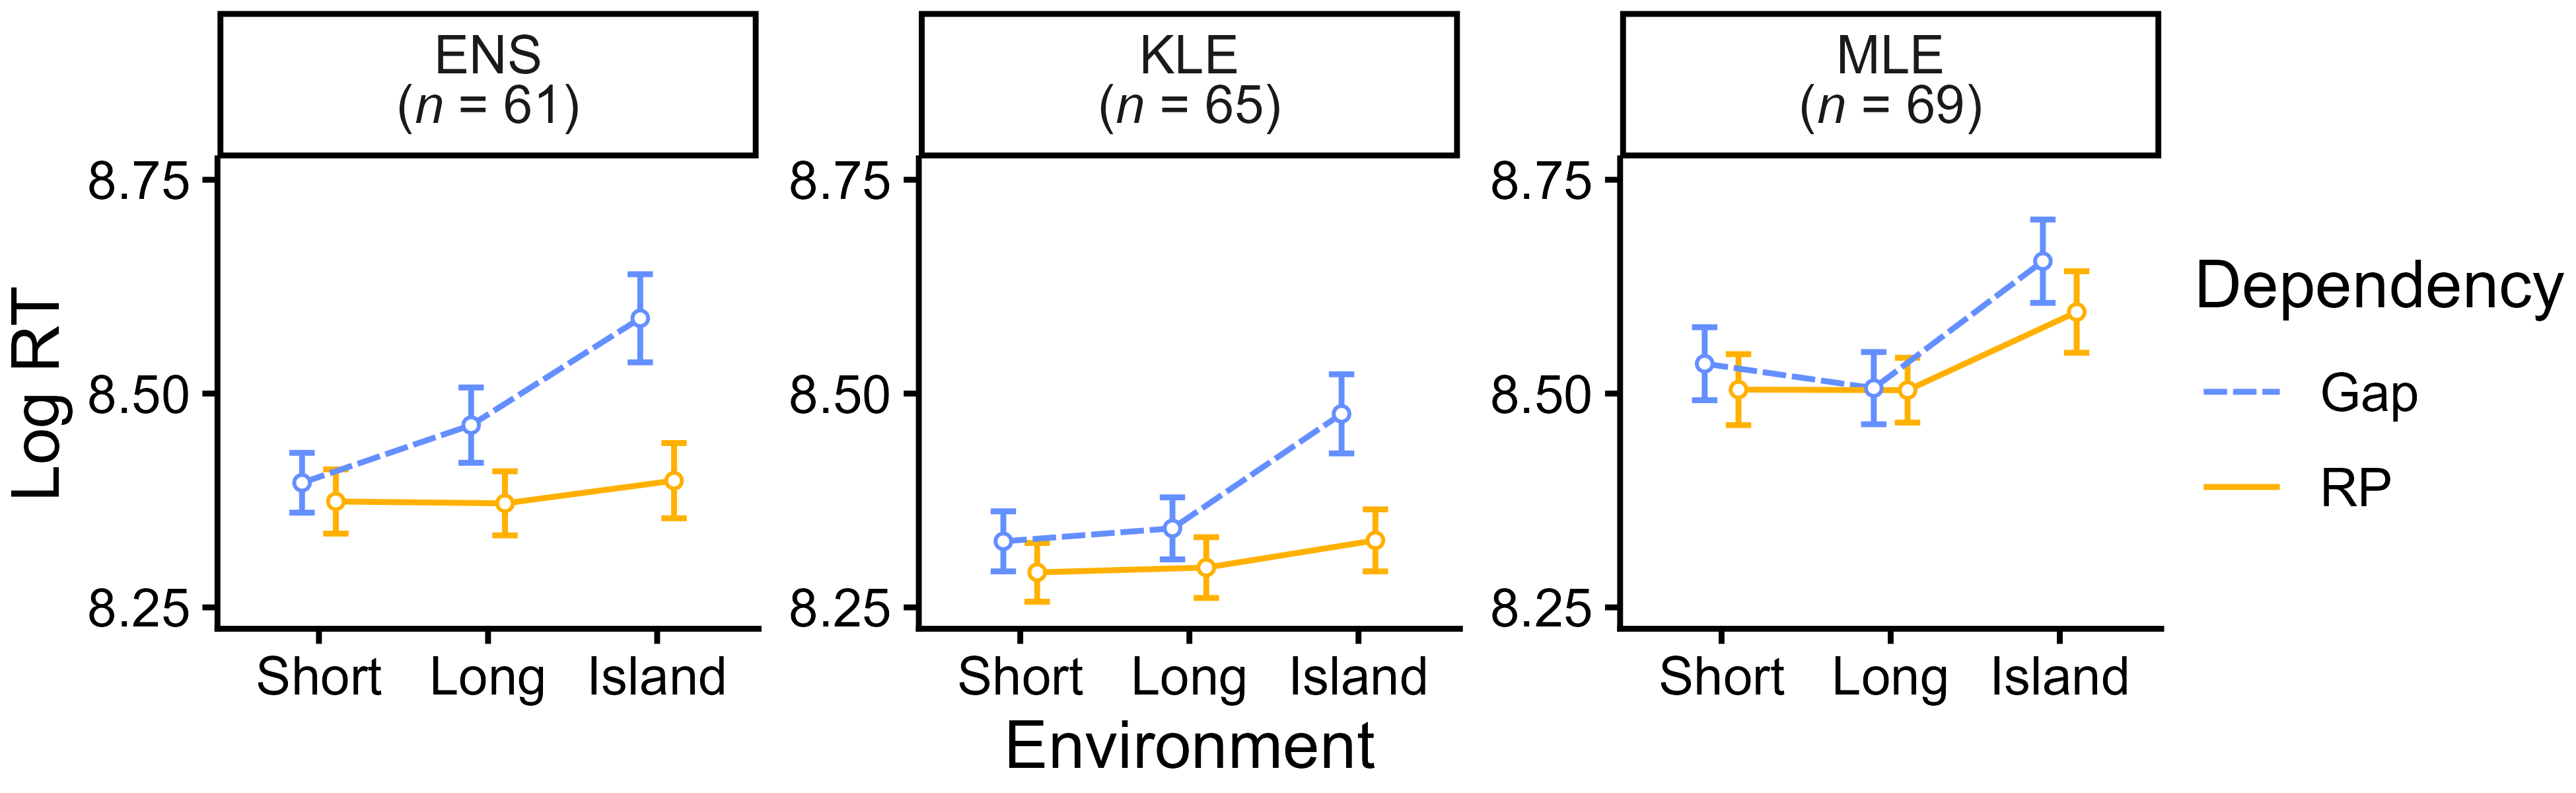
\includegraphics[width=\textwidth]{../analysis/plots/src_spr_question_logrt_overall.png}
% \textit{Note}. Error bars are 95\% \textit{CI}s.
% \vspace{-12pt}
% \end{figure}

% ORC Model
\DTLloaddb{dt-orc-spr-question-logrt-model}{../analysis/tables/orc_spr_question_logrt_model.csv}
\ExplSyntaxOn
\tl_clear:N \tblrbody
\tl_build_begin:N \tblrbody
\DTLforeach{dt-orc-spr-question-logrt-model}{\coli=Parameter,\colii=Estimate,\coliii=$SE$,\coliv=$t$,\colv=$p$}{\tl_build_put_right:Ne \tblrbody {\exp_not:V \coli & \exp_not:V \colii & \exp_not:V \coliii & \exp_not:V \coliv & \exp_not:V \colv\\}}
\tl_build_end:N \tblrbody
\ExplSyntaxOff
\begin{longtblr}[caption={Summary of linear mixed-effects model on comprehension-question log RTs in the ORC self-paced reading task}, label={tblr:app-orc-spr-question-logrt-model}, expand=\tblrbody, remark{Note}={Model formula: Model formula: Log RT \~{} Dependency * Environment * Group + (1 + Dependency + Environment | Participant) + (1 + Dependency + Environment + Group | Item); reference level: Gap + Short + ENS; estimate unit: log RT; intercept: grand mean.}]{colspec={lX[r]X[r]X[r]X[r]}}\toprule
Parameter & Estimate~($\hat{\beta}$) & \textit{SE} & $t$ & $p$\\\midrule
\tblrbody\bottomrule
\end{longtblr}
\vspace{-12pt}

% ORC Posthoc
\DTLloaddb{dt-orc-spr-question-logrt-posthoc}{../analysis/tables/orc_spr_question_logrt_posthoc.csv}
\ExplSyntaxOn
\tl_clear:N \tblrbody
\tl_build_begin:N \tblrbody
\DTLforeach{dt-orc-spr-question-logrt-posthoc}{\coli=Group,\colii=Environment,\coliii=Contrast,\coliv=Estimate,\colv=$SE$,\colvi=$z$,\colvii=$p$}{\tl_build_put_right:Ne \tblrbody {\exp_not:V \coli & \exp_not:V \colii & \exp_not:V \coliii & \exp_not:V \coliv & \exp_not:V \colv & \exp_not:V \colvi & \exp_not:V \colvii\\}}
\tl_build_end:N \tblrbody
\ExplSyntaxOff
\begin{longtblr}[caption={Post-hoc tests for comprehension-question log RTs in the ORC self-paced reading task}, label={tblr:app-orc-spr-question-logrt-posthoc}, expand=\tblrbody, remark{Note}={Adjustment to $p$-values done via multiple $t$ method for 9 tests.}]{colspec={XXXX[r]X[r]X[r]X[r]}}\toprule
Group & Environment & Contrast & Estimate~($\hat{\beta}$) & \textit{SE} & $z$ & $p$\\\midrule
\tblrbody\bottomrule
\end{longtblr}
\vspace{-12pt}

% SRC Model
\DTLloaddb{dt-src-spr-question-logrt-model}{../analysis/tables/src_spr_question_logrt_model.csv}
\ExplSyntaxOn
\tl_clear:N \tblrbody
\tl_build_begin:N \tblrbody
\DTLforeach{dt-src-spr-question-logrt-model}{\coli=Parameter,\colii=Estimate,\coliii=$SE$,\coliv=$t$,\colv=$p$}{\tl_build_put_right:Ne \tblrbody {\exp_not:V \coli & \exp_not:V \colii & \exp_not:V \coliii & \exp_not:V \coliv & \exp_not:V \colv\\}}
\tl_build_end:N \tblrbody
\ExplSyntaxOff
\begin{longtblr}[caption={Summary of linear mixed-effects model on comprehension-question log RTs in the SRC self-paced reading task}, label={tblr:app-src-spr-question-logrt-model}, expand=\tblrbody, remark{Note}={Model formula: Model formula: Log RT \~{} Dependency * Environment * Group + (1 + Dependency + Environment | Participant) + (1 + Dependency + Environment + Group | Item); reference level: Gap + Short + ENS; estimate unit: log RT; intercept: grand mean.}]{colspec={lX[r]X[r]X[r]X[r]}}\toprule
Parameter & Estimate~($\hat{\beta}$) & \textit{SE} & $t$ & $p$\\\midrule
\tblrbody\bottomrule
\end{longtblr}
\vspace{-12pt}

% SRC Posthoc
\DTLloaddb{dt-src-spr-question-logrt-posthoc}{../analysis/tables/src_spr_question_logrt_posthoc.csv}
\ExplSyntaxOn
\tl_clear:N \tblrbody
\tl_build_begin:N \tblrbody
\DTLforeach{dt-src-spr-question-logrt-posthoc}{\coli=Group,\colii=Environment,\coliii=Contrast,\coliv=Estimate,\colv=$SE$,\colvi=$z$,\colvii=$p$}{\tl_build_put_right:Ne \tblrbody {\exp_not:V \coli & \exp_not:V \colii & \exp_not:V \coliii & \exp_not:V \coliv & \exp_not:V \colv & \exp_not:V \colvi & \exp_not:V \colvii\\}}
\tl_build_end:N \tblrbody
\ExplSyntaxOff
\begin{longtblr}[caption={Post-hoc tests for comprehension-question log RTs in the SRC self-paced reading task}, label={tblr:src-spr-question-logrt-posthoc}, expand=\tblrbody, remark{Note}={Adjustment to $p$-values done via multiple $t$ method for 9 tests.}]{colspec={XXXX[r]X[r]X[r]X[r]}}\toprule
Group & Environment & Contrast & Estimate~($\hat{\beta}$) & \textit{SE} & $z$ & $p$\\\midrule
\tblrbody\bottomrule
\end{longtblr}
\vspace{-12pt}

%========================================================%
\section{L2 proficiency effects for comprehension-question log RTs}\label{app-app-spr-qrt-proficiency}
%========================================================%

% ORC Figure
% \begin{figure}
% \caption{Relationship between L2 proficiency and comprehension-question log RTs in the ORC self-paced reading task} \label{fig:app-orc-spr-question-logrt-proficiency}
% \raggedright\setstretch{1}
% 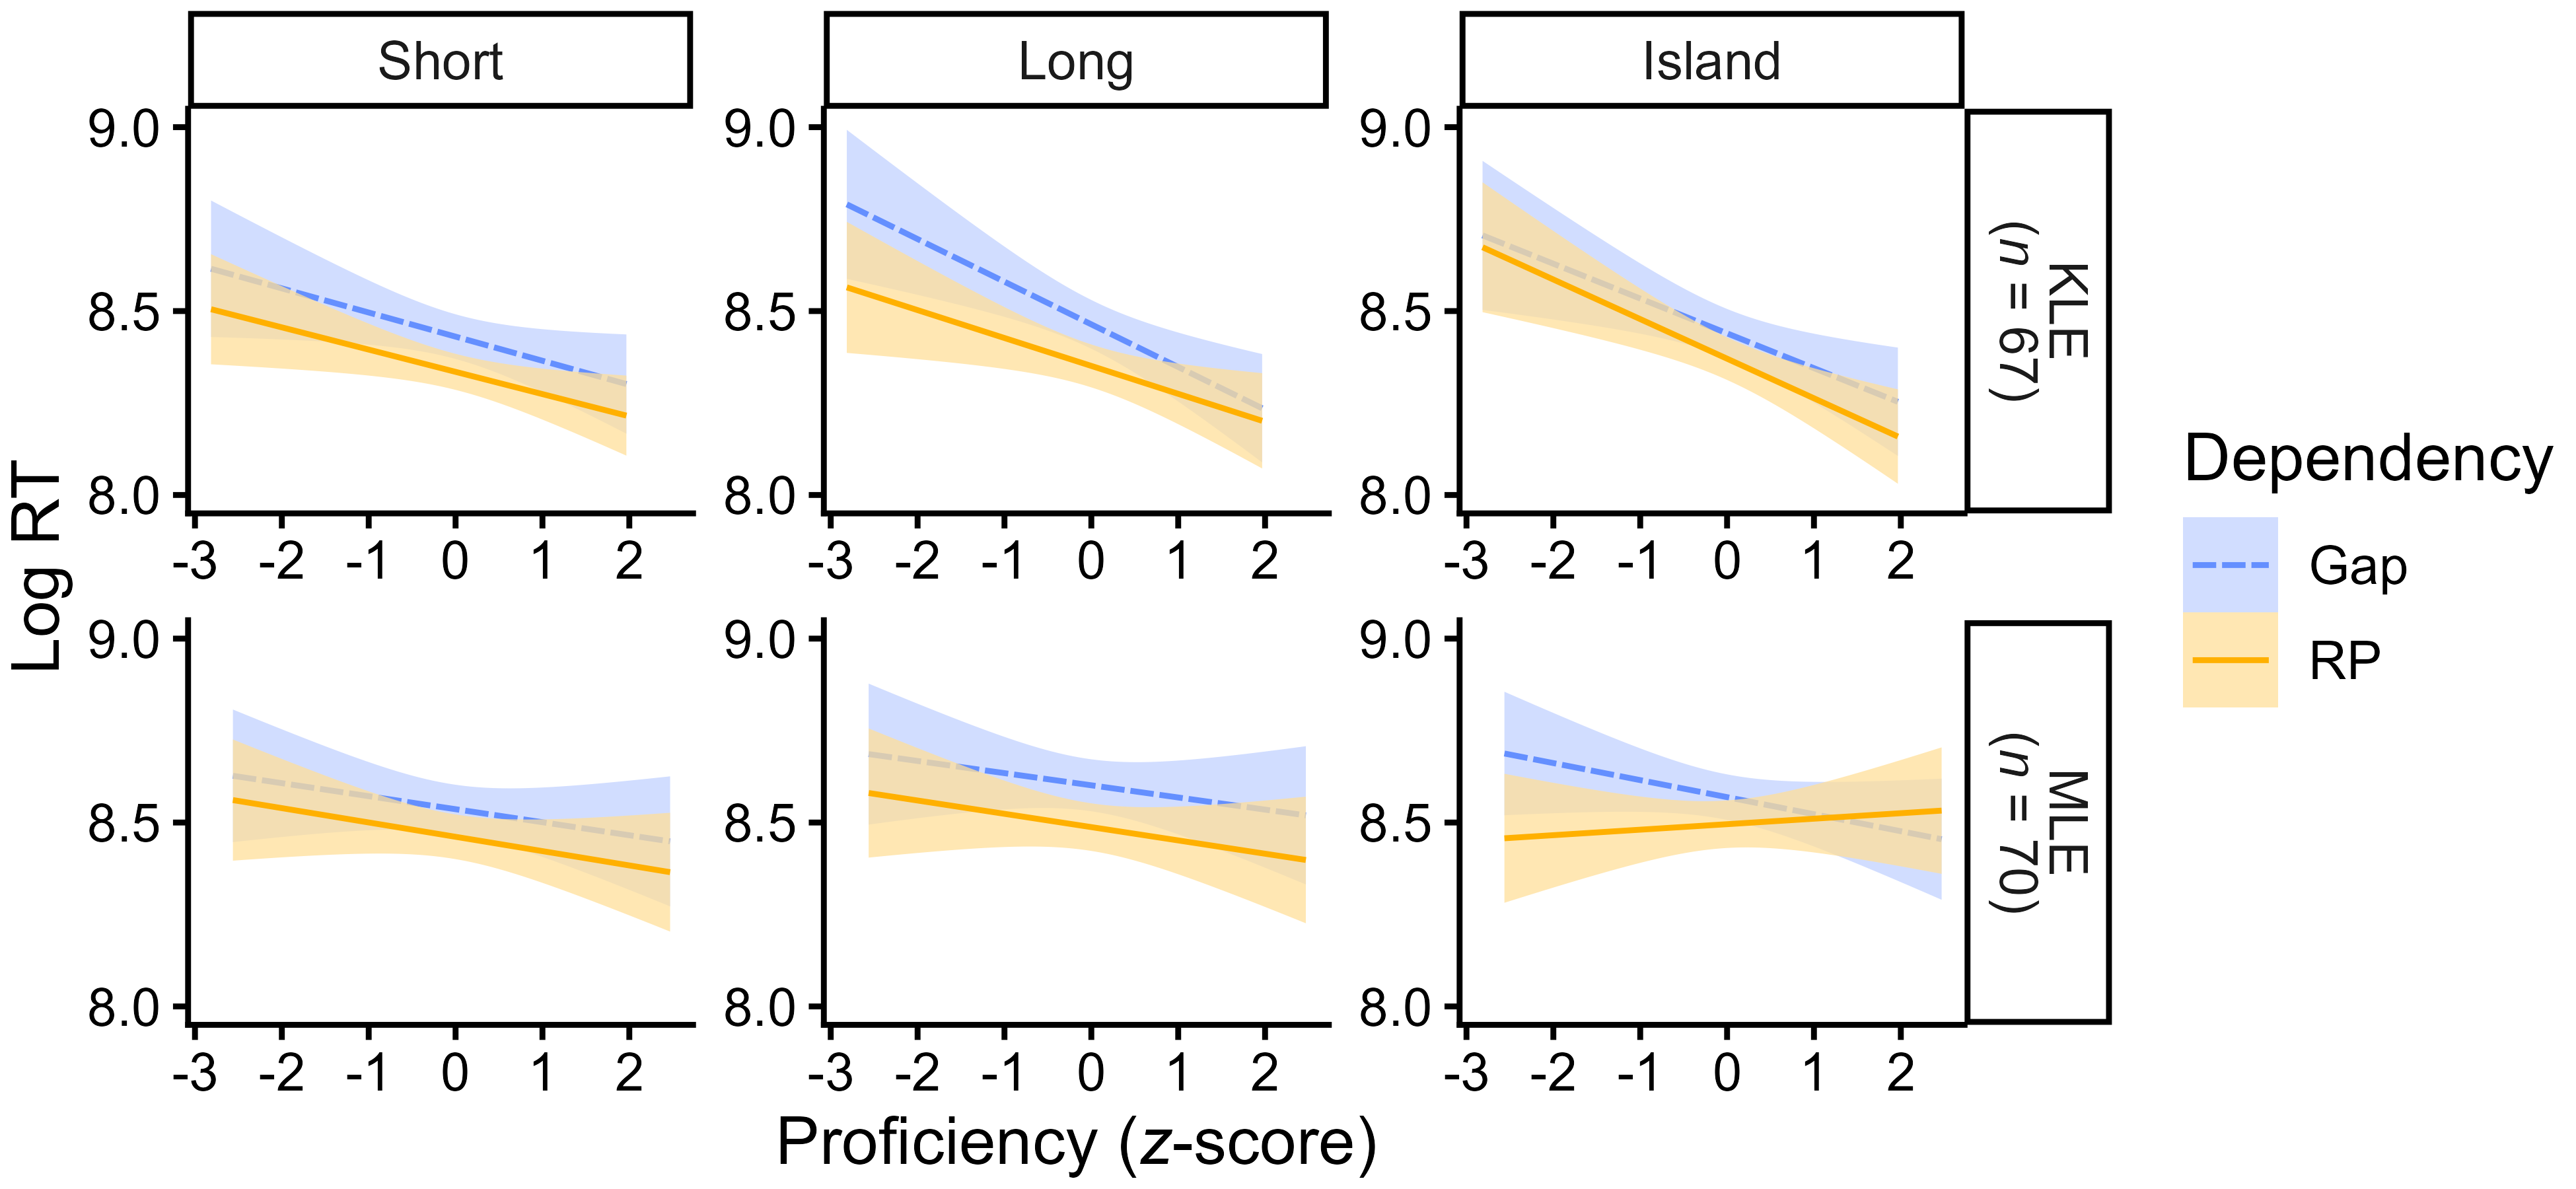
\includegraphics[width=\textwidth]{../analysis/plots/orc_spr_question_logrt_proficiency.png}
% \textit{Note}. Shading indicates 95\% \textit{CI}s.
% \vspace{-12pt}
% \end{figure}

% SRC Figure
% \begin{figure}
% \caption{Relationship between L2 proficiency and comprehension-question log RTs in the SRC self-paced reading task} \label{fig:app-src-spr-question-logrt-proficiency}
% \raggedright\setstretch{1}
% 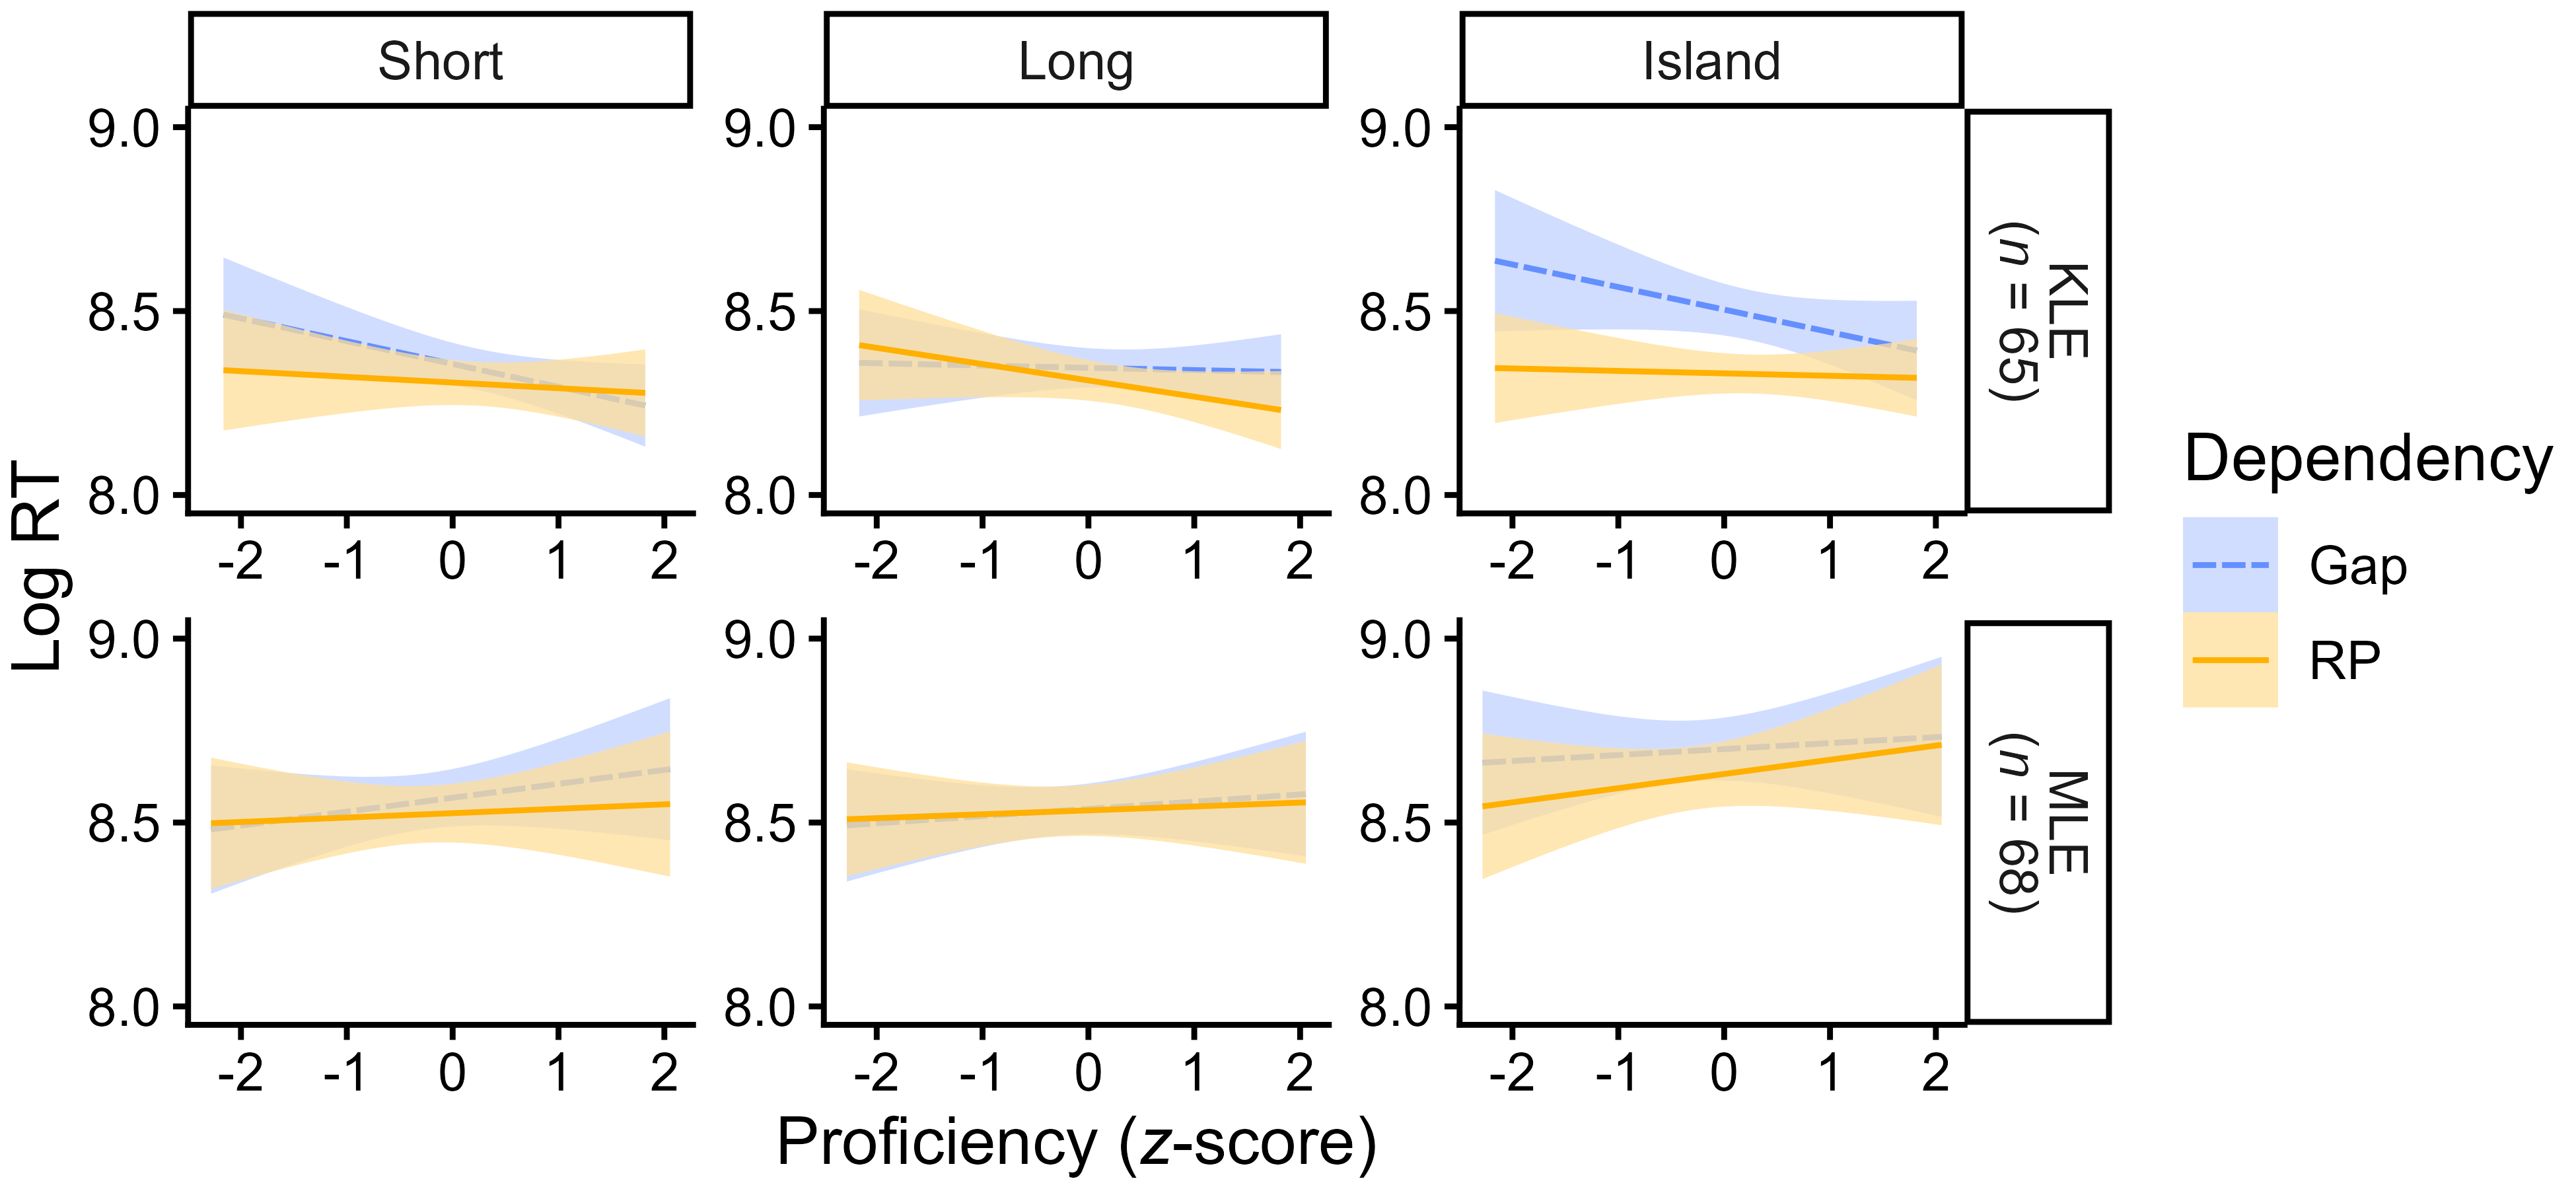
\includegraphics[width=\textwidth]{../analysis/plots/src_spr_question_logrt_proficiency.png}
% \textit{Note}. Shading indicates 95\% \textit{CI}s.
% \vspace{-12pt}
% \end{figure}

% ORC Model
\DTLloaddb{dt-orc-spr-question-logrt-proficiency-model}{../analysis/tables/orc_spr_question_logrt_proficiency_model.csv}
\ExplSyntaxOn
\tl_clear:N \tblrbody
\tl_build_begin:N \tblrbody
\DTLforeach{dt-orc-spr-question-logrt-proficiency-model}{\coli=Parameter,\colii=Estimate,\coliii=$SE$,\coliv=$t$,\colv=$p$}{\tl_build_put_right:Ne \tblrbody {\exp_not:V \coli & \exp_not:V \colii & \exp_not:V \coliii & \exp_not:V \coliv & \exp_not:V \colv\\}}
\tl_build_end:N \tblrbody
\ExplSyntaxOff
\begin{longtblr}[caption={Summary of linear mixed-effects model for L2 proficiency effects on comprehension-question log RTs in the ORC self-paced reading task}, label={tblr:app-orc-spr-question-logrt-proficiency-model}, expand=\tblrbody, remark{Note}={Model formula: Model formula: Log RT \~{} Dependency * Environment * Group * Proficiency + (1 + Dependency + Environment | Participant) + (1 + Dependency + Environment | Item); reference level: Gap + Short + KLE; estimate unit: log RT; intercept: grand mean.}]{colspec={lX[r]X[r]X[r]X[r]}}\toprule
Parameter & Estimate~($\hat{\beta}$) & \textit{SE} & $t$ & $p$\\\midrule
\tblrbody\bottomrule
\end{longtblr}
\vspace{-12pt}

% ORC Posthoc
\DTLloaddb{dt-orc-spr-question-logrt-proficiency-posthoc}{../analysis/tables/orc_spr_question_logrt_proficiency_posthoc.csv}
\ExplSyntaxOn
\tl_clear:N \tblrbody
\tl_build_begin:N \tblrbody
\DTLforeach{dt-orc-spr-question-logrt-proficiency-posthoc}{\coli=Group,\colii=Environment,\coliii=Contrast,\coliv=Estimate,\colv=$SE$,\colvi=$z$,\colvii=$p$}{\tl_build_put_right:Ne \tblrbody {\exp_not:V \coli & \exp_not:V \colii & \exp_not:V \coliii & \exp_not:V \coliv & \exp_not:V \colv & \exp_not:V \colvi & \exp_not:V \colvii\\}}
\tl_build_end:N \tblrbody
\ExplSyntaxOff
\begin{longtblr}[caption={Post-hoc tests for L2 proficiency trend on comprehension-question log RTs in the ORC self-paced reading task}, label={tblr:app-orc-spr-question-logrt-proficiency-posthoc}, expand=\tblrbody, remark{Note}={Adjustment to $p$-values done via multiple $t$ method for 9 tests.}]{colspec={XXXX[r]X[r]X[r]X[r]}}\toprule
Group & Environment & Contrast & Estimate~($\hat{\beta}$) & \textit{SE} & $z$ & $p$\\\midrule
\tblrbody\bottomrule
\end{longtblr}
\vspace{-12pt}

% SRC Model
\DTLloaddb{dt-src-spr-question-logrt-proficiency-model}{../analysis/tables/src_spr_question_logrt_proficiency_model.csv}
\ExplSyntaxOn
\tl_clear:N \tblrbody
\tl_build_begin:N \tblrbody
\DTLforeach{dt-src-spr-question-logrt-proficiency-model}{\coli=Parameter,\colii=Estimate,\coliii=$SE$,\coliv=$t$,\colv=$p$}{\tl_build_put_right:Ne \tblrbody {\exp_not:V \coli & \exp_not:V \colii & \exp_not:V \coliii & \exp_not:V \coliv & \exp_not:V \colv\\}}
\tl_build_end:N \tblrbody
\ExplSyntaxOff
\begin{longtblr}[caption={Summary of linear mixed-effects model for L2 proficiency effects on comprehension-question log RTs in the SRC self-paced reading task}, label={tblr:app-src-spr-question-logrt-proficiency-model}, expand=\tblrbody, remark{Note}={Model formula: Model formula: Log RT \~{} Dependency * Environment * Group + (1 + Dependency * Environment | Participant) + (1 | Item); reference level: Gap + Short + KLE; estimate unit: log RT; intercept: grand mean.}]{colspec={lX[r]X[r]X[r]X[r]}}\toprule
Parameter & Estimate~($\hat{\beta}$) & \textit{SE} & $t$ & $p$\\\midrule
\tblrbody\bottomrule
\end{longtblr}
\vspace{-12pt}

% SRC Posthoc
\DTLloaddb{dt-src-spr-question-logrt-proficiency-posthoc}{../analysis/tables/src_spr_question_logrt_proficiency_posthoc.csv}
\ExplSyntaxOn
\tl_clear:N \tblrbody
\tl_build_begin:N \tblrbody
\DTLforeach{dt-src-spr-question-logrt-proficiency-posthoc}{\coli=Group,\colii=Environment,\coliii=Contrast,\coliv=Estimate,\colv=$SE$,\colvi=$z$,\colvii=$p$}{\tl_build_put_right:Ne \tblrbody {\exp_not:V \coli & \exp_not:V \colii & \exp_not:V \coliii & \exp_not:V \coliv & \exp_not:V \colv & \exp_not:V \colvi & \exp_not:V \colvii\\}}
\tl_build_end:N \tblrbody
\ExplSyntaxOff
\begin{longtblr}[caption={Post-hoc tests for L2 proficiency trend on comprehension-question log RTs in the SRC self-paced reading task}, label={tblr:src-spr-question-logrt-proficiency-posthoc}, expand=\tblrbody, remark{Note}={Adjustment to $p$-values done via multiple $t$ method for 9 tests.}]{colspec={XXXX[r]X[r]X[r]X[r]}}\toprule
Group & Environment & Contrast & Estimate~($\hat{\beta}$) & \textit{SE} & $z$ & $p$\\\midrule
\tblrbody\bottomrule
\end{longtblr}
\vspace{-12pt}

%========================================================%
\section{Comprehension-question accuracy for fillers}\label{app-spr-accuracy-filler}
%========================================================%

% ORC Means
% \DTLloaddb{dt-spr-accuracy-filler}{../analysis/tables/spr_accuracy_filler.csv}
% \ExplSyntaxOn
% \tl_clear:N \tblrbody
% \tl_build_begin:N \tblrbody
% \DTLforeach[\equal{\study}{ORC}]{dt-spr-accuracy-filler}{\study=study,\coli=Group,\colii=Type,\coliii=Grammaticality,\coliv=Percent,\colv=$CI$}{\tl_build_put_right:Ne \tblrbody {\exp_not:V \coli & \exp_not:V \colii & \exp_not:V \coliii & \exp_not:V \coliv & \exp_not:V \colv\\}}
% \tl_build_end:N \tblrbody
% \ExplSyntaxOff
% \begin{longtblr}[caption={Percent accuracy for fillers in the ORC self-paced reading task}, label={tblr:app-orc-spr-accuracy-filler}, expand=\tblrbody]{colspec={XXXX[r]X[r]}}\toprule
% Group & Type & Grammaticality & Accuracy~(\%) & 95\%~\textit{CI}\\\midrule
% \tblrbody\bottomrule
% \end{longtblr}
% \vspace{-12pt}

% SRC Means
% \ExplSyntaxOn
% \tl_clear:N \tblrbody
% \tl_build_begin:N \tblrbody
% \DTLforeach[\equal{\study}{SRC}]{dt-spr-accuracy-filler}{\study=study,\coli=Group,\colii=Type,\coliii=Grammaticality,\coliv=Percent,\colv=$CI$}{\tl_build_put_right:Ne \tblrbody {\exp_not:V \coli & \exp_not:V \colii & \exp_not:V \coliii & \exp_not:V \coliv & \exp_not:V \colv\\}}
% \tl_build_end:N \tblrbody
% \ExplSyntaxOff
% \begin{longtblr}[caption={Percent accuracy for fillers in the SRC self-paced reading task}, label={tblr:app-src-spr-accuracy-filler}, expand=\tblrbody]{colspec={XXXX[r]X[r]}}\toprule
% Group & Type & Grammaticality & Accuracy~(\%) & 95\%~\textit{CI}\\\midrule
% \tblrbody\bottomrule
% \end{longtblr}
% \vspace{-12pt}

% ORC Figure
\begin{figure}
\caption{Percent accuracy for fillers in the ORC self-paced reading task} \label{fig:app-orc-spr-accuracy-filler}
\raggedright\setstretch{1}
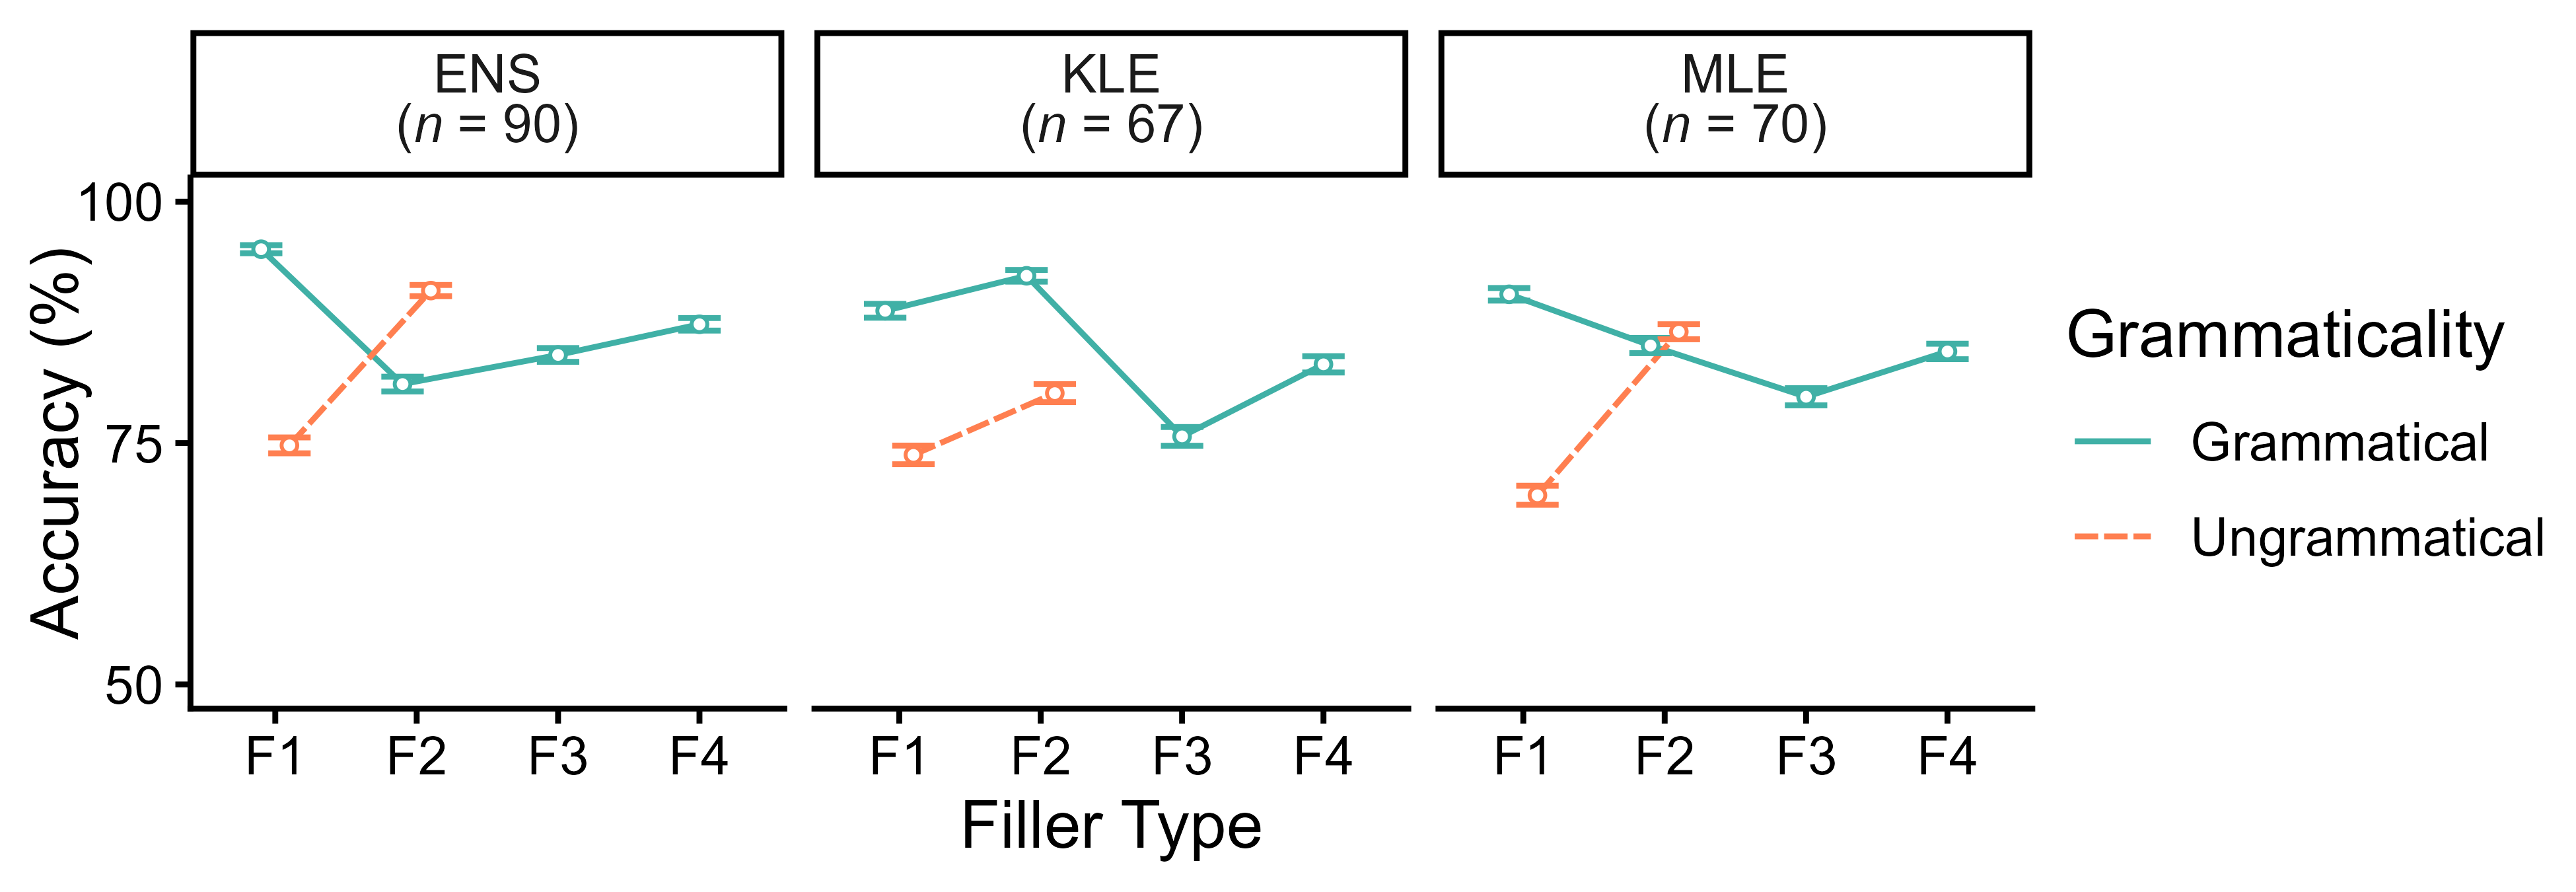
\includegraphics{../analysis/plots/orc_spr_accuracy_filler.png}
\textit{Note}. Error bars are 95\% $CI$s.
\vspace{-12pt}
\end{figure}

% SRC Figure
\begin{figure}
\caption{Percent accuracy for fillers in the SRC self-paced reading task} \label{fig:app-src-spr-accuracy-filler}
\raggedright\setstretch{1}
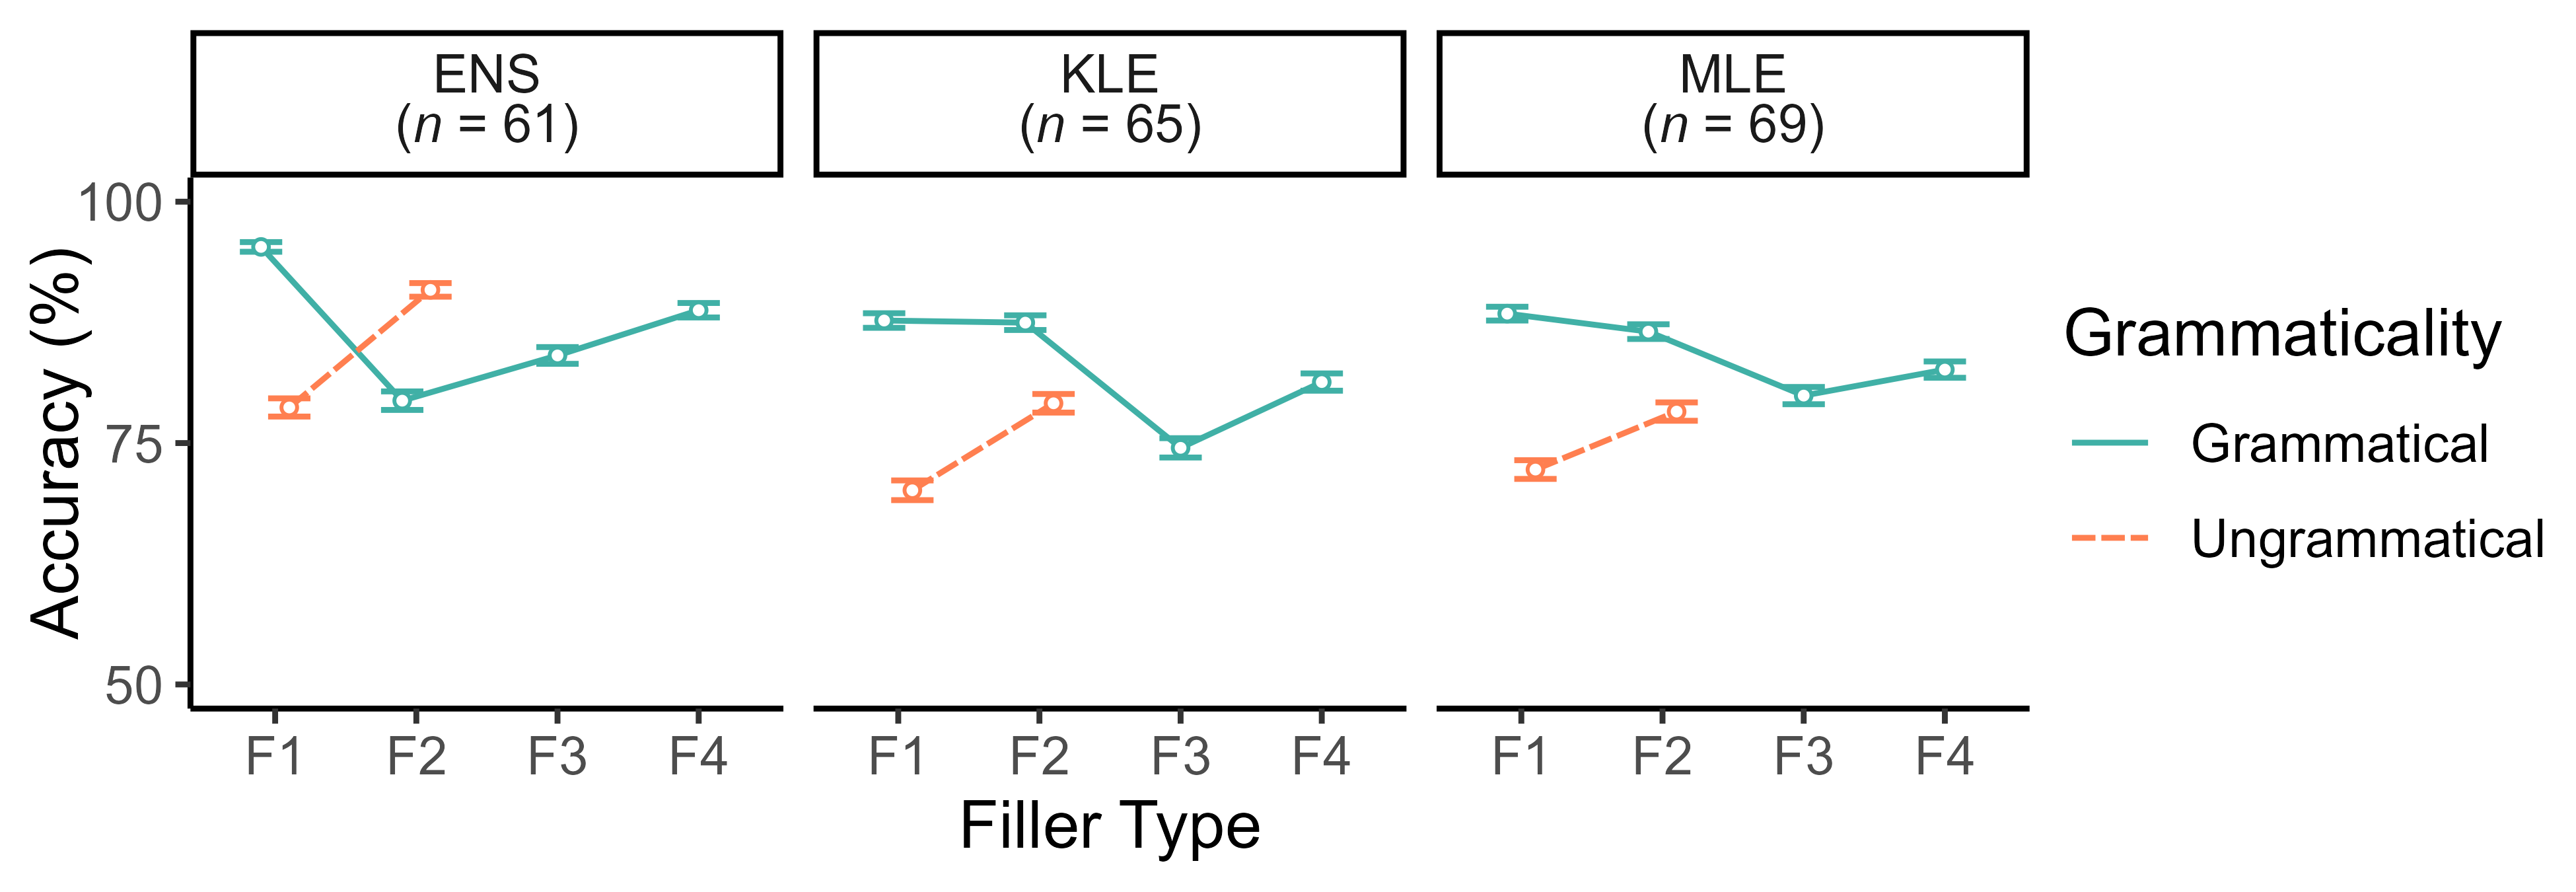
\includegraphics{../analysis/plots/src_spr_accuracy_filler.png}
\textit{Note}. Error bars are 95\% $CI$s.
\vspace{-12pt}
\end{figure}